% $Author: oscar $
% $Date: 2007-09-23 11:56:47 +0200 (Sun, 23 Sep 2007) $
% $Translation: martial $
% $Date: Wed Oct 10 17:22:05 CEST 2007 $
% $Revision: 12715 $ 
%=================================================================
% translated by Martial.Boniou@ifrance.com start: (Fri, 5 Oct 2007)
% relecture par Rene Mages : (Fri, 20 Dec 2007)
%=================================================================
\ifx\wholebook\relax\else
% --------------------------------------------
% Lulu:
	\documentclass[a4paper,10pt,twoside]{book}
	\usepackage[
		papersize={6in,9in},
		hmargin={.75in,.75in},
		vmargin={.75in,1in},
		ignoreheadfoot
	]{geometry}
	% $Author$ Martial
% $Date$ Wed Oct 10 13:34:55 CEST 2007
% $Revision$ source: SBE 12715 
% Last Changed Date: 2007-10-08 21:32:45 +0200 (Mon, 08 Oct 2007)
%=============================================================
% NB: documentclass must be set in main document.
% Allows book to be generated in multiple formats.
%=============================================================
%:Packages
\usepackage[french]{babel}
\usepackage[T1]{fontenc}  %%%%%% really important to get the code directly in the text!
\usepackage{lmodern}
%\usepackage[scaled=0.85]{bookmanx} % needs another scale factor if used with \renewcommand{\sfdefault}{cmbr}
\usepackage{palatino}
\usepackage[scaled=0.85]{helvet}
\usepackage{microtype}
\usepackage{graphicx}
\usepackage{theorem}
\usepackage[utf8]{inputenc}
% ON: pdfsync breaks the use of p{width} for tabular columns!
\ifdefined\usepdfsync\usepackage{pdfsync}\fi % Requires texlive 2007
%=============================================================
%:More packages
%Stef should check which ones are used!
%\usepackage{picinpar}
%\usepackage{layout}
%\usepackage{color}
%\usepackage{enum}
%\usepackage{a4wide}
% \usepackage{fancyhdr}
\usepackage{ifthen}
\usepackage{float}
\usepackage{longtable}
\usepackage{makeidx}
\usepackage[nottoc]{tocbibind}
\usepackage{multicol}
\usepackage{booktabs}	% book-style tables
\usepackage{topcapt}	% enables \topcaption
\usepackage{multirow}
\usepackage{tabularx}
%\usepackage[bottom]{footmisc}
\usepackage{xspace}
\usepackage{alltt}
\usepackage{amssymb,textcomp}
\usepackage[usenames,dvipsnames]{color}
%\usepackage{colortbl}
\usepackage[hang]{subfigure}\makeatletter\def\p@subfigure{\thefigure\,}\makeatother
\usepackage{rotating}
\usepackage{enumitem}	% apb: allows more control over tags in enumerations
\usepackage{verbatim}     % for comment environment
\usepackage{varioref}	% for page references that work
\labelformat{footnote}{\thechapter--#1} % to distinguish citations from jurabib
\usepackage{needspace}
\usepackage{isodateo} % enable \isodate
\usepackage[newparttoc]{titlesec}
\usepackage{titletoc}
\usepackage{eurosym}
\usepackage{wrapfig}

\usepackage[
	super,
	citefull=first,
	authorformat={allreversed,and},
	titleformat={commasep,italic}
]{jurabib} % citations as footnotes
\usepackage[
	colorlinks=true,
	linkcolor=black,
	urlcolor=black,
	citecolor=black
]{hyperref}   % should come last

%=============================================================
%:URL style
\makeatletter

\def\url@leostyle{%
  \@ifundefined{selectfont}{\def\UrlFont{\sf}}{\def\UrlFont{\sffamily}}}
% ajouter par Martial pour \traduit (met une dague dans les \doublebox
\def\thempfootnote{\fnsymbol{mpfootnote}}

\makeatother
% Now actually use the newly defined style.
\urlstyle{leo}
%=============================================================
%:Booleans
\newboolean{lulu}
\setboolean{lulu}{false}
\newcommand{\ifluluelse}[2]{\ifthenelse{\boolean{lulu}}{#1}{#2}}
%=============================================================
%:Names
\newcommand{\SUnit}{SUnit\xspace}
\newcommand{\sunit}{SUnit\xspace}
\newcommand{\xUnit}{$x$Unit\xspace}
\newcommand{\JUnit}{JUnit\xspace}
%\newcommand{\XP}{eXtreme Programming\xspace}
\newcommand{\st}{Smalltalk\xspace}
\newcommand{\Squeak}{Squeak\xspace}
\newcommand{\sq}{Squeak\xspace}
\newcommand{\sqmap}{SqueakMap\xspace}
\newcommand{\squeak}{Squeak\xspace}
%\newcommand{\sbe}{\url{scg.unibe.ch/SBE}\xspace}
%\newcommand{\sbe}{\url{squeakbyexample.org}\xspace}
\newcommand{\sbe}{\url{SqueakByExample.org}\xspace}
% squeak-fr: adresse de la version francaise
\newcommand{\spe}{\url{SqueakByExample.org}\xspace} % ?/FR
\newcommand{\sba}{\url{SquareBracketAssociates.org}\xspace}

% squeak-fr: ajout de la \squeakdev pour eviter les problemes de
% changements d'url rencontres dans la VO:
\newcommand{\squeakdev}{\url{www.squeaksource.com/ImageForDevelopers}\xspace} %ou
%\newcommand{\squeakdev}{\url{squeak.ofset.org/squeak-dev}\xspace}

%=============================================================
%:Editorial comment macros
\newcommand{\nnbb}[2]{
    \fbox{\bfseries\sffamily\scriptsize#1}
    {\sf\small$\blacktriangleright$\textit{#2}$\blacktriangleleft$}
   }
\newcommand{\ab}[1]{\nnbb{Andrew}{#1}}
\newcommand{\sd}[1]{\nnbb{St\'{e}f}{#1}}
\newcommand{\md}[1]{\nnbb{Marcus}{#1}}
\newcommand{\on}[1]{\nnbb{Oscar}{#1}}
\newcommand{\damien}[1]{\nnbb{Damien}{#1}}
\newcommand{\lr}[1]{\nnbb{Lukas}{#1}}
\newcommand{\orla}[1]{\nnbb{Orla}{#1}}
%\newcommand{\here}{\nnbb{CONTINUE}{HERE}}
\newcommand{\here}{\nnbb{CONTINUE}{ICI}}

%=============================================================
%:Abbreviation macros
\newcommand{\ie}{\emph{c-\`a-d.}\xspace}
\newcommand{\cad}{\emph{c-\`a-d.}\xspace}
%\newcommand{\eg}{\emph{e.g.},\xspace}
\newcommand{\eg}{\emph{par ex.},\xspace}
\newcommand{\parex}{\emph{par ex.},\xspace}
\newcommand{\etc}{etc\xspace}
%=============================================================
%:Cross reference macros

% [squeak-fr] martial: remarquez les articles devant les noms
\newcommand{\charef}[1]{le chapitre~\ref{cha:#1}\xspace}
% note de martial: utilise dans chapitre Syntax.tex: a redefinir
\newcommand{\charefs}[2]{les chapitres~\ref{cha:#1} et \ref{cha:#2}\xspace}
\newcommand{\secref}[1]{la section~\ref{sec:#1}\xspace}
\newcommand{\figref}[1]{la figure~\ref{fig:#1}\xspace}
\newcommand{\Figref}[1]{La figure~\ref{fig:#1}\xspace}
\newcommand{\appref}[1]{l'annexe~\ref{app:#1}\xspace}
\newcommand{\tabref}[1]{la table~\ref{tab:#1}\xspace}
% defini pour le chapitre Messages.tex
\newcommand{\Tabref}[1]{La table~\ref{tab:#1}\xspace}

% APB: I removed trailing \xspace commands from these macros because
% \xspace mostly doesn't work.  If you want a space after your
% references, type one!
% ON: xspace has always worked just fine for me!  Please leave them in.
%
\newcommand{\ruleref}[1]{\ref{rule:#1}\xspace}
%
\newcommand{\egref}[1]{exemple~\ref{eg:#1}\xspace}
\newcommand{\Egref}[1]{Exemple~\ref{eg:#1}\xspace}
%
\newcommand{\scrref}[1]{script~\ref{scr:#1}\xspace}
\newcommand{\Scrref}[1]{Script~\ref{scr:#1}\xspace}
% t = the
\newcommand{\tscrref}[1]{le script~\ref{scr:#1}\xspace}
\newcommand{\Tscrref}[1]{Le script~\ref{scr:#1}\xspace}
%
\newcommand{\mthref}[1]{m\'ethode~\ref{mth:#1}\xspace}
\newcommand{\mthsref}[1]{m\'ethodes~\ref{mth:#1}\xspace}
\newcommand{\Mthref}[1]{M\'ethode~\ref{mth:#1}\xspace}
\newcommand{\tmthref}[1]{la m\'ethode~\ref{mth:#1}\xspace}
\newcommand{\Tmthref}[1]{La m\'ethode~\ref{mth:#1}\xspace}
%
\newcommand{\clsref}[1]{classe~\ref{cls:#1}\xspace}
\newcommand{\tclsref}[1]{la classe~\ref{cls:#1}\xspace}
\newcommand{\Tclsref}[1]{La classe~\ref{cls:#1}\xspace}
%=============================================================
%:Menu item macro
% for menu items, so we can change our minds on how to print them! (apb)
\definecolor{lightgray}{gray}{0.89}
\newcommand{\menu}[1]{{%
	\setlength{\fboxsep}{0pt}%
	\colorbox{lightgray}{{{\upshape\sffamily\strut \,#1\,}}}}}
% \newcommand{\menu}[1]{{%
% 	\fontfamily{lmr}\selectfont
% 	\upshape\textlangle{\sffamily #1}\textrangle}}
% For submenu items:
\newcommand{\go}{\,$\triangleright$\,}
% \newcommand{\go}{\,$\blacktriangleright$\,}
% For keyboard shortcuts:
%\newcommand{\short}[1]{\mbox{$\langle${\sc CMD}$\rangle$-#1}\xspace}
\newcommand{\short}[1]{\mbox{{\sc cmd}\hspace{0.08em}--\hspace{0.09em}#1}\xspace}
% For buttons:
\newcommand{\button}[1]{{%
	\setlength{\fboxsep}{0pt}%
	\fbox{{\upshape\sffamily\strut \,#1\,}}}}
\newcommand{\toolsflap}{l'onglet \textit{Tools}\xspace}
%=============================================================
%:Reader cues (do this)
%
% Indicate something the reader should try out.
\newcommand{\dothisicon}{\raisebox{-.5ex}{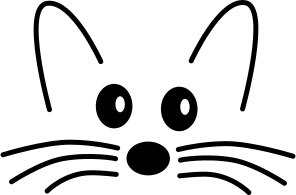
\includegraphics[width=1.4em]{squeak-logo}}}
\newcommand{\dothis}[1]{%
	\medskip
	\noindent\dothisicon
	\ifx#1\empty\else\quad\emph{#1}\fi
	\par\smallskip\nopagebreak}
% NB: To use this in an individual chapter, you must set:
%\graphicspath{{figures/} {../figures/}}
% at the head of the chapter.  Don't forget the final /
%=============================================================
%:Reader hints (hint)
%
% Indicates a non-obvious consequence 
\newcommand{\hint}[1]{\vspace{1ex}\noindent\fbox{\textsc{Astuce}} \emph{#1}}
%=================================================================
% graphics for Morphic handles
\newcommand{\grabHandle}{\raisebox{-0.2ex}{
\includegraphics[width=1em]{blackHandle}}}
\newcommand{\moveHandle}{\raisebox{-0.2ex}{
\includegraphics[width=1em]{moveHandle}}}
\newcommand{\debugHandle}{\raisebox{-0.2ex}{
\includegraphics[width=1em]{debugHandle}}}
% squeak-fr (added for Morphic handles)
\newcommand{\rotateHandle}{\raisebox{-0.2ex}{
\includegraphics[width=1em]{rotateHandle}}}
\newcommand{\viewerHandle}{\raisebox{-0.2ex}{
\includegraphics[width=1em]{viewerHandle}}}
% squeak-fr (add cloverHandle to use \clover in QuickTour.tex as alias
% todo 

%=============================================================
%:Highlighting Important stuff (doublebox)
%
% From Seaside book ...
\newsavebox{\SavedText}
\newlength{\InnerBoxRule}\setlength{\InnerBoxRule}{.75\fboxrule}
\newlength{\OuterBoxRule}\setlength{\OuterBoxRule}{1.5\fboxrule}
\newlength{\BoxSeparation}\setlength{\BoxSeparation}{1.5\fboxrule}
\addtolength{\BoxSeparation}{.5pt}
\newlength{\SaveBoxSep}\setlength{\SaveBoxSep}{2\fboxsep}
%
\newenvironment{doublebox}{\begin{lrbox}{\SavedText}
    \begin{minipage}{.75\textwidth}}
    {\end{minipage}\end{lrbox}\begin{center}
    \setlength{\fboxsep}{\BoxSeparation}\setlength{\fboxrule}{\OuterBoxRule}
    \fbox{\setlength{\fboxsep}{\SaveBoxSep}\setlength{\fboxrule}{\InnerBoxRule}%
      \fbox{\usebox{\SavedText}}}
  \end{center}}
% Use this:
\newcommand{\important}[1]{\begin{doublebox}#1\end{doublebox}}
%=============================================================
%:Section depth
\setcounter{secnumdepth}{2}
%% for this to happen start the file with
%\ifx\wholebook\relax\else
%% $Author$ Martial
% $Date$ Wed Oct 10 13:34:55 CEST 2007
% $Revision$ source: SBE 12715 
% Last Changed Date: 2007-10-08 21:32:45 +0200 (Mon, 08 Oct 2007)
%=============================================================
% NB: documentclass must be set in main document.
% Allows book to be generated in multiple formats.
%=============================================================
%:Packages
\usepackage[french]{babel}
\usepackage[T1]{fontenc}  %%%%%% really important to get the code directly in the text!
\usepackage{lmodern}
%\usepackage[scaled=0.85]{bookmanx} % needs another scale factor if used with \renewcommand{\sfdefault}{cmbr}
\usepackage{palatino}
\usepackage[scaled=0.85]{helvet}
\usepackage{microtype}
\usepackage{graphicx}
\usepackage{theorem}
\usepackage[utf8]{inputenc}
% ON: pdfsync breaks the use of p{width} for tabular columns!
\ifdefined\usepdfsync\usepackage{pdfsync}\fi % Requires texlive 2007
%=============================================================
%:More packages
%Stef should check which ones are used!
%\usepackage{picinpar}
%\usepackage{layout}
%\usepackage{color}
%\usepackage{enum}
%\usepackage{a4wide}
% \usepackage{fancyhdr}
\usepackage{ifthen}
\usepackage{float}
\usepackage{longtable}
\usepackage{makeidx}
\usepackage[nottoc]{tocbibind}
\usepackage{multicol}
\usepackage{booktabs}	% book-style tables
\usepackage{topcapt}	% enables \topcaption
\usepackage{multirow}
\usepackage{tabularx}
%\usepackage[bottom]{footmisc}
\usepackage{xspace}
\usepackage{alltt}
\usepackage{amssymb,textcomp}
\usepackage[usenames,dvipsnames]{color}
%\usepackage{colortbl}
\usepackage[hang]{subfigure}\makeatletter\def\p@subfigure{\thefigure\,}\makeatother
\usepackage{rotating}
\usepackage{enumitem}	% apb: allows more control over tags in enumerations
\usepackage{verbatim}     % for comment environment
\usepackage{varioref}	% for page references that work
\labelformat{footnote}{\thechapter--#1} % to distinguish citations from jurabib
\usepackage{needspace}
\usepackage{isodateo} % enable \isodate
\usepackage[newparttoc]{titlesec}
\usepackage{titletoc}
\usepackage{eurosym}
\usepackage{wrapfig}

\usepackage[
	super,
	citefull=first,
	authorformat={allreversed,and},
	titleformat={commasep,italic}
]{jurabib} % citations as footnotes
\usepackage[
	colorlinks=true,
	linkcolor=black,
	urlcolor=black,
	citecolor=black
]{hyperref}   % should come last

%=============================================================
%:URL style
\makeatletter

\def\url@leostyle{%
  \@ifundefined{selectfont}{\def\UrlFont{\sf}}{\def\UrlFont{\sffamily}}}
% ajouter par Martial pour \traduit (met une dague dans les \doublebox
\def\thempfootnote{\fnsymbol{mpfootnote}}

\makeatother
% Now actually use the newly defined style.
\urlstyle{leo}
%=============================================================
%:Booleans
\newboolean{lulu}
\setboolean{lulu}{false}
\newcommand{\ifluluelse}[2]{\ifthenelse{\boolean{lulu}}{#1}{#2}}
%=============================================================
%:Names
\newcommand{\SUnit}{SUnit\xspace}
\newcommand{\sunit}{SUnit\xspace}
\newcommand{\xUnit}{$x$Unit\xspace}
\newcommand{\JUnit}{JUnit\xspace}
%\newcommand{\XP}{eXtreme Programming\xspace}
\newcommand{\st}{Smalltalk\xspace}
\newcommand{\Squeak}{Squeak\xspace}
\newcommand{\sq}{Squeak\xspace}
\newcommand{\sqmap}{SqueakMap\xspace}
\newcommand{\squeak}{Squeak\xspace}
%\newcommand{\sbe}{\url{scg.unibe.ch/SBE}\xspace}
%\newcommand{\sbe}{\url{squeakbyexample.org}\xspace}
\newcommand{\sbe}{\url{SqueakByExample.org}\xspace}
% squeak-fr: adresse de la version francaise
\newcommand{\spe}{\url{SqueakByExample.org}\xspace} % ?/FR
\newcommand{\sba}{\url{SquareBracketAssociates.org}\xspace}

% squeak-fr: ajout de la \squeakdev pour eviter les problemes de
% changements d'url rencontres dans la VO:
\newcommand{\squeakdev}{\url{www.squeaksource.com/ImageForDevelopers}\xspace} %ou
%\newcommand{\squeakdev}{\url{squeak.ofset.org/squeak-dev}\xspace}

%=============================================================
%:Editorial comment macros
\newcommand{\nnbb}[2]{
    \fbox{\bfseries\sffamily\scriptsize#1}
    {\sf\small$\blacktriangleright$\textit{#2}$\blacktriangleleft$}
   }
\newcommand{\ab}[1]{\nnbb{Andrew}{#1}}
\newcommand{\sd}[1]{\nnbb{St\'{e}f}{#1}}
\newcommand{\md}[1]{\nnbb{Marcus}{#1}}
\newcommand{\on}[1]{\nnbb{Oscar}{#1}}
\newcommand{\damien}[1]{\nnbb{Damien}{#1}}
\newcommand{\lr}[1]{\nnbb{Lukas}{#1}}
\newcommand{\orla}[1]{\nnbb{Orla}{#1}}
%\newcommand{\here}{\nnbb{CONTINUE}{HERE}}
\newcommand{\here}{\nnbb{CONTINUE}{ICI}}

%=============================================================
%:Abbreviation macros
\newcommand{\ie}{\emph{c-\`a-d.}\xspace}
\newcommand{\cad}{\emph{c-\`a-d.}\xspace}
%\newcommand{\eg}{\emph{e.g.},\xspace}
\newcommand{\eg}{\emph{par ex.},\xspace}
\newcommand{\parex}{\emph{par ex.},\xspace}
\newcommand{\etc}{etc\xspace}
%=============================================================
%:Cross reference macros

% [squeak-fr] martial: remarquez les articles devant les noms
\newcommand{\charef}[1]{le chapitre~\ref{cha:#1}\xspace}
% note de martial: utilise dans chapitre Syntax.tex: a redefinir
\newcommand{\charefs}[2]{les chapitres~\ref{cha:#1} et \ref{cha:#2}\xspace}
\newcommand{\secref}[1]{la section~\ref{sec:#1}\xspace}
\newcommand{\figref}[1]{la figure~\ref{fig:#1}\xspace}
\newcommand{\Figref}[1]{La figure~\ref{fig:#1}\xspace}
\newcommand{\appref}[1]{l'annexe~\ref{app:#1}\xspace}
\newcommand{\tabref}[1]{la table~\ref{tab:#1}\xspace}
% defini pour le chapitre Messages.tex
\newcommand{\Tabref}[1]{La table~\ref{tab:#1}\xspace}

% APB: I removed trailing \xspace commands from these macros because
% \xspace mostly doesn't work.  If you want a space after your
% references, type one!
% ON: xspace has always worked just fine for me!  Please leave them in.
%
\newcommand{\ruleref}[1]{\ref{rule:#1}\xspace}
%
\newcommand{\egref}[1]{exemple~\ref{eg:#1}\xspace}
\newcommand{\Egref}[1]{Exemple~\ref{eg:#1}\xspace}
%
\newcommand{\scrref}[1]{script~\ref{scr:#1}\xspace}
\newcommand{\Scrref}[1]{Script~\ref{scr:#1}\xspace}
% t = the
\newcommand{\tscrref}[1]{le script~\ref{scr:#1}\xspace}
\newcommand{\Tscrref}[1]{Le script~\ref{scr:#1}\xspace}
%
\newcommand{\mthref}[1]{m\'ethode~\ref{mth:#1}\xspace}
\newcommand{\mthsref}[1]{m\'ethodes~\ref{mth:#1}\xspace}
\newcommand{\Mthref}[1]{M\'ethode~\ref{mth:#1}\xspace}
\newcommand{\tmthref}[1]{la m\'ethode~\ref{mth:#1}\xspace}
\newcommand{\Tmthref}[1]{La m\'ethode~\ref{mth:#1}\xspace}
%
\newcommand{\clsref}[1]{classe~\ref{cls:#1}\xspace}
\newcommand{\tclsref}[1]{la classe~\ref{cls:#1}\xspace}
\newcommand{\Tclsref}[1]{La classe~\ref{cls:#1}\xspace}
%=============================================================
%:Menu item macro
% for menu items, so we can change our minds on how to print them! (apb)
\definecolor{lightgray}{gray}{0.89}
\newcommand{\menu}[1]{{%
	\setlength{\fboxsep}{0pt}%
	\colorbox{lightgray}{{{\upshape\sffamily\strut \,#1\,}}}}}
% \newcommand{\menu}[1]{{%
% 	\fontfamily{lmr}\selectfont
% 	\upshape\textlangle{\sffamily #1}\textrangle}}
% For submenu items:
\newcommand{\go}{\,$\triangleright$\,}
% \newcommand{\go}{\,$\blacktriangleright$\,}
% For keyboard shortcuts:
%\newcommand{\short}[1]{\mbox{$\langle${\sc CMD}$\rangle$-#1}\xspace}
\newcommand{\short}[1]{\mbox{{\sc cmd}\hspace{0.08em}--\hspace{0.09em}#1}\xspace}
% For buttons:
\newcommand{\button}[1]{{%
	\setlength{\fboxsep}{0pt}%
	\fbox{{\upshape\sffamily\strut \,#1\,}}}}
\newcommand{\toolsflap}{l'onglet \textit{Tools}\xspace}
%=============================================================
%:Reader cues (do this)
%
% Indicate something the reader should try out.
\newcommand{\dothisicon}{\raisebox{-.5ex}{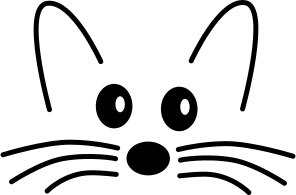
\includegraphics[width=1.4em]{squeak-logo}}}
\newcommand{\dothis}[1]{%
	\medskip
	\noindent\dothisicon
	\ifx#1\empty\else\quad\emph{#1}\fi
	\par\smallskip\nopagebreak}
% NB: To use this in an individual chapter, you must set:
%\graphicspath{{figures/} {../figures/}}
% at the head of the chapter.  Don't forget the final /
%=============================================================
%:Reader hints (hint)
%
% Indicates a non-obvious consequence 
\newcommand{\hint}[1]{\vspace{1ex}\noindent\fbox{\textsc{Astuce}} \emph{#1}}
%=================================================================
% graphics for Morphic handles
\newcommand{\grabHandle}{\raisebox{-0.2ex}{
\includegraphics[width=1em]{blackHandle}}}
\newcommand{\moveHandle}{\raisebox{-0.2ex}{
\includegraphics[width=1em]{moveHandle}}}
\newcommand{\debugHandle}{\raisebox{-0.2ex}{
\includegraphics[width=1em]{debugHandle}}}
% squeak-fr (added for Morphic handles)
\newcommand{\rotateHandle}{\raisebox{-0.2ex}{
\includegraphics[width=1em]{rotateHandle}}}
\newcommand{\viewerHandle}{\raisebox{-0.2ex}{
\includegraphics[width=1em]{viewerHandle}}}
% squeak-fr (add cloverHandle to use \clover in QuickTour.tex as alias
% todo 

%=============================================================
%:Highlighting Important stuff (doublebox)
%
% From Seaside book ...
\newsavebox{\SavedText}
\newlength{\InnerBoxRule}\setlength{\InnerBoxRule}{.75\fboxrule}
\newlength{\OuterBoxRule}\setlength{\OuterBoxRule}{1.5\fboxrule}
\newlength{\BoxSeparation}\setlength{\BoxSeparation}{1.5\fboxrule}
\addtolength{\BoxSeparation}{.5pt}
\newlength{\SaveBoxSep}\setlength{\SaveBoxSep}{2\fboxsep}
%
\newenvironment{doublebox}{\begin{lrbox}{\SavedText}
    \begin{minipage}{.75\textwidth}}
    {\end{minipage}\end{lrbox}\begin{center}
    \setlength{\fboxsep}{\BoxSeparation}\setlength{\fboxrule}{\OuterBoxRule}
    \fbox{\setlength{\fboxsep}{\SaveBoxSep}\setlength{\fboxrule}{\InnerBoxRule}%
      \fbox{\usebox{\SavedText}}}
  \end{center}}
% Use this:
\newcommand{\important}[1]{\begin{doublebox}#1\end{doublebox}}
%=============================================================
%:Section depth
\setcounter{secnumdepth}{2}
%% for this to happen start the file with
%\ifx\wholebook\relax\else
%% $Author$ Martial
% $Date$ Wed Oct 10 13:34:55 CEST 2007
% $Revision$ source: SBE 12715 
% Last Changed Date: 2007-10-08 21:32:45 +0200 (Mon, 08 Oct 2007)
%=============================================================
% NB: documentclass must be set in main document.
% Allows book to be generated in multiple formats.
%=============================================================
%:Packages
\usepackage[french]{babel}
\usepackage[T1]{fontenc}  %%%%%% really important to get the code directly in the text!
\usepackage{lmodern}
%\usepackage[scaled=0.85]{bookmanx} % needs another scale factor if used with \renewcommand{\sfdefault}{cmbr}
\usepackage{palatino}
\usepackage[scaled=0.85]{helvet}
\usepackage{microtype}
\usepackage{graphicx}
\usepackage{theorem}
\usepackage[utf8]{inputenc}
% ON: pdfsync breaks the use of p{width} for tabular columns!
\ifdefined\usepdfsync\usepackage{pdfsync}\fi % Requires texlive 2007
%=============================================================
%:More packages
%Stef should check which ones are used!
%\usepackage{picinpar}
%\usepackage{layout}
%\usepackage{color}
%\usepackage{enum}
%\usepackage{a4wide}
% \usepackage{fancyhdr}
\usepackage{ifthen}
\usepackage{float}
\usepackage{longtable}
\usepackage{makeidx}
\usepackage[nottoc]{tocbibind}
\usepackage{multicol}
\usepackage{booktabs}	% book-style tables
\usepackage{topcapt}	% enables \topcaption
\usepackage{multirow}
\usepackage{tabularx}
%\usepackage[bottom]{footmisc}
\usepackage{xspace}
\usepackage{alltt}
\usepackage{amssymb,textcomp}
\usepackage[usenames,dvipsnames]{color}
%\usepackage{colortbl}
\usepackage[hang]{subfigure}\makeatletter\def\p@subfigure{\thefigure\,}\makeatother
\usepackage{rotating}
\usepackage{enumitem}	% apb: allows more control over tags in enumerations
\usepackage{verbatim}     % for comment environment
\usepackage{varioref}	% for page references that work
\labelformat{footnote}{\thechapter--#1} % to distinguish citations from jurabib
\usepackage{needspace}
\usepackage{isodateo} % enable \isodate
\usepackage[newparttoc]{titlesec}
\usepackage{titletoc}
\usepackage{eurosym}
\usepackage{wrapfig}

\usepackage[
	super,
	citefull=first,
	authorformat={allreversed,and},
	titleformat={commasep,italic}
]{jurabib} % citations as footnotes
\usepackage[
	colorlinks=true,
	linkcolor=black,
	urlcolor=black,
	citecolor=black
]{hyperref}   % should come last

%=============================================================
%:URL style
\makeatletter

\def\url@leostyle{%
  \@ifundefined{selectfont}{\def\UrlFont{\sf}}{\def\UrlFont{\sffamily}}}
% ajouter par Martial pour \traduit (met une dague dans les \doublebox
\def\thempfootnote{\fnsymbol{mpfootnote}}

\makeatother
% Now actually use the newly defined style.
\urlstyle{leo}
%=============================================================
%:Booleans
\newboolean{lulu}
\setboolean{lulu}{false}
\newcommand{\ifluluelse}[2]{\ifthenelse{\boolean{lulu}}{#1}{#2}}
%=============================================================
%:Names
\newcommand{\SUnit}{SUnit\xspace}
\newcommand{\sunit}{SUnit\xspace}
\newcommand{\xUnit}{$x$Unit\xspace}
\newcommand{\JUnit}{JUnit\xspace}
%\newcommand{\XP}{eXtreme Programming\xspace}
\newcommand{\st}{Smalltalk\xspace}
\newcommand{\Squeak}{Squeak\xspace}
\newcommand{\sq}{Squeak\xspace}
\newcommand{\sqmap}{SqueakMap\xspace}
\newcommand{\squeak}{Squeak\xspace}
%\newcommand{\sbe}{\url{scg.unibe.ch/SBE}\xspace}
%\newcommand{\sbe}{\url{squeakbyexample.org}\xspace}
\newcommand{\sbe}{\url{SqueakByExample.org}\xspace}
% squeak-fr: adresse de la version francaise
\newcommand{\spe}{\url{SqueakByExample.org}\xspace} % ?/FR
\newcommand{\sba}{\url{SquareBracketAssociates.org}\xspace}

% squeak-fr: ajout de la \squeakdev pour eviter les problemes de
% changements d'url rencontres dans la VO:
\newcommand{\squeakdev}{\url{www.squeaksource.com/ImageForDevelopers}\xspace} %ou
%\newcommand{\squeakdev}{\url{squeak.ofset.org/squeak-dev}\xspace}

%=============================================================
%:Editorial comment macros
\newcommand{\nnbb}[2]{
    \fbox{\bfseries\sffamily\scriptsize#1}
    {\sf\small$\blacktriangleright$\textit{#2}$\blacktriangleleft$}
   }
\newcommand{\ab}[1]{\nnbb{Andrew}{#1}}
\newcommand{\sd}[1]{\nnbb{St\'{e}f}{#1}}
\newcommand{\md}[1]{\nnbb{Marcus}{#1}}
\newcommand{\on}[1]{\nnbb{Oscar}{#1}}
\newcommand{\damien}[1]{\nnbb{Damien}{#1}}
\newcommand{\lr}[1]{\nnbb{Lukas}{#1}}
\newcommand{\orla}[1]{\nnbb{Orla}{#1}}
%\newcommand{\here}{\nnbb{CONTINUE}{HERE}}
\newcommand{\here}{\nnbb{CONTINUE}{ICI}}

%=============================================================
%:Abbreviation macros
\newcommand{\ie}{\emph{c-\`a-d.}\xspace}
\newcommand{\cad}{\emph{c-\`a-d.}\xspace}
%\newcommand{\eg}{\emph{e.g.},\xspace}
\newcommand{\eg}{\emph{par ex.},\xspace}
\newcommand{\parex}{\emph{par ex.},\xspace}
\newcommand{\etc}{etc\xspace}
%=============================================================
%:Cross reference macros

% [squeak-fr] martial: remarquez les articles devant les noms
\newcommand{\charef}[1]{le chapitre~\ref{cha:#1}\xspace}
% note de martial: utilise dans chapitre Syntax.tex: a redefinir
\newcommand{\charefs}[2]{les chapitres~\ref{cha:#1} et \ref{cha:#2}\xspace}
\newcommand{\secref}[1]{la section~\ref{sec:#1}\xspace}
\newcommand{\figref}[1]{la figure~\ref{fig:#1}\xspace}
\newcommand{\Figref}[1]{La figure~\ref{fig:#1}\xspace}
\newcommand{\appref}[1]{l'annexe~\ref{app:#1}\xspace}
\newcommand{\tabref}[1]{la table~\ref{tab:#1}\xspace}
% defini pour le chapitre Messages.tex
\newcommand{\Tabref}[1]{La table~\ref{tab:#1}\xspace}

% APB: I removed trailing \xspace commands from these macros because
% \xspace mostly doesn't work.  If you want a space after your
% references, type one!
% ON: xspace has always worked just fine for me!  Please leave them in.
%
\newcommand{\ruleref}[1]{\ref{rule:#1}\xspace}
%
\newcommand{\egref}[1]{exemple~\ref{eg:#1}\xspace}
\newcommand{\Egref}[1]{Exemple~\ref{eg:#1}\xspace}
%
\newcommand{\scrref}[1]{script~\ref{scr:#1}\xspace}
\newcommand{\Scrref}[1]{Script~\ref{scr:#1}\xspace}
% t = the
\newcommand{\tscrref}[1]{le script~\ref{scr:#1}\xspace}
\newcommand{\Tscrref}[1]{Le script~\ref{scr:#1}\xspace}
%
\newcommand{\mthref}[1]{m\'ethode~\ref{mth:#1}\xspace}
\newcommand{\mthsref}[1]{m\'ethodes~\ref{mth:#1}\xspace}
\newcommand{\Mthref}[1]{M\'ethode~\ref{mth:#1}\xspace}
\newcommand{\tmthref}[1]{la m\'ethode~\ref{mth:#1}\xspace}
\newcommand{\Tmthref}[1]{La m\'ethode~\ref{mth:#1}\xspace}
%
\newcommand{\clsref}[1]{classe~\ref{cls:#1}\xspace}
\newcommand{\tclsref}[1]{la classe~\ref{cls:#1}\xspace}
\newcommand{\Tclsref}[1]{La classe~\ref{cls:#1}\xspace}
%=============================================================
%:Menu item macro
% for menu items, so we can change our minds on how to print them! (apb)
\definecolor{lightgray}{gray}{0.89}
\newcommand{\menu}[1]{{%
	\setlength{\fboxsep}{0pt}%
	\colorbox{lightgray}{{{\upshape\sffamily\strut \,#1\,}}}}}
% \newcommand{\menu}[1]{{%
% 	\fontfamily{lmr}\selectfont
% 	\upshape\textlangle{\sffamily #1}\textrangle}}
% For submenu items:
\newcommand{\go}{\,$\triangleright$\,}
% \newcommand{\go}{\,$\blacktriangleright$\,}
% For keyboard shortcuts:
%\newcommand{\short}[1]{\mbox{$\langle${\sc CMD}$\rangle$-#1}\xspace}
\newcommand{\short}[1]{\mbox{{\sc cmd}\hspace{0.08em}--\hspace{0.09em}#1}\xspace}
% For buttons:
\newcommand{\button}[1]{{%
	\setlength{\fboxsep}{0pt}%
	\fbox{{\upshape\sffamily\strut \,#1\,}}}}
\newcommand{\toolsflap}{l'onglet \textit{Tools}\xspace}
%=============================================================
%:Reader cues (do this)
%
% Indicate something the reader should try out.
\newcommand{\dothisicon}{\raisebox{-.5ex}{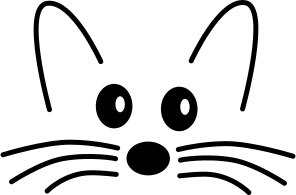
\includegraphics[width=1.4em]{squeak-logo}}}
\newcommand{\dothis}[1]{%
	\medskip
	\noindent\dothisicon
	\ifx#1\empty\else\quad\emph{#1}\fi
	\par\smallskip\nopagebreak}
% NB: To use this in an individual chapter, you must set:
%\graphicspath{{figures/} {../figures/}}
% at the head of the chapter.  Don't forget the final /
%=============================================================
%:Reader hints (hint)
%
% Indicates a non-obvious consequence 
\newcommand{\hint}[1]{\vspace{1ex}\noindent\fbox{\textsc{Astuce}} \emph{#1}}
%=================================================================
% graphics for Morphic handles
\newcommand{\grabHandle}{\raisebox{-0.2ex}{
\includegraphics[width=1em]{blackHandle}}}
\newcommand{\moveHandle}{\raisebox{-0.2ex}{
\includegraphics[width=1em]{moveHandle}}}
\newcommand{\debugHandle}{\raisebox{-0.2ex}{
\includegraphics[width=1em]{debugHandle}}}
% squeak-fr (added for Morphic handles)
\newcommand{\rotateHandle}{\raisebox{-0.2ex}{
\includegraphics[width=1em]{rotateHandle}}}
\newcommand{\viewerHandle}{\raisebox{-0.2ex}{
\includegraphics[width=1em]{viewerHandle}}}
% squeak-fr (add cloverHandle to use \clover in QuickTour.tex as alias
% todo 

%=============================================================
%:Highlighting Important stuff (doublebox)
%
% From Seaside book ...
\newsavebox{\SavedText}
\newlength{\InnerBoxRule}\setlength{\InnerBoxRule}{.75\fboxrule}
\newlength{\OuterBoxRule}\setlength{\OuterBoxRule}{1.5\fboxrule}
\newlength{\BoxSeparation}\setlength{\BoxSeparation}{1.5\fboxrule}
\addtolength{\BoxSeparation}{.5pt}
\newlength{\SaveBoxSep}\setlength{\SaveBoxSep}{2\fboxsep}
%
\newenvironment{doublebox}{\begin{lrbox}{\SavedText}
    \begin{minipage}{.75\textwidth}}
    {\end{minipage}\end{lrbox}\begin{center}
    \setlength{\fboxsep}{\BoxSeparation}\setlength{\fboxrule}{\OuterBoxRule}
    \fbox{\setlength{\fboxsep}{\SaveBoxSep}\setlength{\fboxrule}{\InnerBoxRule}%
      \fbox{\usebox{\SavedText}}}
  \end{center}}
% Use this:
\newcommand{\important}[1]{\begin{doublebox}#1\end{doublebox}}
%=============================================================
%:Section depth
\setcounter{secnumdepth}{2}
%% for this to happen start the file with
%\ifx\wholebook\relax\else
%\input{../common.tex}
%\begin{document}
%\fi
% and terminate by
% \ifx\wholebook\relax\else\end{document}\fi

\DeclareGraphicsExtensions{.pdf, .jpg, .png}
%=============================================================
%:PDF setup
\hypersetup{
%   a4paper,
%   pdfstartview=FitV,
%   colorlinks,
%   linkcolor=darkblue,
%   citecolor=darkblue,
%   pdftitle={Squeak by Example},
pdftitle={Squeak par l'exemple},
   pdfauthor={Andrew Black, St\'ephane Ducasse,	Oscar Nierstrasz,
Damien Pollet},
   pdfkeywords={Smalltalk, Squeak, Programmation Orient\'ee Objet},
pdfsubject={Informatique, Computer Science}
}
%=============================================================
%:Page layout and appearance
%
% \renewcommand{\headrulewidth}{0pt}
\renewcommand{\chaptermark}[1]{\markboth{#1}{}}
\renewcommand{\sectionmark}[1]{\markright{\thesection\ #1}}
\renewpagestyle{plain}[\small\itshape]{%
	\setheadrule{0pt}%
	\sethead[\thepage][][]{}{}{\thepage}%
	\setfoot[][][]{}{}{}}
\renewpagestyle{headings}[\small\itshape]{%
	\setheadrule{0pt}%
	\setmarks{chapter}{section}%
	\sethead[\thepage][][\chaptertitle]{\sectiontitle}{}{\thepage}%
	\setfoot[][][]{}{}{}}
%=============================================================
%:Title section setup and TOC numbering depth
\setcounter{secnumdepth}{1}
\setcounter{tocdepth}{1}
\titleformat{\part}[display]{\centering}{\huge\partname\ \thepart}{1em}{\Huge\textbf}[]
\titleformat{\chapter}[display]{}{\huge\chaptertitlename\ \thechapter}{1em}{\Huge\raggedright\textbf}[]
\titlecontents{part}[3pc]{%
		\pagebreak[2]\addvspace{1em plus.4em minus.2em}%
		\leavevmode\large\bfseries}
	{\contentslabel{3pc}}{\hspace*{-3pc}}
	{}[\nopagebreak]
\titlecontents{chapter}[3pc]{%
		\pagebreak[0]\addvspace{1em plus.2em minus.2em}%
		\leavevmode\bfseries}
	{\contentslabel{3pc}}{}
	{\hfill\contentspage}[\nopagebreak]
\dottedcontents{section}[3pc]{}{3pc}{1pc}
\dottedcontents{subsection}[3pc]{}{0pc}{1pc}
% \dottedcontents{subsection}[4.5em]{}{0pt}{1pc}
% Make \cleardoublepage insert really blank pages http://www.tex.ac.uk/cgi-bin/texfaq2html?label=reallyblank
\let\origdoublepage\cleardoublepage
\newcommand{\clearemptydoublepage}{%
  \clearpage
  {\pagestyle{empty}\origdoublepage}}
\let\cleardoublepage\clearemptydoublepage % see http://www.tex.ac.uk/cgi-bin/texfaq2html?label=patch
%=============================================================
%:FAQ macros (for FAQ chapter)
\newtheorem{faq}{FAQ}
\newcommand{\answer}{\paragraph{R\'eponse}\ }
%=============================================================
%:Listings package configuration
\usepackage{listings}
\newcommand{\caret}{\makebox{\raisebox{0.4ex}{\footnotesize{$\wedge$}}}}
\lstdefinelanguage{Smalltalk}{
%  morekeywords={self,super,true,false,nil,thisContext}, % This is overkill
  morestring=[d]',
  morecomment=[s]{"}{"},
  alsoletter={\#:},
  escapechar={!},
  escapebegin=\itshape, % comment-like by default (Martial 11/2007)
  literate=
    {BANG}{!}1
    {UNDERSCORE}{\_}1
    {\\st}{Smalltalk}9 % convenience -- in case \st occurs in code
    % {'}{{\textquotesingle}}1 % replaced by upquote=true in \lstset
    {_}{{$\leftarrow$}}1
    {>>>}{{\sep}}1
    {^}{{$\uparrow$}}1
    {~}{{$\sim$}}1
    {-}{{\sf -\hspace{-0.13em}-}}1  % the goal is to make - the same width as +
    {+}{\raisebox{0.08ex}{+}}1		% and to raise + off the baseline to match -
    {-->}{{\quad$\longrightarrow$\quad}}3
	, % Don't forget the comma at the end!
  tabsize=4
}[keywords,comments,strings]
% ajout pour les échappements dans les codes
% indispensable pour mettre le code en emphase (cf. Model.tex) 
\newcommand{\codeify}[1]{\NoAutoSpaceBeforeFDP#1\AutoSpaceBeforeFDP}
\newcommand{\normcomment}[1]{\emph{#1}} %cf. Streams
\newcommand{\normcode}[1]{\emph{\codeify{#1}}} %cf. Streams
\newcommand{\emcode}[1]{\textbf{\normcode{#1}}} % Martial 11/2007
\lstset{language=Smalltalk,
	basicstyle=\sffamily,
	keywordstyle=\color{black}\bfseries,
	% stringstyle=\ttfamily, % Ugly! do we really want this? -- on
	%commentstyle=\itshape,
	mathescape=true,
	showstringspaces=false,
	keepspaces=true,
	breaklines=true,
	breakautoindent=true,
	lineskip={-1pt}, % Ugly hack
	upquote=true, % straight quote; requires textcomp package
	columns=fullflexible} % no fixed width fonts
% In-line code (literal)
% Normally use this for all in-line code:
\newcommand{\ct}{\lstinline[mathescape=false,basicstyle={\sffamily\upshape}]}
% apb 2007.8.28 added the \upshape declaration to avoid getting italicized code in \dothis{ } sections.
% In-line code (latex enabled)
% Use this only in special situations where \ct does not work
% (within section headings ...):

% [squeak-fr] Modification de \lct suivant les indications de Martial Boniou
\newcommand{\lct}[1]{\textsf{\textup{\NoAutoSpaceBeforeFDP #1
\AutoSpaceBeforeFDP}}} %\xspace

% Use these for system categories and protocols:
\newcommand{\scat}[1]{\emph{\textsf{#1}}\xspace}
\newcommand{\pkg}[1]{\emph{\textsf{#1}}\xspace}
\newcommand{\prot}[1]{\emph{\textsf{#1}}\xspace}
% Code environments
% NB: the arg is for tests
% Only code and example environments may be tests
\lstnewenvironment{code}[1]{%
	\lstset{%
		frame=lines,
		mathescape=false
	}
}{}
\def\ignoredollar#1{}
%=============================================================
%:Code environments (method, script ...)
% NB: the third arg is for tests
% Only code and example environments may be tests
\lstnewenvironment{example}[3][defaultlabel]{%
	\renewcommand{\lstlistingname}{Exemple}%
	\lstset{
		frame=lines,
		mathescape=false,
		caption={\emph{#2}},
		label={eg:#1}
	}
}{}
\lstnewenvironment{script}[2][defaultlabel]{%
\renewcommand{\lstlistingname}{Script}%
	\lstset{
		frame=lines,
		mathescape=false,
		name={Script},
		caption={\emph{#2}},
		label={scr:#1}
	}
}{}
\lstnewenvironment{method}[2][defaultlabel]{%
	\renewcommand{\lstlistingname}{M\'ethode}%
	\lstset{
		frame=lines,
		mathescape=false,
		name={M\'ethode},
		caption={\emph{#2}},
		label={mth:#1}
	}
}{}
\lstnewenvironment{methods}[2][defaultlabel]{% just for multiple methods at once
	\renewcommand{\lstlistingname}{M\'ethodes}%
	\lstset{
		frame=lines,
		mathescape=false,
		name={M\'ethode},
		caption={\emph{#2}},
		label={mth:#1}
	}
}{}
\lstnewenvironment{numMethod}[2][defaultlabel]{%
	\renewcommand{\lstlistingname}{M\'ethode}%
	\lstset{
		numbers=left,
		numberstyle={\tiny\sffamily},
		frame=lines,
		mathescape=false,
		name={M\'ethode},
		caption={\emph{#2}},
		label={mth:#1}
	}
}{}
\lstnewenvironment{classdef}[2][defaultlabel]{%
	\renewcommand{\lstlistingname}{Classe}%
	\lstset{
		frame=lines,
		mathescape=false,
		name={Classe},
		caption={\emph{#2}},
		label={cls:#1}
	}
}{}
%=============================================================
%:Reserving space
% Usually need one more line than the actual lines of code
\newcommand{\needlines}[1]{\Needspace{#1\baselineskip}}
%=============================================================
%:Indexing macros
% Macros ending with "ind" generate text as well as an index entry
% Macros ending with "index" *only* generate an index entry
\newcommand{\ind}[1]{\index{#1}#1\xspace} % plain text
\newcommand{\subind}[2]{\index{#1!#2}#2\xspace} % show #2, subindex inder #1
\newcommand{\emphind}[1]{\index{#1}\emph{#1}\xspace} % emph #1
\newcommand{\emphsubind}[2]{\index{#1!#2}\emph{#2}\xspace} % show emph #2, subindex inder #1
\newcommand{\scatind}[1]{\index{#1@\textsf{#1} (cat\'egorie)}\scat{#1}} % category
\newcommand{\protind}[1]{\index{#1@\textsf{#1} (protocole)}\prot{#1}} % protocol
% \newcommand{\clsind}[1]{\index{#1@\textsf{#1} (class)}\ct{#1}\xspace}
\newcommand{\clsind}[1]{\index{#1!\#@(classe)}\ct{#1}\xspace} % class
\newcommand{\cvind}[1]{\index{#1@\textsf{#1} (variable de classe)}\ct{#1}\xspace} % class var
\newcommand{\glbind}[1]{\index{#1@\textsf{#1} (globale)}\ct{#1}\xspace} % global
\newcommand{\patind}[1]{\index{#1@#1 (patron)}\ct{#1}\xspace} % pattern
\newcommand{\pvind}[1]{\index{#1@\textsf{#1} (pseudo-variable)}\ct{#1}\xspace} % pseudo variable
% [squeak - fr]Martial: I found the following cleaner (should be
% merged in SBE for self and super)
\newcommand{\subpvindex}[2]{\index{#1@\textsf{#1} (pseudo-variable)!#2}}
\newcommand{\subpvind}[2]{\index{#1@\textsf{#1} (pseudo-variable)!#2}#2\xspace}
% used in Model.tex
\newcommand{\mthind}[2]{\index{#1!#2@\ct{#2}}\ct{#2}\xspace} % show method name only
\newcommand{\lmthind}[2]{\index{#1!#2@\ct{#2}}\lct{#2}\xspace} % show method name only
\newcommand{\cmind}[2]{\index{#1!#2@\ct{#2}}\ct{#1>>>#2}\xspace} % show class>>method
\newcommand{\toolsflapind}{\index{onglet Tools}\toolsflap} % index tools flap
% The following only generate an index entry:
% \newcommand{\clsindex}[1]{\index{#1@\textsf{#1} (class)}}
\newcommand{\clsindex}[1]{\index{#1!\#@(classe)}} % class
\newcommand{\cmindex}[2]{\index{#1!#2@\ct{#2}}} % class>>method
\newcommand{\cvindex}[1]{\index{#1@\textsf{#1} (variable de classe)}} % class var
\newcommand{\glbindex}[1]{\index{#1@\textsf{#1} (globale)}}% global
\newcommand{\pvindex}[1]{\index{#1@\textsf{#1} (pseudo-variable)}}% pseudo var
\newcommand{\seeindex}[2]{\index{#1|see{#2}}} % #1, see #2
\newcommand{\scatindex}[1]{\index{#1@\textsf{#1} (cat\'egorie)}} % category
\newcommand{\protindex}[1]{\index{#1@\textsf{#1} (protocole)}} % protocol
% How can we have the main entry page numbers in bold yet not break the hyperlink?
\newcommand{\boldidx}[1]{{\bf #1}} % breaks hyperlink
%\newcommand{\indmain}[1]{\index{#1|boldidx}#1\xspace} % plain text, main entry
%\newcommand{\emphsubindmain}[2]{\index{#1!#2|boldidx}\emph{#2}\xspace} % subindex, main entry
%\newcommand{\subindmain}[2]{\index{#1!#2|boldidx}#2\xspace} % subindex, main entry
%\newcommand{\clsindmain}[1]{\index{#1@\textsf{#1} (class)|boldidx}\ct{#1}\xspace}
%\newcommand{\clsindmain}[1]{\index{#1!\#@(class)|boldidx}\ct{#1}\xspace} % class main
%\newcommand{\indexmain}[1]{\index{#1|boldidx}} % main index entry only
\newcommand{\indmain}[1]{\index{#1}#1\xspace} 
\newcommand{\emphsubindmain}[2]{\index{#1!#2}\emph{#2}\xspace} % subindex, main entry
\newcommand{\subindmain}[2]{\index{#1!#2}#2\xspace} % subindex, main entry
%\newcommand{\clsindmain}[1]{\index{#1@\textsf{#1} (class)}\ct{#1}\xspace}
\newcommand{\clsindmain}[1]{\index{#1!\#@(classe)}\ct{#1}\xspace} % class main
\newcommand{\indexmain}[1]{\index{#1}} 
%=============================================================
%:Code macros
% some constants
\newcommand{\codesize}{\small}
\newcommand{\codefont}{\sffamily}
\newcommand{\cat}[1]{\textit{Dans la cat\'egorie #1}}%%To remove later
\newlength{\scriptindent}
\setlength{\scriptindent}{.3cm}
%% Method presentation constants
\newlength{\methodindent}
\newlength{\methodwordlength}
\newlength{\aftermethod}
\setlength{\methodindent}{0.2cm}
\settowidth{\methodwordlength}{\ M\'ethode\ }
%=============================================================
%:Smalltalk macros
%\newcommand{\sep}{{$\gg$}}
\newcommand{\sep}{\mbox{>>}}
\newcommand{\self}{\ct{self}\xspace}
\newcommand{\super}{\ct{super}\xspace}
\newcommand{\nil}{\ct{nil}\xspace}
%=============================================================
% be less conservative about float placement
% these commands are from http://www.tex.ac.uk/cgi-bin/texfaq2html?label=floats
\renewcommand{\topfraction}{.9}
\renewcommand{\bottomfraction}{.9}
\renewcommand{\textfraction}{.1}
\renewcommand{\floatpagefraction}{.85}
\renewcommand{\dbltopfraction}{.66}
\renewcommand{\dblfloatpagefraction}{.85}
\setcounter{topnumber}{9}
\setcounter{bottomnumber}{9}
\setcounter{totalnumber}{20}
\setcounter{dbltopnumber}{9}
%=============================================================
%% [Squeak-fr]
% pour identifier les zones de texte à corriger d'urgence!
\newcommand{\arevoir}[1]{#1}
% \traduit utilisé dans Model.tex
\newcommand{\traduit}[1]{\footnote[2]{#1}}
% changeset alias
\newcommand{\changeset}{\emph{change set}\xspace}
\newcommand{\changesets}{\emph{change sets}\xspace}
% callback alias
\newcommand{\callback}{\emph{callback}\xspace}
% blobmorph alias (QuickTour->blob)
\newcommand{\blobmorph}{\emph{blob}\xspace}
% repository
\newcommand{\squeaksource}{\textsf{SqueakSource}\xspace}
\newcommand{\sourceforge}{\textsf{SourceForge}\xspace}
% L'onglet Tools
\newcommand{\Toolsflap}{L'onglet \textit{Tools}\xspace}
% Mac OS X
\newcommand{\macosx}{\mbox{Mac OS X}\xspace}
% code en francais (uniquement dans le chapitre BasicClasses)
\newcommand{\codefrench}[1]{\NoAutoSpaceBeforeFDP\texttt{#1}\AutoSpaceBeforeFDP\xspace}
% mantra du modele objet (suite a l'erreur de martial)
\newcommand{\Mantra}{Tout est objet\xspace}
\newcommand{\mantra}{\MakeLowercase{\Mantra}\xspace}
% césure
\hyphenation{Omni-Brow-ser}
\hyphenation{m\'e-tho-de} % erreur de cesure commune
\hyphenation{m\'e-tho-des}
\hyphenation{e-xem-ple}
\hyphenation{en-re-gi-stre}
\hyphenation{a-na-ly-seur}
\hyphenation{glo-ba-le}
\hyphenation{fi-gu-re}
\hyphenation{vi-si-bles}
\hyphenation{cor-res-pon-dan-te}
\hyphenation{Work-space}
%=============================================================
% apb doesn't like paragraphs to run in to each other without a break
\parskip 1ex
%=============================================================
%:Stuff to check, merge or deprecate
%\setlength{\marginparsep}{2mm}
%\renewcommand{\baselinestretch}{1.1}
%=============================================================

%\begin{document}
%\fi
% and terminate by
% \ifx\wholebook\relax\else\end{document}\fi

\DeclareGraphicsExtensions{.pdf, .jpg, .png}
%=============================================================
%:PDF setup
\hypersetup{
%   a4paper,
%   pdfstartview=FitV,
%   colorlinks,
%   linkcolor=darkblue,
%   citecolor=darkblue,
%   pdftitle={Squeak by Example},
pdftitle={Squeak par l'exemple},
   pdfauthor={Andrew Black, St\'ephane Ducasse,	Oscar Nierstrasz,
Damien Pollet},
   pdfkeywords={Smalltalk, Squeak, Programmation Orient\'ee Objet},
pdfsubject={Informatique, Computer Science}
}
%=============================================================
%:Page layout and appearance
%
% \renewcommand{\headrulewidth}{0pt}
\renewcommand{\chaptermark}[1]{\markboth{#1}{}}
\renewcommand{\sectionmark}[1]{\markright{\thesection\ #1}}
\renewpagestyle{plain}[\small\itshape]{%
	\setheadrule{0pt}%
	\sethead[\thepage][][]{}{}{\thepage}%
	\setfoot[][][]{}{}{}}
\renewpagestyle{headings}[\small\itshape]{%
	\setheadrule{0pt}%
	\setmarks{chapter}{section}%
	\sethead[\thepage][][\chaptertitle]{\sectiontitle}{}{\thepage}%
	\setfoot[][][]{}{}{}}
%=============================================================
%:Title section setup and TOC numbering depth
\setcounter{secnumdepth}{1}
\setcounter{tocdepth}{1}
\titleformat{\part}[display]{\centering}{\huge\partname\ \thepart}{1em}{\Huge\textbf}[]
\titleformat{\chapter}[display]{}{\huge\chaptertitlename\ \thechapter}{1em}{\Huge\raggedright\textbf}[]
\titlecontents{part}[3pc]{%
		\pagebreak[2]\addvspace{1em plus.4em minus.2em}%
		\leavevmode\large\bfseries}
	{\contentslabel{3pc}}{\hspace*{-3pc}}
	{}[\nopagebreak]
\titlecontents{chapter}[3pc]{%
		\pagebreak[0]\addvspace{1em plus.2em minus.2em}%
		\leavevmode\bfseries}
	{\contentslabel{3pc}}{}
	{\hfill\contentspage}[\nopagebreak]
\dottedcontents{section}[3pc]{}{3pc}{1pc}
\dottedcontents{subsection}[3pc]{}{0pc}{1pc}
% \dottedcontents{subsection}[4.5em]{}{0pt}{1pc}
% Make \cleardoublepage insert really blank pages http://www.tex.ac.uk/cgi-bin/texfaq2html?label=reallyblank
\let\origdoublepage\cleardoublepage
\newcommand{\clearemptydoublepage}{%
  \clearpage
  {\pagestyle{empty}\origdoublepage}}
\let\cleardoublepage\clearemptydoublepage % see http://www.tex.ac.uk/cgi-bin/texfaq2html?label=patch
%=============================================================
%:FAQ macros (for FAQ chapter)
\newtheorem{faq}{FAQ}
\newcommand{\answer}{\paragraph{R\'eponse}\ }
%=============================================================
%:Listings package configuration
\usepackage{listings}
\newcommand{\caret}{\makebox{\raisebox{0.4ex}{\footnotesize{$\wedge$}}}}
\lstdefinelanguage{Smalltalk}{
%  morekeywords={self,super,true,false,nil,thisContext}, % This is overkill
  morestring=[d]',
  morecomment=[s]{"}{"},
  alsoletter={\#:},
  escapechar={!},
  escapebegin=\itshape, % comment-like by default (Martial 11/2007)
  literate=
    {BANG}{!}1
    {UNDERSCORE}{\_}1
    {\\st}{Smalltalk}9 % convenience -- in case \st occurs in code
    % {'}{{\textquotesingle}}1 % replaced by upquote=true in \lstset
    {_}{{$\leftarrow$}}1
    {>>>}{{\sep}}1
    {^}{{$\uparrow$}}1
    {~}{{$\sim$}}1
    {-}{{\sf -\hspace{-0.13em}-}}1  % the goal is to make - the same width as +
    {+}{\raisebox{0.08ex}{+}}1		% and to raise + off the baseline to match -
    {-->}{{\quad$\longrightarrow$\quad}}3
	, % Don't forget the comma at the end!
  tabsize=4
}[keywords,comments,strings]
% ajout pour les échappements dans les codes
% indispensable pour mettre le code en emphase (cf. Model.tex) 
\newcommand{\codeify}[1]{\NoAutoSpaceBeforeFDP#1\AutoSpaceBeforeFDP}
\newcommand{\normcomment}[1]{\emph{#1}} %cf. Streams
\newcommand{\normcode}[1]{\emph{\codeify{#1}}} %cf. Streams
\newcommand{\emcode}[1]{\textbf{\normcode{#1}}} % Martial 11/2007
\lstset{language=Smalltalk,
	basicstyle=\sffamily,
	keywordstyle=\color{black}\bfseries,
	% stringstyle=\ttfamily, % Ugly! do we really want this? -- on
	%commentstyle=\itshape,
	mathescape=true,
	showstringspaces=false,
	keepspaces=true,
	breaklines=true,
	breakautoindent=true,
	lineskip={-1pt}, % Ugly hack
	upquote=true, % straight quote; requires textcomp package
	columns=fullflexible} % no fixed width fonts
% In-line code (literal)
% Normally use this for all in-line code:
\newcommand{\ct}{\lstinline[mathescape=false,basicstyle={\sffamily\upshape}]}
% apb 2007.8.28 added the \upshape declaration to avoid getting italicized code in \dothis{ } sections.
% In-line code (latex enabled)
% Use this only in special situations where \ct does not work
% (within section headings ...):

% [squeak-fr] Modification de \lct suivant les indications de Martial Boniou
\newcommand{\lct}[1]{\textsf{\textup{\NoAutoSpaceBeforeFDP #1
\AutoSpaceBeforeFDP}}} %\xspace

% Use these for system categories and protocols:
\newcommand{\scat}[1]{\emph{\textsf{#1}}\xspace}
\newcommand{\pkg}[1]{\emph{\textsf{#1}}\xspace}
\newcommand{\prot}[1]{\emph{\textsf{#1}}\xspace}
% Code environments
% NB: the arg is for tests
% Only code and example environments may be tests
\lstnewenvironment{code}[1]{%
	\lstset{%
		frame=lines,
		mathescape=false
	}
}{}
\def\ignoredollar#1{}
%=============================================================
%:Code environments (method, script ...)
% NB: the third arg is for tests
% Only code and example environments may be tests
\lstnewenvironment{example}[3][defaultlabel]{%
	\renewcommand{\lstlistingname}{Exemple}%
	\lstset{
		frame=lines,
		mathescape=false,
		caption={\emph{#2}},
		label={eg:#1}
	}
}{}
\lstnewenvironment{script}[2][defaultlabel]{%
\renewcommand{\lstlistingname}{Script}%
	\lstset{
		frame=lines,
		mathescape=false,
		name={Script},
		caption={\emph{#2}},
		label={scr:#1}
	}
}{}
\lstnewenvironment{method}[2][defaultlabel]{%
	\renewcommand{\lstlistingname}{M\'ethode}%
	\lstset{
		frame=lines,
		mathescape=false,
		name={M\'ethode},
		caption={\emph{#2}},
		label={mth:#1}
	}
}{}
\lstnewenvironment{methods}[2][defaultlabel]{% just for multiple methods at once
	\renewcommand{\lstlistingname}{M\'ethodes}%
	\lstset{
		frame=lines,
		mathescape=false,
		name={M\'ethode},
		caption={\emph{#2}},
		label={mth:#1}
	}
}{}
\lstnewenvironment{numMethod}[2][defaultlabel]{%
	\renewcommand{\lstlistingname}{M\'ethode}%
	\lstset{
		numbers=left,
		numberstyle={\tiny\sffamily},
		frame=lines,
		mathescape=false,
		name={M\'ethode},
		caption={\emph{#2}},
		label={mth:#1}
	}
}{}
\lstnewenvironment{classdef}[2][defaultlabel]{%
	\renewcommand{\lstlistingname}{Classe}%
	\lstset{
		frame=lines,
		mathescape=false,
		name={Classe},
		caption={\emph{#2}},
		label={cls:#1}
	}
}{}
%=============================================================
%:Reserving space
% Usually need one more line than the actual lines of code
\newcommand{\needlines}[1]{\Needspace{#1\baselineskip}}
%=============================================================
%:Indexing macros
% Macros ending with "ind" generate text as well as an index entry
% Macros ending with "index" *only* generate an index entry
\newcommand{\ind}[1]{\index{#1}#1\xspace} % plain text
\newcommand{\subind}[2]{\index{#1!#2}#2\xspace} % show #2, subindex inder #1
\newcommand{\emphind}[1]{\index{#1}\emph{#1}\xspace} % emph #1
\newcommand{\emphsubind}[2]{\index{#1!#2}\emph{#2}\xspace} % show emph #2, subindex inder #1
\newcommand{\scatind}[1]{\index{#1@\textsf{#1} (cat\'egorie)}\scat{#1}} % category
\newcommand{\protind}[1]{\index{#1@\textsf{#1} (protocole)}\prot{#1}} % protocol
% \newcommand{\clsind}[1]{\index{#1@\textsf{#1} (class)}\ct{#1}\xspace}
\newcommand{\clsind}[1]{\index{#1!\#@(classe)}\ct{#1}\xspace} % class
\newcommand{\cvind}[1]{\index{#1@\textsf{#1} (variable de classe)}\ct{#1}\xspace} % class var
\newcommand{\glbind}[1]{\index{#1@\textsf{#1} (globale)}\ct{#1}\xspace} % global
\newcommand{\patind}[1]{\index{#1@#1 (patron)}\ct{#1}\xspace} % pattern
\newcommand{\pvind}[1]{\index{#1@\textsf{#1} (pseudo-variable)}\ct{#1}\xspace} % pseudo variable
% [squeak - fr]Martial: I found the following cleaner (should be
% merged in SBE for self and super)
\newcommand{\subpvindex}[2]{\index{#1@\textsf{#1} (pseudo-variable)!#2}}
\newcommand{\subpvind}[2]{\index{#1@\textsf{#1} (pseudo-variable)!#2}#2\xspace}
% used in Model.tex
\newcommand{\mthind}[2]{\index{#1!#2@\ct{#2}}\ct{#2}\xspace} % show method name only
\newcommand{\lmthind}[2]{\index{#1!#2@\ct{#2}}\lct{#2}\xspace} % show method name only
\newcommand{\cmind}[2]{\index{#1!#2@\ct{#2}}\ct{#1>>>#2}\xspace} % show class>>method
\newcommand{\toolsflapind}{\index{onglet Tools}\toolsflap} % index tools flap
% The following only generate an index entry:
% \newcommand{\clsindex}[1]{\index{#1@\textsf{#1} (class)}}
\newcommand{\clsindex}[1]{\index{#1!\#@(classe)}} % class
\newcommand{\cmindex}[2]{\index{#1!#2@\ct{#2}}} % class>>method
\newcommand{\cvindex}[1]{\index{#1@\textsf{#1} (variable de classe)}} % class var
\newcommand{\glbindex}[1]{\index{#1@\textsf{#1} (globale)}}% global
\newcommand{\pvindex}[1]{\index{#1@\textsf{#1} (pseudo-variable)}}% pseudo var
\newcommand{\seeindex}[2]{\index{#1|see{#2}}} % #1, see #2
\newcommand{\scatindex}[1]{\index{#1@\textsf{#1} (cat\'egorie)}} % category
\newcommand{\protindex}[1]{\index{#1@\textsf{#1} (protocole)}} % protocol
% How can we have the main entry page numbers in bold yet not break the hyperlink?
\newcommand{\boldidx}[1]{{\bf #1}} % breaks hyperlink
%\newcommand{\indmain}[1]{\index{#1|boldidx}#1\xspace} % plain text, main entry
%\newcommand{\emphsubindmain}[2]{\index{#1!#2|boldidx}\emph{#2}\xspace} % subindex, main entry
%\newcommand{\subindmain}[2]{\index{#1!#2|boldidx}#2\xspace} % subindex, main entry
%\newcommand{\clsindmain}[1]{\index{#1@\textsf{#1} (class)|boldidx}\ct{#1}\xspace}
%\newcommand{\clsindmain}[1]{\index{#1!\#@(class)|boldidx}\ct{#1}\xspace} % class main
%\newcommand{\indexmain}[1]{\index{#1|boldidx}} % main index entry only
\newcommand{\indmain}[1]{\index{#1}#1\xspace} 
\newcommand{\emphsubindmain}[2]{\index{#1!#2}\emph{#2}\xspace} % subindex, main entry
\newcommand{\subindmain}[2]{\index{#1!#2}#2\xspace} % subindex, main entry
%\newcommand{\clsindmain}[1]{\index{#1@\textsf{#1} (class)}\ct{#1}\xspace}
\newcommand{\clsindmain}[1]{\index{#1!\#@(classe)}\ct{#1}\xspace} % class main
\newcommand{\indexmain}[1]{\index{#1}} 
%=============================================================
%:Code macros
% some constants
\newcommand{\codesize}{\small}
\newcommand{\codefont}{\sffamily}
\newcommand{\cat}[1]{\textit{Dans la cat\'egorie #1}}%%To remove later
\newlength{\scriptindent}
\setlength{\scriptindent}{.3cm}
%% Method presentation constants
\newlength{\methodindent}
\newlength{\methodwordlength}
\newlength{\aftermethod}
\setlength{\methodindent}{0.2cm}
\settowidth{\methodwordlength}{\ M\'ethode\ }
%=============================================================
%:Smalltalk macros
%\newcommand{\sep}{{$\gg$}}
\newcommand{\sep}{\mbox{>>}}
\newcommand{\self}{\ct{self}\xspace}
\newcommand{\super}{\ct{super}\xspace}
\newcommand{\nil}{\ct{nil}\xspace}
%=============================================================
% be less conservative about float placement
% these commands are from http://www.tex.ac.uk/cgi-bin/texfaq2html?label=floats
\renewcommand{\topfraction}{.9}
\renewcommand{\bottomfraction}{.9}
\renewcommand{\textfraction}{.1}
\renewcommand{\floatpagefraction}{.85}
\renewcommand{\dbltopfraction}{.66}
\renewcommand{\dblfloatpagefraction}{.85}
\setcounter{topnumber}{9}
\setcounter{bottomnumber}{9}
\setcounter{totalnumber}{20}
\setcounter{dbltopnumber}{9}
%=============================================================
%% [Squeak-fr]
% pour identifier les zones de texte à corriger d'urgence!
\newcommand{\arevoir}[1]{#1}
% \traduit utilisé dans Model.tex
\newcommand{\traduit}[1]{\footnote[2]{#1}}
% changeset alias
\newcommand{\changeset}{\emph{change set}\xspace}
\newcommand{\changesets}{\emph{change sets}\xspace}
% callback alias
\newcommand{\callback}{\emph{callback}\xspace}
% blobmorph alias (QuickTour->blob)
\newcommand{\blobmorph}{\emph{blob}\xspace}
% repository
\newcommand{\squeaksource}{\textsf{SqueakSource}\xspace}
\newcommand{\sourceforge}{\textsf{SourceForge}\xspace}
% L'onglet Tools
\newcommand{\Toolsflap}{L'onglet \textit{Tools}\xspace}
% Mac OS X
\newcommand{\macosx}{\mbox{Mac OS X}\xspace}
% code en francais (uniquement dans le chapitre BasicClasses)
\newcommand{\codefrench}[1]{\NoAutoSpaceBeforeFDP\texttt{#1}\AutoSpaceBeforeFDP\xspace}
% mantra du modele objet (suite a l'erreur de martial)
\newcommand{\Mantra}{Tout est objet\xspace}
\newcommand{\mantra}{\MakeLowercase{\Mantra}\xspace}
% césure
\hyphenation{Omni-Brow-ser}
\hyphenation{m\'e-tho-de} % erreur de cesure commune
\hyphenation{m\'e-tho-des}
\hyphenation{e-xem-ple}
\hyphenation{en-re-gi-stre}
\hyphenation{a-na-ly-seur}
\hyphenation{glo-ba-le}
\hyphenation{fi-gu-re}
\hyphenation{vi-si-bles}
\hyphenation{cor-res-pon-dan-te}
\hyphenation{Work-space}
%=============================================================
% apb doesn't like paragraphs to run in to each other without a break
\parskip 1ex
%=============================================================
%:Stuff to check, merge or deprecate
%\setlength{\marginparsep}{2mm}
%\renewcommand{\baselinestretch}{1.1}
%=============================================================

%\begin{document}
%\fi
% and terminate by
% \ifx\wholebook\relax\else\end{document}\fi

\DeclareGraphicsExtensions{.pdf, .jpg, .png}
%=============================================================
%:PDF setup
\hypersetup{
%   a4paper,
%   pdfstartview=FitV,
%   colorlinks,
%   linkcolor=darkblue,
%   citecolor=darkblue,
%   pdftitle={Squeak by Example},
pdftitle={Squeak par l'exemple},
   pdfauthor={Andrew Black, St\'ephane Ducasse,	Oscar Nierstrasz,
Damien Pollet},
   pdfkeywords={Smalltalk, Squeak, Programmation Orient\'ee Objet},
pdfsubject={Informatique, Computer Science}
}
%=============================================================
%:Page layout and appearance
%
% \renewcommand{\headrulewidth}{0pt}
\renewcommand{\chaptermark}[1]{\markboth{#1}{}}
\renewcommand{\sectionmark}[1]{\markright{\thesection\ #1}}
\renewpagestyle{plain}[\small\itshape]{%
	\setheadrule{0pt}%
	\sethead[\thepage][][]{}{}{\thepage}%
	\setfoot[][][]{}{}{}}
\renewpagestyle{headings}[\small\itshape]{%
	\setheadrule{0pt}%
	\setmarks{chapter}{section}%
	\sethead[\thepage][][\chaptertitle]{\sectiontitle}{}{\thepage}%
	\setfoot[][][]{}{}{}}
%=============================================================
%:Title section setup and TOC numbering depth
\setcounter{secnumdepth}{1}
\setcounter{tocdepth}{1}
\titleformat{\part}[display]{\centering}{\huge\partname\ \thepart}{1em}{\Huge\textbf}[]
\titleformat{\chapter}[display]{}{\huge\chaptertitlename\ \thechapter}{1em}{\Huge\raggedright\textbf}[]
\titlecontents{part}[3pc]{%
		\pagebreak[2]\addvspace{1em plus.4em minus.2em}%
		\leavevmode\large\bfseries}
	{\contentslabel{3pc}}{\hspace*{-3pc}}
	{}[\nopagebreak]
\titlecontents{chapter}[3pc]{%
		\pagebreak[0]\addvspace{1em plus.2em minus.2em}%
		\leavevmode\bfseries}
	{\contentslabel{3pc}}{}
	{\hfill\contentspage}[\nopagebreak]
\dottedcontents{section}[3pc]{}{3pc}{1pc}
\dottedcontents{subsection}[3pc]{}{0pc}{1pc}
% \dottedcontents{subsection}[4.5em]{}{0pt}{1pc}
% Make \cleardoublepage insert really blank pages http://www.tex.ac.uk/cgi-bin/texfaq2html?label=reallyblank
\let\origdoublepage\cleardoublepage
\newcommand{\clearemptydoublepage}{%
  \clearpage
  {\pagestyle{empty}\origdoublepage}}
\let\cleardoublepage\clearemptydoublepage % see http://www.tex.ac.uk/cgi-bin/texfaq2html?label=patch
%=============================================================
%:FAQ macros (for FAQ chapter)
\newtheorem{faq}{FAQ}
\newcommand{\answer}{\paragraph{R\'eponse}\ }
%=============================================================
%:Listings package configuration
\usepackage{listings}
\newcommand{\caret}{\makebox{\raisebox{0.4ex}{\footnotesize{$\wedge$}}}}
\lstdefinelanguage{Smalltalk}{
%  morekeywords={self,super,true,false,nil,thisContext}, % This is overkill
  morestring=[d]',
  morecomment=[s]{"}{"},
  alsoletter={\#:},
  escapechar={!},
  escapebegin=\itshape, % comment-like by default (Martial 11/2007)
  literate=
    {BANG}{!}1
    {UNDERSCORE}{\_}1
    {\\st}{Smalltalk}9 % convenience -- in case \st occurs in code
    % {'}{{\textquotesingle}}1 % replaced by upquote=true in \lstset
    {_}{{$\leftarrow$}}1
    {>>>}{{\sep}}1
    {^}{{$\uparrow$}}1
    {~}{{$\sim$}}1
    {-}{{\sf -\hspace{-0.13em}-}}1  % the goal is to make - the same width as +
    {+}{\raisebox{0.08ex}{+}}1		% and to raise + off the baseline to match -
    {-->}{{\quad$\longrightarrow$\quad}}3
	, % Don't forget the comma at the end!
  tabsize=4
}[keywords,comments,strings]
% ajout pour les échappements dans les codes
% indispensable pour mettre le code en emphase (cf. Model.tex) 
\newcommand{\codeify}[1]{\NoAutoSpaceBeforeFDP#1\AutoSpaceBeforeFDP}
\newcommand{\normcomment}[1]{\emph{#1}} %cf. Streams
\newcommand{\normcode}[1]{\emph{\codeify{#1}}} %cf. Streams
\newcommand{\emcode}[1]{\textbf{\normcode{#1}}} % Martial 11/2007
\lstset{language=Smalltalk,
	basicstyle=\sffamily,
	keywordstyle=\color{black}\bfseries,
	% stringstyle=\ttfamily, % Ugly! do we really want this? -- on
	%commentstyle=\itshape,
	mathescape=true,
	showstringspaces=false,
	keepspaces=true,
	breaklines=true,
	breakautoindent=true,
	lineskip={-1pt}, % Ugly hack
	upquote=true, % straight quote; requires textcomp package
	columns=fullflexible} % no fixed width fonts
% In-line code (literal)
% Normally use this for all in-line code:
\newcommand{\ct}{\lstinline[mathescape=false,basicstyle={\sffamily\upshape}]}
% apb 2007.8.28 added the \upshape declaration to avoid getting italicized code in \dothis{ } sections.
% In-line code (latex enabled)
% Use this only in special situations where \ct does not work
% (within section headings ...):

% [squeak-fr] Modification de \lct suivant les indications de Martial Boniou
\newcommand{\lct}[1]{\textsf{\textup{\NoAutoSpaceBeforeFDP #1
\AutoSpaceBeforeFDP}}} %\xspace

% Use these for system categories and protocols:
\newcommand{\scat}[1]{\emph{\textsf{#1}}\xspace}
\newcommand{\pkg}[1]{\emph{\textsf{#1}}\xspace}
\newcommand{\prot}[1]{\emph{\textsf{#1}}\xspace}
% Code environments
% NB: the arg is for tests
% Only code and example environments may be tests
\lstnewenvironment{code}[1]{%
	\lstset{%
		frame=lines,
		mathescape=false
	}
}{}
\def\ignoredollar#1{}
%=============================================================
%:Code environments (method, script ...)
% NB: the third arg is for tests
% Only code and example environments may be tests
\lstnewenvironment{example}[3][defaultlabel]{%
	\renewcommand{\lstlistingname}{Exemple}%
	\lstset{
		frame=lines,
		mathescape=false,
		caption={\emph{#2}},
		label={eg:#1}
	}
}{}
\lstnewenvironment{script}[2][defaultlabel]{%
\renewcommand{\lstlistingname}{Script}%
	\lstset{
		frame=lines,
		mathescape=false,
		name={Script},
		caption={\emph{#2}},
		label={scr:#1}
	}
}{}
\lstnewenvironment{method}[2][defaultlabel]{%
	\renewcommand{\lstlistingname}{M\'ethode}%
	\lstset{
		frame=lines,
		mathescape=false,
		name={M\'ethode},
		caption={\emph{#2}},
		label={mth:#1}
	}
}{}
\lstnewenvironment{methods}[2][defaultlabel]{% just for multiple methods at once
	\renewcommand{\lstlistingname}{M\'ethodes}%
	\lstset{
		frame=lines,
		mathescape=false,
		name={M\'ethode},
		caption={\emph{#2}},
		label={mth:#1}
	}
}{}
\lstnewenvironment{numMethod}[2][defaultlabel]{%
	\renewcommand{\lstlistingname}{M\'ethode}%
	\lstset{
		numbers=left,
		numberstyle={\tiny\sffamily},
		frame=lines,
		mathescape=false,
		name={M\'ethode},
		caption={\emph{#2}},
		label={mth:#1}
	}
}{}
\lstnewenvironment{classdef}[2][defaultlabel]{%
	\renewcommand{\lstlistingname}{Classe}%
	\lstset{
		frame=lines,
		mathescape=false,
		name={Classe},
		caption={\emph{#2}},
		label={cls:#1}
	}
}{}
%=============================================================
%:Reserving space
% Usually need one more line than the actual lines of code
\newcommand{\needlines}[1]{\Needspace{#1\baselineskip}}
%=============================================================
%:Indexing macros
% Macros ending with "ind" generate text as well as an index entry
% Macros ending with "index" *only* generate an index entry
\newcommand{\ind}[1]{\index{#1}#1\xspace} % plain text
\newcommand{\subind}[2]{\index{#1!#2}#2\xspace} % show #2, subindex inder #1
\newcommand{\emphind}[1]{\index{#1}\emph{#1}\xspace} % emph #1
\newcommand{\emphsubind}[2]{\index{#1!#2}\emph{#2}\xspace} % show emph #2, subindex inder #1
\newcommand{\scatind}[1]{\index{#1@\textsf{#1} (cat\'egorie)}\scat{#1}} % category
\newcommand{\protind}[1]{\index{#1@\textsf{#1} (protocole)}\prot{#1}} % protocol
% \newcommand{\clsind}[1]{\index{#1@\textsf{#1} (class)}\ct{#1}\xspace}
\newcommand{\clsind}[1]{\index{#1!\#@(classe)}\ct{#1}\xspace} % class
\newcommand{\cvind}[1]{\index{#1@\textsf{#1} (variable de classe)}\ct{#1}\xspace} % class var
\newcommand{\glbind}[1]{\index{#1@\textsf{#1} (globale)}\ct{#1}\xspace} % global
\newcommand{\patind}[1]{\index{#1@#1 (patron)}\ct{#1}\xspace} % pattern
\newcommand{\pvind}[1]{\index{#1@\textsf{#1} (pseudo-variable)}\ct{#1}\xspace} % pseudo variable
% [squeak - fr]Martial: I found the following cleaner (should be
% merged in SBE for self and super)
\newcommand{\subpvindex}[2]{\index{#1@\textsf{#1} (pseudo-variable)!#2}}
\newcommand{\subpvind}[2]{\index{#1@\textsf{#1} (pseudo-variable)!#2}#2\xspace}
% used in Model.tex
\newcommand{\mthind}[2]{\index{#1!#2@\ct{#2}}\ct{#2}\xspace} % show method name only
\newcommand{\lmthind}[2]{\index{#1!#2@\ct{#2}}\lct{#2}\xspace} % show method name only
\newcommand{\cmind}[2]{\index{#1!#2@\ct{#2}}\ct{#1>>>#2}\xspace} % show class>>method
\newcommand{\toolsflapind}{\index{onglet Tools}\toolsflap} % index tools flap
% The following only generate an index entry:
% \newcommand{\clsindex}[1]{\index{#1@\textsf{#1} (class)}}
\newcommand{\clsindex}[1]{\index{#1!\#@(classe)}} % class
\newcommand{\cmindex}[2]{\index{#1!#2@\ct{#2}}} % class>>method
\newcommand{\cvindex}[1]{\index{#1@\textsf{#1} (variable de classe)}} % class var
\newcommand{\glbindex}[1]{\index{#1@\textsf{#1} (globale)}}% global
\newcommand{\pvindex}[1]{\index{#1@\textsf{#1} (pseudo-variable)}}% pseudo var
\newcommand{\seeindex}[2]{\index{#1|see{#2}}} % #1, see #2
\newcommand{\scatindex}[1]{\index{#1@\textsf{#1} (cat\'egorie)}} % category
\newcommand{\protindex}[1]{\index{#1@\textsf{#1} (protocole)}} % protocol
% How can we have the main entry page numbers in bold yet not break the hyperlink?
\newcommand{\boldidx}[1]{{\bf #1}} % breaks hyperlink
%\newcommand{\indmain}[1]{\index{#1|boldidx}#1\xspace} % plain text, main entry
%\newcommand{\emphsubindmain}[2]{\index{#1!#2|boldidx}\emph{#2}\xspace} % subindex, main entry
%\newcommand{\subindmain}[2]{\index{#1!#2|boldidx}#2\xspace} % subindex, main entry
%\newcommand{\clsindmain}[1]{\index{#1@\textsf{#1} (class)|boldidx}\ct{#1}\xspace}
%\newcommand{\clsindmain}[1]{\index{#1!\#@(class)|boldidx}\ct{#1}\xspace} % class main
%\newcommand{\indexmain}[1]{\index{#1|boldidx}} % main index entry only
\newcommand{\indmain}[1]{\index{#1}#1\xspace} 
\newcommand{\emphsubindmain}[2]{\index{#1!#2}\emph{#2}\xspace} % subindex, main entry
\newcommand{\subindmain}[2]{\index{#1!#2}#2\xspace} % subindex, main entry
%\newcommand{\clsindmain}[1]{\index{#1@\textsf{#1} (class)}\ct{#1}\xspace}
\newcommand{\clsindmain}[1]{\index{#1!\#@(classe)}\ct{#1}\xspace} % class main
\newcommand{\indexmain}[1]{\index{#1}} 
%=============================================================
%:Code macros
% some constants
\newcommand{\codesize}{\small}
\newcommand{\codefont}{\sffamily}
\newcommand{\cat}[1]{\textit{Dans la cat\'egorie #1}}%%To remove later
\newlength{\scriptindent}
\setlength{\scriptindent}{.3cm}
%% Method presentation constants
\newlength{\methodindent}
\newlength{\methodwordlength}
\newlength{\aftermethod}
\setlength{\methodindent}{0.2cm}
\settowidth{\methodwordlength}{\ M\'ethode\ }
%=============================================================
%:Smalltalk macros
%\newcommand{\sep}{{$\gg$}}
\newcommand{\sep}{\mbox{>>}}
\newcommand{\self}{\ct{self}\xspace}
\newcommand{\super}{\ct{super}\xspace}
\newcommand{\nil}{\ct{nil}\xspace}
%=============================================================
% be less conservative about float placement
% these commands are from http://www.tex.ac.uk/cgi-bin/texfaq2html?label=floats
\renewcommand{\topfraction}{.9}
\renewcommand{\bottomfraction}{.9}
\renewcommand{\textfraction}{.1}
\renewcommand{\floatpagefraction}{.85}
\renewcommand{\dbltopfraction}{.66}
\renewcommand{\dblfloatpagefraction}{.85}
\setcounter{topnumber}{9}
\setcounter{bottomnumber}{9}
\setcounter{totalnumber}{20}
\setcounter{dbltopnumber}{9}
%=============================================================
%% [Squeak-fr]
% pour identifier les zones de texte à corriger d'urgence!
\newcommand{\arevoir}[1]{#1}
% \traduit utilisé dans Model.tex
\newcommand{\traduit}[1]{\footnote[2]{#1}}
% changeset alias
\newcommand{\changeset}{\emph{change set}\xspace}
\newcommand{\changesets}{\emph{change sets}\xspace}
% callback alias
\newcommand{\callback}{\emph{callback}\xspace}
% blobmorph alias (QuickTour->blob)
\newcommand{\blobmorph}{\emph{blob}\xspace}
% repository
\newcommand{\squeaksource}{\textsf{SqueakSource}\xspace}
\newcommand{\sourceforge}{\textsf{SourceForge}\xspace}
% L'onglet Tools
\newcommand{\Toolsflap}{L'onglet \textit{Tools}\xspace}
% Mac OS X
\newcommand{\macosx}{\mbox{Mac OS X}\xspace}
% code en francais (uniquement dans le chapitre BasicClasses)
\newcommand{\codefrench}[1]{\NoAutoSpaceBeforeFDP\texttt{#1}\AutoSpaceBeforeFDP\xspace}
% mantra du modele objet (suite a l'erreur de martial)
\newcommand{\Mantra}{Tout est objet\xspace}
\newcommand{\mantra}{\MakeLowercase{\Mantra}\xspace}
% césure
\hyphenation{Omni-Brow-ser}
\hyphenation{m\'e-tho-de} % erreur de cesure commune
\hyphenation{m\'e-tho-des}
\hyphenation{e-xem-ple}
\hyphenation{en-re-gi-stre}
\hyphenation{a-na-ly-seur}
\hyphenation{glo-ba-le}
\hyphenation{fi-gu-re}
\hyphenation{vi-si-bles}
\hyphenation{cor-res-pon-dan-te}
\hyphenation{Work-space}
%=============================================================
% apb doesn't like paragraphs to run in to each other without a break
\parskip 1ex
%=============================================================
%:Stuff to check, merge or deprecate
%\setlength{\marginparsep}{2mm}
%\renewcommand{\baselinestretch}{1.1}
%=============================================================

	\pagestyle{headings}
	\setboolean{lulu}{true}
% --------------------------------------------
% A4:
%	\documentclass[a4paper,11pt,twoside]{book}
%	% $Author$ Martial
% $Date$ Wed Oct 10 13:34:55 CEST 2007
% $Revision$ source: SBE 12715 
% Last Changed Date: 2007-10-08 21:32:45 +0200 (Mon, 08 Oct 2007)
%=============================================================
% NB: documentclass must be set in main document.
% Allows book to be generated in multiple formats.
%=============================================================
%:Packages
\usepackage[french]{babel}
\usepackage[T1]{fontenc}  %%%%%% really important to get the code directly in the text!
\usepackage{lmodern}
%\usepackage[scaled=0.85]{bookmanx} % needs another scale factor if used with \renewcommand{\sfdefault}{cmbr}
\usepackage{palatino}
\usepackage[scaled=0.85]{helvet}
\usepackage{microtype}
\usepackage{graphicx}
\usepackage{theorem}
\usepackage[utf8]{inputenc}
% ON: pdfsync breaks the use of p{width} for tabular columns!
\ifdefined\usepdfsync\usepackage{pdfsync}\fi % Requires texlive 2007
%=============================================================
%:More packages
%Stef should check which ones are used!
%\usepackage{picinpar}
%\usepackage{layout}
%\usepackage{color}
%\usepackage{enum}
%\usepackage{a4wide}
% \usepackage{fancyhdr}
\usepackage{ifthen}
\usepackage{float}
\usepackage{longtable}
\usepackage{makeidx}
\usepackage[nottoc]{tocbibind}
\usepackage{multicol}
\usepackage{booktabs}	% book-style tables
\usepackage{topcapt}	% enables \topcaption
\usepackage{multirow}
\usepackage{tabularx}
%\usepackage[bottom]{footmisc}
\usepackage{xspace}
\usepackage{alltt}
\usepackage{amssymb,textcomp}
\usepackage[usenames,dvipsnames]{color}
%\usepackage{colortbl}
\usepackage[hang]{subfigure}\makeatletter\def\p@subfigure{\thefigure\,}\makeatother
\usepackage{rotating}
\usepackage{enumitem}	% apb: allows more control over tags in enumerations
\usepackage{verbatim}     % for comment environment
\usepackage{varioref}	% for page references that work
\labelformat{footnote}{\thechapter--#1} % to distinguish citations from jurabib
\usepackage{needspace}
\usepackage{isodateo} % enable \isodate
\usepackage[newparttoc]{titlesec}
\usepackage{titletoc}
\usepackage{eurosym}
\usepackage{wrapfig}

\usepackage[
	super,
	citefull=first,
	authorformat={allreversed,and},
	titleformat={commasep,italic}
]{jurabib} % citations as footnotes
\usepackage[
	colorlinks=true,
	linkcolor=black,
	urlcolor=black,
	citecolor=black
]{hyperref}   % should come last

%=============================================================
%:URL style
\makeatletter

\def\url@leostyle{%
  \@ifundefined{selectfont}{\def\UrlFont{\sf}}{\def\UrlFont{\sffamily}}}
% ajouter par Martial pour \traduit (met une dague dans les \doublebox
\def\thempfootnote{\fnsymbol{mpfootnote}}

\makeatother
% Now actually use the newly defined style.
\urlstyle{leo}
%=============================================================
%:Booleans
\newboolean{lulu}
\setboolean{lulu}{false}
\newcommand{\ifluluelse}[2]{\ifthenelse{\boolean{lulu}}{#1}{#2}}
%=============================================================
%:Names
\newcommand{\SUnit}{SUnit\xspace}
\newcommand{\sunit}{SUnit\xspace}
\newcommand{\xUnit}{$x$Unit\xspace}
\newcommand{\JUnit}{JUnit\xspace}
%\newcommand{\XP}{eXtreme Programming\xspace}
\newcommand{\st}{Smalltalk\xspace}
\newcommand{\Squeak}{Squeak\xspace}
\newcommand{\sq}{Squeak\xspace}
\newcommand{\sqmap}{SqueakMap\xspace}
\newcommand{\squeak}{Squeak\xspace}
%\newcommand{\sbe}{\url{scg.unibe.ch/SBE}\xspace}
%\newcommand{\sbe}{\url{squeakbyexample.org}\xspace}
\newcommand{\sbe}{\url{SqueakByExample.org}\xspace}
% squeak-fr: adresse de la version francaise
\newcommand{\spe}{\url{SqueakByExample.org}\xspace} % ?/FR
\newcommand{\sba}{\url{SquareBracketAssociates.org}\xspace}

% squeak-fr: ajout de la \squeakdev pour eviter les problemes de
% changements d'url rencontres dans la VO:
\newcommand{\squeakdev}{\url{www.squeaksource.com/ImageForDevelopers}\xspace} %ou
%\newcommand{\squeakdev}{\url{squeak.ofset.org/squeak-dev}\xspace}

%=============================================================
%:Editorial comment macros
\newcommand{\nnbb}[2]{
    \fbox{\bfseries\sffamily\scriptsize#1}
    {\sf\small$\blacktriangleright$\textit{#2}$\blacktriangleleft$}
   }
\newcommand{\ab}[1]{\nnbb{Andrew}{#1}}
\newcommand{\sd}[1]{\nnbb{St\'{e}f}{#1}}
\newcommand{\md}[1]{\nnbb{Marcus}{#1}}
\newcommand{\on}[1]{\nnbb{Oscar}{#1}}
\newcommand{\damien}[1]{\nnbb{Damien}{#1}}
\newcommand{\lr}[1]{\nnbb{Lukas}{#1}}
\newcommand{\orla}[1]{\nnbb{Orla}{#1}}
%\newcommand{\here}{\nnbb{CONTINUE}{HERE}}
\newcommand{\here}{\nnbb{CONTINUE}{ICI}}

%=============================================================
%:Abbreviation macros
\newcommand{\ie}{\emph{c-\`a-d.}\xspace}
\newcommand{\cad}{\emph{c-\`a-d.}\xspace}
%\newcommand{\eg}{\emph{e.g.},\xspace}
\newcommand{\eg}{\emph{par ex.},\xspace}
\newcommand{\parex}{\emph{par ex.},\xspace}
\newcommand{\etc}{etc\xspace}
%=============================================================
%:Cross reference macros

% [squeak-fr] martial: remarquez les articles devant les noms
\newcommand{\charef}[1]{le chapitre~\ref{cha:#1}\xspace}
% note de martial: utilise dans chapitre Syntax.tex: a redefinir
\newcommand{\charefs}[2]{les chapitres~\ref{cha:#1} et \ref{cha:#2}\xspace}
\newcommand{\secref}[1]{la section~\ref{sec:#1}\xspace}
\newcommand{\figref}[1]{la figure~\ref{fig:#1}\xspace}
\newcommand{\Figref}[1]{La figure~\ref{fig:#1}\xspace}
\newcommand{\appref}[1]{l'annexe~\ref{app:#1}\xspace}
\newcommand{\tabref}[1]{la table~\ref{tab:#1}\xspace}
% defini pour le chapitre Messages.tex
\newcommand{\Tabref}[1]{La table~\ref{tab:#1}\xspace}

% APB: I removed trailing \xspace commands from these macros because
% \xspace mostly doesn't work.  If you want a space after your
% references, type one!
% ON: xspace has always worked just fine for me!  Please leave them in.
%
\newcommand{\ruleref}[1]{\ref{rule:#1}\xspace}
%
\newcommand{\egref}[1]{exemple~\ref{eg:#1}\xspace}
\newcommand{\Egref}[1]{Exemple~\ref{eg:#1}\xspace}
%
\newcommand{\scrref}[1]{script~\ref{scr:#1}\xspace}
\newcommand{\Scrref}[1]{Script~\ref{scr:#1}\xspace}
% t = the
\newcommand{\tscrref}[1]{le script~\ref{scr:#1}\xspace}
\newcommand{\Tscrref}[1]{Le script~\ref{scr:#1}\xspace}
%
\newcommand{\mthref}[1]{m\'ethode~\ref{mth:#1}\xspace}
\newcommand{\mthsref}[1]{m\'ethodes~\ref{mth:#1}\xspace}
\newcommand{\Mthref}[1]{M\'ethode~\ref{mth:#1}\xspace}
\newcommand{\tmthref}[1]{la m\'ethode~\ref{mth:#1}\xspace}
\newcommand{\Tmthref}[1]{La m\'ethode~\ref{mth:#1}\xspace}
%
\newcommand{\clsref}[1]{classe~\ref{cls:#1}\xspace}
\newcommand{\tclsref}[1]{la classe~\ref{cls:#1}\xspace}
\newcommand{\Tclsref}[1]{La classe~\ref{cls:#1}\xspace}
%=============================================================
%:Menu item macro
% for menu items, so we can change our minds on how to print them! (apb)
\definecolor{lightgray}{gray}{0.89}
\newcommand{\menu}[1]{{%
	\setlength{\fboxsep}{0pt}%
	\colorbox{lightgray}{{{\upshape\sffamily\strut \,#1\,}}}}}
% \newcommand{\menu}[1]{{%
% 	\fontfamily{lmr}\selectfont
% 	\upshape\textlangle{\sffamily #1}\textrangle}}
% For submenu items:
\newcommand{\go}{\,$\triangleright$\,}
% \newcommand{\go}{\,$\blacktriangleright$\,}
% For keyboard shortcuts:
%\newcommand{\short}[1]{\mbox{$\langle${\sc CMD}$\rangle$-#1}\xspace}
\newcommand{\short}[1]{\mbox{{\sc cmd}\hspace{0.08em}--\hspace{0.09em}#1}\xspace}
% For buttons:
\newcommand{\button}[1]{{%
	\setlength{\fboxsep}{0pt}%
	\fbox{{\upshape\sffamily\strut \,#1\,}}}}
\newcommand{\toolsflap}{l'onglet \textit{Tools}\xspace}
%=============================================================
%:Reader cues (do this)
%
% Indicate something the reader should try out.
\newcommand{\dothisicon}{\raisebox{-.5ex}{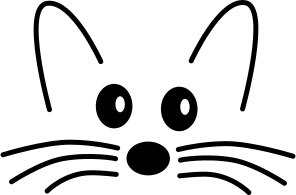
\includegraphics[width=1.4em]{squeak-logo}}}
\newcommand{\dothis}[1]{%
	\medskip
	\noindent\dothisicon
	\ifx#1\empty\else\quad\emph{#1}\fi
	\par\smallskip\nopagebreak}
% NB: To use this in an individual chapter, you must set:
%\graphicspath{{figures/} {../figures/}}
% at the head of the chapter.  Don't forget the final /
%=============================================================
%:Reader hints (hint)
%
% Indicates a non-obvious consequence 
\newcommand{\hint}[1]{\vspace{1ex}\noindent\fbox{\textsc{Astuce}} \emph{#1}}
%=================================================================
% graphics for Morphic handles
\newcommand{\grabHandle}{\raisebox{-0.2ex}{
\includegraphics[width=1em]{blackHandle}}}
\newcommand{\moveHandle}{\raisebox{-0.2ex}{
\includegraphics[width=1em]{moveHandle}}}
\newcommand{\debugHandle}{\raisebox{-0.2ex}{
\includegraphics[width=1em]{debugHandle}}}
% squeak-fr (added for Morphic handles)
\newcommand{\rotateHandle}{\raisebox{-0.2ex}{
\includegraphics[width=1em]{rotateHandle}}}
\newcommand{\viewerHandle}{\raisebox{-0.2ex}{
\includegraphics[width=1em]{viewerHandle}}}
% squeak-fr (add cloverHandle to use \clover in QuickTour.tex as alias
% todo 

%=============================================================
%:Highlighting Important stuff (doublebox)
%
% From Seaside book ...
\newsavebox{\SavedText}
\newlength{\InnerBoxRule}\setlength{\InnerBoxRule}{.75\fboxrule}
\newlength{\OuterBoxRule}\setlength{\OuterBoxRule}{1.5\fboxrule}
\newlength{\BoxSeparation}\setlength{\BoxSeparation}{1.5\fboxrule}
\addtolength{\BoxSeparation}{.5pt}
\newlength{\SaveBoxSep}\setlength{\SaveBoxSep}{2\fboxsep}
%
\newenvironment{doublebox}{\begin{lrbox}{\SavedText}
    \begin{minipage}{.75\textwidth}}
    {\end{minipage}\end{lrbox}\begin{center}
    \setlength{\fboxsep}{\BoxSeparation}\setlength{\fboxrule}{\OuterBoxRule}
    \fbox{\setlength{\fboxsep}{\SaveBoxSep}\setlength{\fboxrule}{\InnerBoxRule}%
      \fbox{\usebox{\SavedText}}}
  \end{center}}
% Use this:
\newcommand{\important}[1]{\begin{doublebox}#1\end{doublebox}}
%=============================================================
%:Section depth
\setcounter{secnumdepth}{2}
%% for this to happen start the file with
%\ifx\wholebook\relax\else
%% $Author$ Martial
% $Date$ Wed Oct 10 13:34:55 CEST 2007
% $Revision$ source: SBE 12715 
% Last Changed Date: 2007-10-08 21:32:45 +0200 (Mon, 08 Oct 2007)
%=============================================================
% NB: documentclass must be set in main document.
% Allows book to be generated in multiple formats.
%=============================================================
%:Packages
\usepackage[french]{babel}
\usepackage[T1]{fontenc}  %%%%%% really important to get the code directly in the text!
\usepackage{lmodern}
%\usepackage[scaled=0.85]{bookmanx} % needs another scale factor if used with \renewcommand{\sfdefault}{cmbr}
\usepackage{palatino}
\usepackage[scaled=0.85]{helvet}
\usepackage{microtype}
\usepackage{graphicx}
\usepackage{theorem}
\usepackage[utf8]{inputenc}
% ON: pdfsync breaks the use of p{width} for tabular columns!
\ifdefined\usepdfsync\usepackage{pdfsync}\fi % Requires texlive 2007
%=============================================================
%:More packages
%Stef should check which ones are used!
%\usepackage{picinpar}
%\usepackage{layout}
%\usepackage{color}
%\usepackage{enum}
%\usepackage{a4wide}
% \usepackage{fancyhdr}
\usepackage{ifthen}
\usepackage{float}
\usepackage{longtable}
\usepackage{makeidx}
\usepackage[nottoc]{tocbibind}
\usepackage{multicol}
\usepackage{booktabs}	% book-style tables
\usepackage{topcapt}	% enables \topcaption
\usepackage{multirow}
\usepackage{tabularx}
%\usepackage[bottom]{footmisc}
\usepackage{xspace}
\usepackage{alltt}
\usepackage{amssymb,textcomp}
\usepackage[usenames,dvipsnames]{color}
%\usepackage{colortbl}
\usepackage[hang]{subfigure}\makeatletter\def\p@subfigure{\thefigure\,}\makeatother
\usepackage{rotating}
\usepackage{enumitem}	% apb: allows more control over tags in enumerations
\usepackage{verbatim}     % for comment environment
\usepackage{varioref}	% for page references that work
\labelformat{footnote}{\thechapter--#1} % to distinguish citations from jurabib
\usepackage{needspace}
\usepackage{isodateo} % enable \isodate
\usepackage[newparttoc]{titlesec}
\usepackage{titletoc}
\usepackage{eurosym}
\usepackage{wrapfig}

\usepackage[
	super,
	citefull=first,
	authorformat={allreversed,and},
	titleformat={commasep,italic}
]{jurabib} % citations as footnotes
\usepackage[
	colorlinks=true,
	linkcolor=black,
	urlcolor=black,
	citecolor=black
]{hyperref}   % should come last

%=============================================================
%:URL style
\makeatletter

\def\url@leostyle{%
  \@ifundefined{selectfont}{\def\UrlFont{\sf}}{\def\UrlFont{\sffamily}}}
% ajouter par Martial pour \traduit (met une dague dans les \doublebox
\def\thempfootnote{\fnsymbol{mpfootnote}}

\makeatother
% Now actually use the newly defined style.
\urlstyle{leo}
%=============================================================
%:Booleans
\newboolean{lulu}
\setboolean{lulu}{false}
\newcommand{\ifluluelse}[2]{\ifthenelse{\boolean{lulu}}{#1}{#2}}
%=============================================================
%:Names
\newcommand{\SUnit}{SUnit\xspace}
\newcommand{\sunit}{SUnit\xspace}
\newcommand{\xUnit}{$x$Unit\xspace}
\newcommand{\JUnit}{JUnit\xspace}
%\newcommand{\XP}{eXtreme Programming\xspace}
\newcommand{\st}{Smalltalk\xspace}
\newcommand{\Squeak}{Squeak\xspace}
\newcommand{\sq}{Squeak\xspace}
\newcommand{\sqmap}{SqueakMap\xspace}
\newcommand{\squeak}{Squeak\xspace}
%\newcommand{\sbe}{\url{scg.unibe.ch/SBE}\xspace}
%\newcommand{\sbe}{\url{squeakbyexample.org}\xspace}
\newcommand{\sbe}{\url{SqueakByExample.org}\xspace}
% squeak-fr: adresse de la version francaise
\newcommand{\spe}{\url{SqueakByExample.org}\xspace} % ?/FR
\newcommand{\sba}{\url{SquareBracketAssociates.org}\xspace}

% squeak-fr: ajout de la \squeakdev pour eviter les problemes de
% changements d'url rencontres dans la VO:
\newcommand{\squeakdev}{\url{www.squeaksource.com/ImageForDevelopers}\xspace} %ou
%\newcommand{\squeakdev}{\url{squeak.ofset.org/squeak-dev}\xspace}

%=============================================================
%:Editorial comment macros
\newcommand{\nnbb}[2]{
    \fbox{\bfseries\sffamily\scriptsize#1}
    {\sf\small$\blacktriangleright$\textit{#2}$\blacktriangleleft$}
   }
\newcommand{\ab}[1]{\nnbb{Andrew}{#1}}
\newcommand{\sd}[1]{\nnbb{St\'{e}f}{#1}}
\newcommand{\md}[1]{\nnbb{Marcus}{#1}}
\newcommand{\on}[1]{\nnbb{Oscar}{#1}}
\newcommand{\damien}[1]{\nnbb{Damien}{#1}}
\newcommand{\lr}[1]{\nnbb{Lukas}{#1}}
\newcommand{\orla}[1]{\nnbb{Orla}{#1}}
%\newcommand{\here}{\nnbb{CONTINUE}{HERE}}
\newcommand{\here}{\nnbb{CONTINUE}{ICI}}

%=============================================================
%:Abbreviation macros
\newcommand{\ie}{\emph{c-\`a-d.}\xspace}
\newcommand{\cad}{\emph{c-\`a-d.}\xspace}
%\newcommand{\eg}{\emph{e.g.},\xspace}
\newcommand{\eg}{\emph{par ex.},\xspace}
\newcommand{\parex}{\emph{par ex.},\xspace}
\newcommand{\etc}{etc\xspace}
%=============================================================
%:Cross reference macros

% [squeak-fr] martial: remarquez les articles devant les noms
\newcommand{\charef}[1]{le chapitre~\ref{cha:#1}\xspace}
% note de martial: utilise dans chapitre Syntax.tex: a redefinir
\newcommand{\charefs}[2]{les chapitres~\ref{cha:#1} et \ref{cha:#2}\xspace}
\newcommand{\secref}[1]{la section~\ref{sec:#1}\xspace}
\newcommand{\figref}[1]{la figure~\ref{fig:#1}\xspace}
\newcommand{\Figref}[1]{La figure~\ref{fig:#1}\xspace}
\newcommand{\appref}[1]{l'annexe~\ref{app:#1}\xspace}
\newcommand{\tabref}[1]{la table~\ref{tab:#1}\xspace}
% defini pour le chapitre Messages.tex
\newcommand{\Tabref}[1]{La table~\ref{tab:#1}\xspace}

% APB: I removed trailing \xspace commands from these macros because
% \xspace mostly doesn't work.  If you want a space after your
% references, type one!
% ON: xspace has always worked just fine for me!  Please leave them in.
%
\newcommand{\ruleref}[1]{\ref{rule:#1}\xspace}
%
\newcommand{\egref}[1]{exemple~\ref{eg:#1}\xspace}
\newcommand{\Egref}[1]{Exemple~\ref{eg:#1}\xspace}
%
\newcommand{\scrref}[1]{script~\ref{scr:#1}\xspace}
\newcommand{\Scrref}[1]{Script~\ref{scr:#1}\xspace}
% t = the
\newcommand{\tscrref}[1]{le script~\ref{scr:#1}\xspace}
\newcommand{\Tscrref}[1]{Le script~\ref{scr:#1}\xspace}
%
\newcommand{\mthref}[1]{m\'ethode~\ref{mth:#1}\xspace}
\newcommand{\mthsref}[1]{m\'ethodes~\ref{mth:#1}\xspace}
\newcommand{\Mthref}[1]{M\'ethode~\ref{mth:#1}\xspace}
\newcommand{\tmthref}[1]{la m\'ethode~\ref{mth:#1}\xspace}
\newcommand{\Tmthref}[1]{La m\'ethode~\ref{mth:#1}\xspace}
%
\newcommand{\clsref}[1]{classe~\ref{cls:#1}\xspace}
\newcommand{\tclsref}[1]{la classe~\ref{cls:#1}\xspace}
\newcommand{\Tclsref}[1]{La classe~\ref{cls:#1}\xspace}
%=============================================================
%:Menu item macro
% for menu items, so we can change our minds on how to print them! (apb)
\definecolor{lightgray}{gray}{0.89}
\newcommand{\menu}[1]{{%
	\setlength{\fboxsep}{0pt}%
	\colorbox{lightgray}{{{\upshape\sffamily\strut \,#1\,}}}}}
% \newcommand{\menu}[1]{{%
% 	\fontfamily{lmr}\selectfont
% 	\upshape\textlangle{\sffamily #1}\textrangle}}
% For submenu items:
\newcommand{\go}{\,$\triangleright$\,}
% \newcommand{\go}{\,$\blacktriangleright$\,}
% For keyboard shortcuts:
%\newcommand{\short}[1]{\mbox{$\langle${\sc CMD}$\rangle$-#1}\xspace}
\newcommand{\short}[1]{\mbox{{\sc cmd}\hspace{0.08em}--\hspace{0.09em}#1}\xspace}
% For buttons:
\newcommand{\button}[1]{{%
	\setlength{\fboxsep}{0pt}%
	\fbox{{\upshape\sffamily\strut \,#1\,}}}}
\newcommand{\toolsflap}{l'onglet \textit{Tools}\xspace}
%=============================================================
%:Reader cues (do this)
%
% Indicate something the reader should try out.
\newcommand{\dothisicon}{\raisebox{-.5ex}{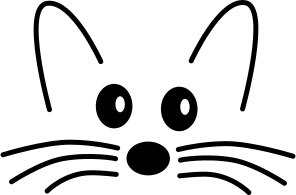
\includegraphics[width=1.4em]{squeak-logo}}}
\newcommand{\dothis}[1]{%
	\medskip
	\noindent\dothisicon
	\ifx#1\empty\else\quad\emph{#1}\fi
	\par\smallskip\nopagebreak}
% NB: To use this in an individual chapter, you must set:
%\graphicspath{{figures/} {../figures/}}
% at the head of the chapter.  Don't forget the final /
%=============================================================
%:Reader hints (hint)
%
% Indicates a non-obvious consequence 
\newcommand{\hint}[1]{\vspace{1ex}\noindent\fbox{\textsc{Astuce}} \emph{#1}}
%=================================================================
% graphics for Morphic handles
\newcommand{\grabHandle}{\raisebox{-0.2ex}{
\includegraphics[width=1em]{blackHandle}}}
\newcommand{\moveHandle}{\raisebox{-0.2ex}{
\includegraphics[width=1em]{moveHandle}}}
\newcommand{\debugHandle}{\raisebox{-0.2ex}{
\includegraphics[width=1em]{debugHandle}}}
% squeak-fr (added for Morphic handles)
\newcommand{\rotateHandle}{\raisebox{-0.2ex}{
\includegraphics[width=1em]{rotateHandle}}}
\newcommand{\viewerHandle}{\raisebox{-0.2ex}{
\includegraphics[width=1em]{viewerHandle}}}
% squeak-fr (add cloverHandle to use \clover in QuickTour.tex as alias
% todo 

%=============================================================
%:Highlighting Important stuff (doublebox)
%
% From Seaside book ...
\newsavebox{\SavedText}
\newlength{\InnerBoxRule}\setlength{\InnerBoxRule}{.75\fboxrule}
\newlength{\OuterBoxRule}\setlength{\OuterBoxRule}{1.5\fboxrule}
\newlength{\BoxSeparation}\setlength{\BoxSeparation}{1.5\fboxrule}
\addtolength{\BoxSeparation}{.5pt}
\newlength{\SaveBoxSep}\setlength{\SaveBoxSep}{2\fboxsep}
%
\newenvironment{doublebox}{\begin{lrbox}{\SavedText}
    \begin{minipage}{.75\textwidth}}
    {\end{minipage}\end{lrbox}\begin{center}
    \setlength{\fboxsep}{\BoxSeparation}\setlength{\fboxrule}{\OuterBoxRule}
    \fbox{\setlength{\fboxsep}{\SaveBoxSep}\setlength{\fboxrule}{\InnerBoxRule}%
      \fbox{\usebox{\SavedText}}}
  \end{center}}
% Use this:
\newcommand{\important}[1]{\begin{doublebox}#1\end{doublebox}}
%=============================================================
%:Section depth
\setcounter{secnumdepth}{2}
%% for this to happen start the file with
%\ifx\wholebook\relax\else
%% $Author$ Martial
% $Date$ Wed Oct 10 13:34:55 CEST 2007
% $Revision$ source: SBE 12715 
% Last Changed Date: 2007-10-08 21:32:45 +0200 (Mon, 08 Oct 2007)
%=============================================================
% NB: documentclass must be set in main document.
% Allows book to be generated in multiple formats.
%=============================================================
%:Packages
\usepackage[french]{babel}
\usepackage[T1]{fontenc}  %%%%%% really important to get the code directly in the text!
\usepackage{lmodern}
%\usepackage[scaled=0.85]{bookmanx} % needs another scale factor if used with \renewcommand{\sfdefault}{cmbr}
\usepackage{palatino}
\usepackage[scaled=0.85]{helvet}
\usepackage{microtype}
\usepackage{graphicx}
\usepackage{theorem}
\usepackage[utf8]{inputenc}
% ON: pdfsync breaks the use of p{width} for tabular columns!
\ifdefined\usepdfsync\usepackage{pdfsync}\fi % Requires texlive 2007
%=============================================================
%:More packages
%Stef should check which ones are used!
%\usepackage{picinpar}
%\usepackage{layout}
%\usepackage{color}
%\usepackage{enum}
%\usepackage{a4wide}
% \usepackage{fancyhdr}
\usepackage{ifthen}
\usepackage{float}
\usepackage{longtable}
\usepackage{makeidx}
\usepackage[nottoc]{tocbibind}
\usepackage{multicol}
\usepackage{booktabs}	% book-style tables
\usepackage{topcapt}	% enables \topcaption
\usepackage{multirow}
\usepackage{tabularx}
%\usepackage[bottom]{footmisc}
\usepackage{xspace}
\usepackage{alltt}
\usepackage{amssymb,textcomp}
\usepackage[usenames,dvipsnames]{color}
%\usepackage{colortbl}
\usepackage[hang]{subfigure}\makeatletter\def\p@subfigure{\thefigure\,}\makeatother
\usepackage{rotating}
\usepackage{enumitem}	% apb: allows more control over tags in enumerations
\usepackage{verbatim}     % for comment environment
\usepackage{varioref}	% for page references that work
\labelformat{footnote}{\thechapter--#1} % to distinguish citations from jurabib
\usepackage{needspace}
\usepackage{isodateo} % enable \isodate
\usepackage[newparttoc]{titlesec}
\usepackage{titletoc}
\usepackage{eurosym}
\usepackage{wrapfig}

\usepackage[
	super,
	citefull=first,
	authorformat={allreversed,and},
	titleformat={commasep,italic}
]{jurabib} % citations as footnotes
\usepackage[
	colorlinks=true,
	linkcolor=black,
	urlcolor=black,
	citecolor=black
]{hyperref}   % should come last

%=============================================================
%:URL style
\makeatletter

\def\url@leostyle{%
  \@ifundefined{selectfont}{\def\UrlFont{\sf}}{\def\UrlFont{\sffamily}}}
% ajouter par Martial pour \traduit (met une dague dans les \doublebox
\def\thempfootnote{\fnsymbol{mpfootnote}}

\makeatother
% Now actually use the newly defined style.
\urlstyle{leo}
%=============================================================
%:Booleans
\newboolean{lulu}
\setboolean{lulu}{false}
\newcommand{\ifluluelse}[2]{\ifthenelse{\boolean{lulu}}{#1}{#2}}
%=============================================================
%:Names
\newcommand{\SUnit}{SUnit\xspace}
\newcommand{\sunit}{SUnit\xspace}
\newcommand{\xUnit}{$x$Unit\xspace}
\newcommand{\JUnit}{JUnit\xspace}
%\newcommand{\XP}{eXtreme Programming\xspace}
\newcommand{\st}{Smalltalk\xspace}
\newcommand{\Squeak}{Squeak\xspace}
\newcommand{\sq}{Squeak\xspace}
\newcommand{\sqmap}{SqueakMap\xspace}
\newcommand{\squeak}{Squeak\xspace}
%\newcommand{\sbe}{\url{scg.unibe.ch/SBE}\xspace}
%\newcommand{\sbe}{\url{squeakbyexample.org}\xspace}
\newcommand{\sbe}{\url{SqueakByExample.org}\xspace}
% squeak-fr: adresse de la version francaise
\newcommand{\spe}{\url{SqueakByExample.org}\xspace} % ?/FR
\newcommand{\sba}{\url{SquareBracketAssociates.org}\xspace}

% squeak-fr: ajout de la \squeakdev pour eviter les problemes de
% changements d'url rencontres dans la VO:
\newcommand{\squeakdev}{\url{www.squeaksource.com/ImageForDevelopers}\xspace} %ou
%\newcommand{\squeakdev}{\url{squeak.ofset.org/squeak-dev}\xspace}

%=============================================================
%:Editorial comment macros
\newcommand{\nnbb}[2]{
    \fbox{\bfseries\sffamily\scriptsize#1}
    {\sf\small$\blacktriangleright$\textit{#2}$\blacktriangleleft$}
   }
\newcommand{\ab}[1]{\nnbb{Andrew}{#1}}
\newcommand{\sd}[1]{\nnbb{St\'{e}f}{#1}}
\newcommand{\md}[1]{\nnbb{Marcus}{#1}}
\newcommand{\on}[1]{\nnbb{Oscar}{#1}}
\newcommand{\damien}[1]{\nnbb{Damien}{#1}}
\newcommand{\lr}[1]{\nnbb{Lukas}{#1}}
\newcommand{\orla}[1]{\nnbb{Orla}{#1}}
%\newcommand{\here}{\nnbb{CONTINUE}{HERE}}
\newcommand{\here}{\nnbb{CONTINUE}{ICI}}

%=============================================================
%:Abbreviation macros
\newcommand{\ie}{\emph{c-\`a-d.}\xspace}
\newcommand{\cad}{\emph{c-\`a-d.}\xspace}
%\newcommand{\eg}{\emph{e.g.},\xspace}
\newcommand{\eg}{\emph{par ex.},\xspace}
\newcommand{\parex}{\emph{par ex.},\xspace}
\newcommand{\etc}{etc\xspace}
%=============================================================
%:Cross reference macros

% [squeak-fr] martial: remarquez les articles devant les noms
\newcommand{\charef}[1]{le chapitre~\ref{cha:#1}\xspace}
% note de martial: utilise dans chapitre Syntax.tex: a redefinir
\newcommand{\charefs}[2]{les chapitres~\ref{cha:#1} et \ref{cha:#2}\xspace}
\newcommand{\secref}[1]{la section~\ref{sec:#1}\xspace}
\newcommand{\figref}[1]{la figure~\ref{fig:#1}\xspace}
\newcommand{\Figref}[1]{La figure~\ref{fig:#1}\xspace}
\newcommand{\appref}[1]{l'annexe~\ref{app:#1}\xspace}
\newcommand{\tabref}[1]{la table~\ref{tab:#1}\xspace}
% defini pour le chapitre Messages.tex
\newcommand{\Tabref}[1]{La table~\ref{tab:#1}\xspace}

% APB: I removed trailing \xspace commands from these macros because
% \xspace mostly doesn't work.  If you want a space after your
% references, type one!
% ON: xspace has always worked just fine for me!  Please leave them in.
%
\newcommand{\ruleref}[1]{\ref{rule:#1}\xspace}
%
\newcommand{\egref}[1]{exemple~\ref{eg:#1}\xspace}
\newcommand{\Egref}[1]{Exemple~\ref{eg:#1}\xspace}
%
\newcommand{\scrref}[1]{script~\ref{scr:#1}\xspace}
\newcommand{\Scrref}[1]{Script~\ref{scr:#1}\xspace}
% t = the
\newcommand{\tscrref}[1]{le script~\ref{scr:#1}\xspace}
\newcommand{\Tscrref}[1]{Le script~\ref{scr:#1}\xspace}
%
\newcommand{\mthref}[1]{m\'ethode~\ref{mth:#1}\xspace}
\newcommand{\mthsref}[1]{m\'ethodes~\ref{mth:#1}\xspace}
\newcommand{\Mthref}[1]{M\'ethode~\ref{mth:#1}\xspace}
\newcommand{\tmthref}[1]{la m\'ethode~\ref{mth:#1}\xspace}
\newcommand{\Tmthref}[1]{La m\'ethode~\ref{mth:#1}\xspace}
%
\newcommand{\clsref}[1]{classe~\ref{cls:#1}\xspace}
\newcommand{\tclsref}[1]{la classe~\ref{cls:#1}\xspace}
\newcommand{\Tclsref}[1]{La classe~\ref{cls:#1}\xspace}
%=============================================================
%:Menu item macro
% for menu items, so we can change our minds on how to print them! (apb)
\definecolor{lightgray}{gray}{0.89}
\newcommand{\menu}[1]{{%
	\setlength{\fboxsep}{0pt}%
	\colorbox{lightgray}{{{\upshape\sffamily\strut \,#1\,}}}}}
% \newcommand{\menu}[1]{{%
% 	\fontfamily{lmr}\selectfont
% 	\upshape\textlangle{\sffamily #1}\textrangle}}
% For submenu items:
\newcommand{\go}{\,$\triangleright$\,}
% \newcommand{\go}{\,$\blacktriangleright$\,}
% For keyboard shortcuts:
%\newcommand{\short}[1]{\mbox{$\langle${\sc CMD}$\rangle$-#1}\xspace}
\newcommand{\short}[1]{\mbox{{\sc cmd}\hspace{0.08em}--\hspace{0.09em}#1}\xspace}
% For buttons:
\newcommand{\button}[1]{{%
	\setlength{\fboxsep}{0pt}%
	\fbox{{\upshape\sffamily\strut \,#1\,}}}}
\newcommand{\toolsflap}{l'onglet \textit{Tools}\xspace}
%=============================================================
%:Reader cues (do this)
%
% Indicate something the reader should try out.
\newcommand{\dothisicon}{\raisebox{-.5ex}{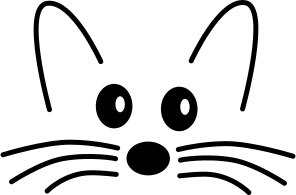
\includegraphics[width=1.4em]{squeak-logo}}}
\newcommand{\dothis}[1]{%
	\medskip
	\noindent\dothisicon
	\ifx#1\empty\else\quad\emph{#1}\fi
	\par\smallskip\nopagebreak}
% NB: To use this in an individual chapter, you must set:
%\graphicspath{{figures/} {../figures/}}
% at the head of the chapter.  Don't forget the final /
%=============================================================
%:Reader hints (hint)
%
% Indicates a non-obvious consequence 
\newcommand{\hint}[1]{\vspace{1ex}\noindent\fbox{\textsc{Astuce}} \emph{#1}}
%=================================================================
% graphics for Morphic handles
\newcommand{\grabHandle}{\raisebox{-0.2ex}{
\includegraphics[width=1em]{blackHandle}}}
\newcommand{\moveHandle}{\raisebox{-0.2ex}{
\includegraphics[width=1em]{moveHandle}}}
\newcommand{\debugHandle}{\raisebox{-0.2ex}{
\includegraphics[width=1em]{debugHandle}}}
% squeak-fr (added for Morphic handles)
\newcommand{\rotateHandle}{\raisebox{-0.2ex}{
\includegraphics[width=1em]{rotateHandle}}}
\newcommand{\viewerHandle}{\raisebox{-0.2ex}{
\includegraphics[width=1em]{viewerHandle}}}
% squeak-fr (add cloverHandle to use \clover in QuickTour.tex as alias
% todo 

%=============================================================
%:Highlighting Important stuff (doublebox)
%
% From Seaside book ...
\newsavebox{\SavedText}
\newlength{\InnerBoxRule}\setlength{\InnerBoxRule}{.75\fboxrule}
\newlength{\OuterBoxRule}\setlength{\OuterBoxRule}{1.5\fboxrule}
\newlength{\BoxSeparation}\setlength{\BoxSeparation}{1.5\fboxrule}
\addtolength{\BoxSeparation}{.5pt}
\newlength{\SaveBoxSep}\setlength{\SaveBoxSep}{2\fboxsep}
%
\newenvironment{doublebox}{\begin{lrbox}{\SavedText}
    \begin{minipage}{.75\textwidth}}
    {\end{minipage}\end{lrbox}\begin{center}
    \setlength{\fboxsep}{\BoxSeparation}\setlength{\fboxrule}{\OuterBoxRule}
    \fbox{\setlength{\fboxsep}{\SaveBoxSep}\setlength{\fboxrule}{\InnerBoxRule}%
      \fbox{\usebox{\SavedText}}}
  \end{center}}
% Use this:
\newcommand{\important}[1]{\begin{doublebox}#1\end{doublebox}}
%=============================================================
%:Section depth
\setcounter{secnumdepth}{2}
%% for this to happen start the file with
%\ifx\wholebook\relax\else
%\input{../common.tex}
%\begin{document}
%\fi
% and terminate by
% \ifx\wholebook\relax\else\end{document}\fi

\DeclareGraphicsExtensions{.pdf, .jpg, .png}
%=============================================================
%:PDF setup
\hypersetup{
%   a4paper,
%   pdfstartview=FitV,
%   colorlinks,
%   linkcolor=darkblue,
%   citecolor=darkblue,
%   pdftitle={Squeak by Example},
pdftitle={Squeak par l'exemple},
   pdfauthor={Andrew Black, St\'ephane Ducasse,	Oscar Nierstrasz,
Damien Pollet},
   pdfkeywords={Smalltalk, Squeak, Programmation Orient\'ee Objet},
pdfsubject={Informatique, Computer Science}
}
%=============================================================
%:Page layout and appearance
%
% \renewcommand{\headrulewidth}{0pt}
\renewcommand{\chaptermark}[1]{\markboth{#1}{}}
\renewcommand{\sectionmark}[1]{\markright{\thesection\ #1}}
\renewpagestyle{plain}[\small\itshape]{%
	\setheadrule{0pt}%
	\sethead[\thepage][][]{}{}{\thepage}%
	\setfoot[][][]{}{}{}}
\renewpagestyle{headings}[\small\itshape]{%
	\setheadrule{0pt}%
	\setmarks{chapter}{section}%
	\sethead[\thepage][][\chaptertitle]{\sectiontitle}{}{\thepage}%
	\setfoot[][][]{}{}{}}
%=============================================================
%:Title section setup and TOC numbering depth
\setcounter{secnumdepth}{1}
\setcounter{tocdepth}{1}
\titleformat{\part}[display]{\centering}{\huge\partname\ \thepart}{1em}{\Huge\textbf}[]
\titleformat{\chapter}[display]{}{\huge\chaptertitlename\ \thechapter}{1em}{\Huge\raggedright\textbf}[]
\titlecontents{part}[3pc]{%
		\pagebreak[2]\addvspace{1em plus.4em minus.2em}%
		\leavevmode\large\bfseries}
	{\contentslabel{3pc}}{\hspace*{-3pc}}
	{}[\nopagebreak]
\titlecontents{chapter}[3pc]{%
		\pagebreak[0]\addvspace{1em plus.2em minus.2em}%
		\leavevmode\bfseries}
	{\contentslabel{3pc}}{}
	{\hfill\contentspage}[\nopagebreak]
\dottedcontents{section}[3pc]{}{3pc}{1pc}
\dottedcontents{subsection}[3pc]{}{0pc}{1pc}
% \dottedcontents{subsection}[4.5em]{}{0pt}{1pc}
% Make \cleardoublepage insert really blank pages http://www.tex.ac.uk/cgi-bin/texfaq2html?label=reallyblank
\let\origdoublepage\cleardoublepage
\newcommand{\clearemptydoublepage}{%
  \clearpage
  {\pagestyle{empty}\origdoublepage}}
\let\cleardoublepage\clearemptydoublepage % see http://www.tex.ac.uk/cgi-bin/texfaq2html?label=patch
%=============================================================
%:FAQ macros (for FAQ chapter)
\newtheorem{faq}{FAQ}
\newcommand{\answer}{\paragraph{R\'eponse}\ }
%=============================================================
%:Listings package configuration
\usepackage{listings}
\newcommand{\caret}{\makebox{\raisebox{0.4ex}{\footnotesize{$\wedge$}}}}
\lstdefinelanguage{Smalltalk}{
%  morekeywords={self,super,true,false,nil,thisContext}, % This is overkill
  morestring=[d]',
  morecomment=[s]{"}{"},
  alsoletter={\#:},
  escapechar={!},
  escapebegin=\itshape, % comment-like by default (Martial 11/2007)
  literate=
    {BANG}{!}1
    {UNDERSCORE}{\_}1
    {\\st}{Smalltalk}9 % convenience -- in case \st occurs in code
    % {'}{{\textquotesingle}}1 % replaced by upquote=true in \lstset
    {_}{{$\leftarrow$}}1
    {>>>}{{\sep}}1
    {^}{{$\uparrow$}}1
    {~}{{$\sim$}}1
    {-}{{\sf -\hspace{-0.13em}-}}1  % the goal is to make - the same width as +
    {+}{\raisebox{0.08ex}{+}}1		% and to raise + off the baseline to match -
    {-->}{{\quad$\longrightarrow$\quad}}3
	, % Don't forget the comma at the end!
  tabsize=4
}[keywords,comments,strings]
% ajout pour les échappements dans les codes
% indispensable pour mettre le code en emphase (cf. Model.tex) 
\newcommand{\codeify}[1]{\NoAutoSpaceBeforeFDP#1\AutoSpaceBeforeFDP}
\newcommand{\normcomment}[1]{\emph{#1}} %cf. Streams
\newcommand{\normcode}[1]{\emph{\codeify{#1}}} %cf. Streams
\newcommand{\emcode}[1]{\textbf{\normcode{#1}}} % Martial 11/2007
\lstset{language=Smalltalk,
	basicstyle=\sffamily,
	keywordstyle=\color{black}\bfseries,
	% stringstyle=\ttfamily, % Ugly! do we really want this? -- on
	%commentstyle=\itshape,
	mathescape=true,
	showstringspaces=false,
	keepspaces=true,
	breaklines=true,
	breakautoindent=true,
	lineskip={-1pt}, % Ugly hack
	upquote=true, % straight quote; requires textcomp package
	columns=fullflexible} % no fixed width fonts
% In-line code (literal)
% Normally use this for all in-line code:
\newcommand{\ct}{\lstinline[mathescape=false,basicstyle={\sffamily\upshape}]}
% apb 2007.8.28 added the \upshape declaration to avoid getting italicized code in \dothis{ } sections.
% In-line code (latex enabled)
% Use this only in special situations where \ct does not work
% (within section headings ...):

% [squeak-fr] Modification de \lct suivant les indications de Martial Boniou
\newcommand{\lct}[1]{\textsf{\textup{\NoAutoSpaceBeforeFDP #1
\AutoSpaceBeforeFDP}}} %\xspace

% Use these for system categories and protocols:
\newcommand{\scat}[1]{\emph{\textsf{#1}}\xspace}
\newcommand{\pkg}[1]{\emph{\textsf{#1}}\xspace}
\newcommand{\prot}[1]{\emph{\textsf{#1}}\xspace}
% Code environments
% NB: the arg is for tests
% Only code and example environments may be tests
\lstnewenvironment{code}[1]{%
	\lstset{%
		frame=lines,
		mathescape=false
	}
}{}
\def\ignoredollar#1{}
%=============================================================
%:Code environments (method, script ...)
% NB: the third arg is for tests
% Only code and example environments may be tests
\lstnewenvironment{example}[3][defaultlabel]{%
	\renewcommand{\lstlistingname}{Exemple}%
	\lstset{
		frame=lines,
		mathescape=false,
		caption={\emph{#2}},
		label={eg:#1}
	}
}{}
\lstnewenvironment{script}[2][defaultlabel]{%
\renewcommand{\lstlistingname}{Script}%
	\lstset{
		frame=lines,
		mathescape=false,
		name={Script},
		caption={\emph{#2}},
		label={scr:#1}
	}
}{}
\lstnewenvironment{method}[2][defaultlabel]{%
	\renewcommand{\lstlistingname}{M\'ethode}%
	\lstset{
		frame=lines,
		mathescape=false,
		name={M\'ethode},
		caption={\emph{#2}},
		label={mth:#1}
	}
}{}
\lstnewenvironment{methods}[2][defaultlabel]{% just for multiple methods at once
	\renewcommand{\lstlistingname}{M\'ethodes}%
	\lstset{
		frame=lines,
		mathescape=false,
		name={M\'ethode},
		caption={\emph{#2}},
		label={mth:#1}
	}
}{}
\lstnewenvironment{numMethod}[2][defaultlabel]{%
	\renewcommand{\lstlistingname}{M\'ethode}%
	\lstset{
		numbers=left,
		numberstyle={\tiny\sffamily},
		frame=lines,
		mathescape=false,
		name={M\'ethode},
		caption={\emph{#2}},
		label={mth:#1}
	}
}{}
\lstnewenvironment{classdef}[2][defaultlabel]{%
	\renewcommand{\lstlistingname}{Classe}%
	\lstset{
		frame=lines,
		mathescape=false,
		name={Classe},
		caption={\emph{#2}},
		label={cls:#1}
	}
}{}
%=============================================================
%:Reserving space
% Usually need one more line than the actual lines of code
\newcommand{\needlines}[1]{\Needspace{#1\baselineskip}}
%=============================================================
%:Indexing macros
% Macros ending with "ind" generate text as well as an index entry
% Macros ending with "index" *only* generate an index entry
\newcommand{\ind}[1]{\index{#1}#1\xspace} % plain text
\newcommand{\subind}[2]{\index{#1!#2}#2\xspace} % show #2, subindex inder #1
\newcommand{\emphind}[1]{\index{#1}\emph{#1}\xspace} % emph #1
\newcommand{\emphsubind}[2]{\index{#1!#2}\emph{#2}\xspace} % show emph #2, subindex inder #1
\newcommand{\scatind}[1]{\index{#1@\textsf{#1} (cat\'egorie)}\scat{#1}} % category
\newcommand{\protind}[1]{\index{#1@\textsf{#1} (protocole)}\prot{#1}} % protocol
% \newcommand{\clsind}[1]{\index{#1@\textsf{#1} (class)}\ct{#1}\xspace}
\newcommand{\clsind}[1]{\index{#1!\#@(classe)}\ct{#1}\xspace} % class
\newcommand{\cvind}[1]{\index{#1@\textsf{#1} (variable de classe)}\ct{#1}\xspace} % class var
\newcommand{\glbind}[1]{\index{#1@\textsf{#1} (globale)}\ct{#1}\xspace} % global
\newcommand{\patind}[1]{\index{#1@#1 (patron)}\ct{#1}\xspace} % pattern
\newcommand{\pvind}[1]{\index{#1@\textsf{#1} (pseudo-variable)}\ct{#1}\xspace} % pseudo variable
% [squeak - fr]Martial: I found the following cleaner (should be
% merged in SBE for self and super)
\newcommand{\subpvindex}[2]{\index{#1@\textsf{#1} (pseudo-variable)!#2}}
\newcommand{\subpvind}[2]{\index{#1@\textsf{#1} (pseudo-variable)!#2}#2\xspace}
% used in Model.tex
\newcommand{\mthind}[2]{\index{#1!#2@\ct{#2}}\ct{#2}\xspace} % show method name only
\newcommand{\lmthind}[2]{\index{#1!#2@\ct{#2}}\lct{#2}\xspace} % show method name only
\newcommand{\cmind}[2]{\index{#1!#2@\ct{#2}}\ct{#1>>>#2}\xspace} % show class>>method
\newcommand{\toolsflapind}{\index{onglet Tools}\toolsflap} % index tools flap
% The following only generate an index entry:
% \newcommand{\clsindex}[1]{\index{#1@\textsf{#1} (class)}}
\newcommand{\clsindex}[1]{\index{#1!\#@(classe)}} % class
\newcommand{\cmindex}[2]{\index{#1!#2@\ct{#2}}} % class>>method
\newcommand{\cvindex}[1]{\index{#1@\textsf{#1} (variable de classe)}} % class var
\newcommand{\glbindex}[1]{\index{#1@\textsf{#1} (globale)}}% global
\newcommand{\pvindex}[1]{\index{#1@\textsf{#1} (pseudo-variable)}}% pseudo var
\newcommand{\seeindex}[2]{\index{#1|see{#2}}} % #1, see #2
\newcommand{\scatindex}[1]{\index{#1@\textsf{#1} (cat\'egorie)}} % category
\newcommand{\protindex}[1]{\index{#1@\textsf{#1} (protocole)}} % protocol
% How can we have the main entry page numbers in bold yet not break the hyperlink?
\newcommand{\boldidx}[1]{{\bf #1}} % breaks hyperlink
%\newcommand{\indmain}[1]{\index{#1|boldidx}#1\xspace} % plain text, main entry
%\newcommand{\emphsubindmain}[2]{\index{#1!#2|boldidx}\emph{#2}\xspace} % subindex, main entry
%\newcommand{\subindmain}[2]{\index{#1!#2|boldidx}#2\xspace} % subindex, main entry
%\newcommand{\clsindmain}[1]{\index{#1@\textsf{#1} (class)|boldidx}\ct{#1}\xspace}
%\newcommand{\clsindmain}[1]{\index{#1!\#@(class)|boldidx}\ct{#1}\xspace} % class main
%\newcommand{\indexmain}[1]{\index{#1|boldidx}} % main index entry only
\newcommand{\indmain}[1]{\index{#1}#1\xspace} 
\newcommand{\emphsubindmain}[2]{\index{#1!#2}\emph{#2}\xspace} % subindex, main entry
\newcommand{\subindmain}[2]{\index{#1!#2}#2\xspace} % subindex, main entry
%\newcommand{\clsindmain}[1]{\index{#1@\textsf{#1} (class)}\ct{#1}\xspace}
\newcommand{\clsindmain}[1]{\index{#1!\#@(classe)}\ct{#1}\xspace} % class main
\newcommand{\indexmain}[1]{\index{#1}} 
%=============================================================
%:Code macros
% some constants
\newcommand{\codesize}{\small}
\newcommand{\codefont}{\sffamily}
\newcommand{\cat}[1]{\textit{Dans la cat\'egorie #1}}%%To remove later
\newlength{\scriptindent}
\setlength{\scriptindent}{.3cm}
%% Method presentation constants
\newlength{\methodindent}
\newlength{\methodwordlength}
\newlength{\aftermethod}
\setlength{\methodindent}{0.2cm}
\settowidth{\methodwordlength}{\ M\'ethode\ }
%=============================================================
%:Smalltalk macros
%\newcommand{\sep}{{$\gg$}}
\newcommand{\sep}{\mbox{>>}}
\newcommand{\self}{\ct{self}\xspace}
\newcommand{\super}{\ct{super}\xspace}
\newcommand{\nil}{\ct{nil}\xspace}
%=============================================================
% be less conservative about float placement
% these commands are from http://www.tex.ac.uk/cgi-bin/texfaq2html?label=floats
\renewcommand{\topfraction}{.9}
\renewcommand{\bottomfraction}{.9}
\renewcommand{\textfraction}{.1}
\renewcommand{\floatpagefraction}{.85}
\renewcommand{\dbltopfraction}{.66}
\renewcommand{\dblfloatpagefraction}{.85}
\setcounter{topnumber}{9}
\setcounter{bottomnumber}{9}
\setcounter{totalnumber}{20}
\setcounter{dbltopnumber}{9}
%=============================================================
%% [Squeak-fr]
% pour identifier les zones de texte à corriger d'urgence!
\newcommand{\arevoir}[1]{#1}
% \traduit utilisé dans Model.tex
\newcommand{\traduit}[1]{\footnote[2]{#1}}
% changeset alias
\newcommand{\changeset}{\emph{change set}\xspace}
\newcommand{\changesets}{\emph{change sets}\xspace}
% callback alias
\newcommand{\callback}{\emph{callback}\xspace}
% blobmorph alias (QuickTour->blob)
\newcommand{\blobmorph}{\emph{blob}\xspace}
% repository
\newcommand{\squeaksource}{\textsf{SqueakSource}\xspace}
\newcommand{\sourceforge}{\textsf{SourceForge}\xspace}
% L'onglet Tools
\newcommand{\Toolsflap}{L'onglet \textit{Tools}\xspace}
% Mac OS X
\newcommand{\macosx}{\mbox{Mac OS X}\xspace}
% code en francais (uniquement dans le chapitre BasicClasses)
\newcommand{\codefrench}[1]{\NoAutoSpaceBeforeFDP\texttt{#1}\AutoSpaceBeforeFDP\xspace}
% mantra du modele objet (suite a l'erreur de martial)
\newcommand{\Mantra}{Tout est objet\xspace}
\newcommand{\mantra}{\MakeLowercase{\Mantra}\xspace}
% césure
\hyphenation{Omni-Brow-ser}
\hyphenation{m\'e-tho-de} % erreur de cesure commune
\hyphenation{m\'e-tho-des}
\hyphenation{e-xem-ple}
\hyphenation{en-re-gi-stre}
\hyphenation{a-na-ly-seur}
\hyphenation{glo-ba-le}
\hyphenation{fi-gu-re}
\hyphenation{vi-si-bles}
\hyphenation{cor-res-pon-dan-te}
\hyphenation{Work-space}
%=============================================================
% apb doesn't like paragraphs to run in to each other without a break
\parskip 1ex
%=============================================================
%:Stuff to check, merge or deprecate
%\setlength{\marginparsep}{2mm}
%\renewcommand{\baselinestretch}{1.1}
%=============================================================

%\begin{document}
%\fi
% and terminate by
% \ifx\wholebook\relax\else\end{document}\fi

\DeclareGraphicsExtensions{.pdf, .jpg, .png}
%=============================================================
%:PDF setup
\hypersetup{
%   a4paper,
%   pdfstartview=FitV,
%   colorlinks,
%   linkcolor=darkblue,
%   citecolor=darkblue,
%   pdftitle={Squeak by Example},
pdftitle={Squeak par l'exemple},
   pdfauthor={Andrew Black, St\'ephane Ducasse,	Oscar Nierstrasz,
Damien Pollet},
   pdfkeywords={Smalltalk, Squeak, Programmation Orient\'ee Objet},
pdfsubject={Informatique, Computer Science}
}
%=============================================================
%:Page layout and appearance
%
% \renewcommand{\headrulewidth}{0pt}
\renewcommand{\chaptermark}[1]{\markboth{#1}{}}
\renewcommand{\sectionmark}[1]{\markright{\thesection\ #1}}
\renewpagestyle{plain}[\small\itshape]{%
	\setheadrule{0pt}%
	\sethead[\thepage][][]{}{}{\thepage}%
	\setfoot[][][]{}{}{}}
\renewpagestyle{headings}[\small\itshape]{%
	\setheadrule{0pt}%
	\setmarks{chapter}{section}%
	\sethead[\thepage][][\chaptertitle]{\sectiontitle}{}{\thepage}%
	\setfoot[][][]{}{}{}}
%=============================================================
%:Title section setup and TOC numbering depth
\setcounter{secnumdepth}{1}
\setcounter{tocdepth}{1}
\titleformat{\part}[display]{\centering}{\huge\partname\ \thepart}{1em}{\Huge\textbf}[]
\titleformat{\chapter}[display]{}{\huge\chaptertitlename\ \thechapter}{1em}{\Huge\raggedright\textbf}[]
\titlecontents{part}[3pc]{%
		\pagebreak[2]\addvspace{1em plus.4em minus.2em}%
		\leavevmode\large\bfseries}
	{\contentslabel{3pc}}{\hspace*{-3pc}}
	{}[\nopagebreak]
\titlecontents{chapter}[3pc]{%
		\pagebreak[0]\addvspace{1em plus.2em minus.2em}%
		\leavevmode\bfseries}
	{\contentslabel{3pc}}{}
	{\hfill\contentspage}[\nopagebreak]
\dottedcontents{section}[3pc]{}{3pc}{1pc}
\dottedcontents{subsection}[3pc]{}{0pc}{1pc}
% \dottedcontents{subsection}[4.5em]{}{0pt}{1pc}
% Make \cleardoublepage insert really blank pages http://www.tex.ac.uk/cgi-bin/texfaq2html?label=reallyblank
\let\origdoublepage\cleardoublepage
\newcommand{\clearemptydoublepage}{%
  \clearpage
  {\pagestyle{empty}\origdoublepage}}
\let\cleardoublepage\clearemptydoublepage % see http://www.tex.ac.uk/cgi-bin/texfaq2html?label=patch
%=============================================================
%:FAQ macros (for FAQ chapter)
\newtheorem{faq}{FAQ}
\newcommand{\answer}{\paragraph{R\'eponse}\ }
%=============================================================
%:Listings package configuration
\usepackage{listings}
\newcommand{\caret}{\makebox{\raisebox{0.4ex}{\footnotesize{$\wedge$}}}}
\lstdefinelanguage{Smalltalk}{
%  morekeywords={self,super,true,false,nil,thisContext}, % This is overkill
  morestring=[d]',
  morecomment=[s]{"}{"},
  alsoletter={\#:},
  escapechar={!},
  escapebegin=\itshape, % comment-like by default (Martial 11/2007)
  literate=
    {BANG}{!}1
    {UNDERSCORE}{\_}1
    {\\st}{Smalltalk}9 % convenience -- in case \st occurs in code
    % {'}{{\textquotesingle}}1 % replaced by upquote=true in \lstset
    {_}{{$\leftarrow$}}1
    {>>>}{{\sep}}1
    {^}{{$\uparrow$}}1
    {~}{{$\sim$}}1
    {-}{{\sf -\hspace{-0.13em}-}}1  % the goal is to make - the same width as +
    {+}{\raisebox{0.08ex}{+}}1		% and to raise + off the baseline to match -
    {-->}{{\quad$\longrightarrow$\quad}}3
	, % Don't forget the comma at the end!
  tabsize=4
}[keywords,comments,strings]
% ajout pour les échappements dans les codes
% indispensable pour mettre le code en emphase (cf. Model.tex) 
\newcommand{\codeify}[1]{\NoAutoSpaceBeforeFDP#1\AutoSpaceBeforeFDP}
\newcommand{\normcomment}[1]{\emph{#1}} %cf. Streams
\newcommand{\normcode}[1]{\emph{\codeify{#1}}} %cf. Streams
\newcommand{\emcode}[1]{\textbf{\normcode{#1}}} % Martial 11/2007
\lstset{language=Smalltalk,
	basicstyle=\sffamily,
	keywordstyle=\color{black}\bfseries,
	% stringstyle=\ttfamily, % Ugly! do we really want this? -- on
	%commentstyle=\itshape,
	mathescape=true,
	showstringspaces=false,
	keepspaces=true,
	breaklines=true,
	breakautoindent=true,
	lineskip={-1pt}, % Ugly hack
	upquote=true, % straight quote; requires textcomp package
	columns=fullflexible} % no fixed width fonts
% In-line code (literal)
% Normally use this for all in-line code:
\newcommand{\ct}{\lstinline[mathescape=false,basicstyle={\sffamily\upshape}]}
% apb 2007.8.28 added the \upshape declaration to avoid getting italicized code in \dothis{ } sections.
% In-line code (latex enabled)
% Use this only in special situations where \ct does not work
% (within section headings ...):

% [squeak-fr] Modification de \lct suivant les indications de Martial Boniou
\newcommand{\lct}[1]{\textsf{\textup{\NoAutoSpaceBeforeFDP #1
\AutoSpaceBeforeFDP}}} %\xspace

% Use these for system categories and protocols:
\newcommand{\scat}[1]{\emph{\textsf{#1}}\xspace}
\newcommand{\pkg}[1]{\emph{\textsf{#1}}\xspace}
\newcommand{\prot}[1]{\emph{\textsf{#1}}\xspace}
% Code environments
% NB: the arg is for tests
% Only code and example environments may be tests
\lstnewenvironment{code}[1]{%
	\lstset{%
		frame=lines,
		mathescape=false
	}
}{}
\def\ignoredollar#1{}
%=============================================================
%:Code environments (method, script ...)
% NB: the third arg is for tests
% Only code and example environments may be tests
\lstnewenvironment{example}[3][defaultlabel]{%
	\renewcommand{\lstlistingname}{Exemple}%
	\lstset{
		frame=lines,
		mathescape=false,
		caption={\emph{#2}},
		label={eg:#1}
	}
}{}
\lstnewenvironment{script}[2][defaultlabel]{%
\renewcommand{\lstlistingname}{Script}%
	\lstset{
		frame=lines,
		mathescape=false,
		name={Script},
		caption={\emph{#2}},
		label={scr:#1}
	}
}{}
\lstnewenvironment{method}[2][defaultlabel]{%
	\renewcommand{\lstlistingname}{M\'ethode}%
	\lstset{
		frame=lines,
		mathescape=false,
		name={M\'ethode},
		caption={\emph{#2}},
		label={mth:#1}
	}
}{}
\lstnewenvironment{methods}[2][defaultlabel]{% just for multiple methods at once
	\renewcommand{\lstlistingname}{M\'ethodes}%
	\lstset{
		frame=lines,
		mathescape=false,
		name={M\'ethode},
		caption={\emph{#2}},
		label={mth:#1}
	}
}{}
\lstnewenvironment{numMethod}[2][defaultlabel]{%
	\renewcommand{\lstlistingname}{M\'ethode}%
	\lstset{
		numbers=left,
		numberstyle={\tiny\sffamily},
		frame=lines,
		mathescape=false,
		name={M\'ethode},
		caption={\emph{#2}},
		label={mth:#1}
	}
}{}
\lstnewenvironment{classdef}[2][defaultlabel]{%
	\renewcommand{\lstlistingname}{Classe}%
	\lstset{
		frame=lines,
		mathescape=false,
		name={Classe},
		caption={\emph{#2}},
		label={cls:#1}
	}
}{}
%=============================================================
%:Reserving space
% Usually need one more line than the actual lines of code
\newcommand{\needlines}[1]{\Needspace{#1\baselineskip}}
%=============================================================
%:Indexing macros
% Macros ending with "ind" generate text as well as an index entry
% Macros ending with "index" *only* generate an index entry
\newcommand{\ind}[1]{\index{#1}#1\xspace} % plain text
\newcommand{\subind}[2]{\index{#1!#2}#2\xspace} % show #2, subindex inder #1
\newcommand{\emphind}[1]{\index{#1}\emph{#1}\xspace} % emph #1
\newcommand{\emphsubind}[2]{\index{#1!#2}\emph{#2}\xspace} % show emph #2, subindex inder #1
\newcommand{\scatind}[1]{\index{#1@\textsf{#1} (cat\'egorie)}\scat{#1}} % category
\newcommand{\protind}[1]{\index{#1@\textsf{#1} (protocole)}\prot{#1}} % protocol
% \newcommand{\clsind}[1]{\index{#1@\textsf{#1} (class)}\ct{#1}\xspace}
\newcommand{\clsind}[1]{\index{#1!\#@(classe)}\ct{#1}\xspace} % class
\newcommand{\cvind}[1]{\index{#1@\textsf{#1} (variable de classe)}\ct{#1}\xspace} % class var
\newcommand{\glbind}[1]{\index{#1@\textsf{#1} (globale)}\ct{#1}\xspace} % global
\newcommand{\patind}[1]{\index{#1@#1 (patron)}\ct{#1}\xspace} % pattern
\newcommand{\pvind}[1]{\index{#1@\textsf{#1} (pseudo-variable)}\ct{#1}\xspace} % pseudo variable
% [squeak - fr]Martial: I found the following cleaner (should be
% merged in SBE for self and super)
\newcommand{\subpvindex}[2]{\index{#1@\textsf{#1} (pseudo-variable)!#2}}
\newcommand{\subpvind}[2]{\index{#1@\textsf{#1} (pseudo-variable)!#2}#2\xspace}
% used in Model.tex
\newcommand{\mthind}[2]{\index{#1!#2@\ct{#2}}\ct{#2}\xspace} % show method name only
\newcommand{\lmthind}[2]{\index{#1!#2@\ct{#2}}\lct{#2}\xspace} % show method name only
\newcommand{\cmind}[2]{\index{#1!#2@\ct{#2}}\ct{#1>>>#2}\xspace} % show class>>method
\newcommand{\toolsflapind}{\index{onglet Tools}\toolsflap} % index tools flap
% The following only generate an index entry:
% \newcommand{\clsindex}[1]{\index{#1@\textsf{#1} (class)}}
\newcommand{\clsindex}[1]{\index{#1!\#@(classe)}} % class
\newcommand{\cmindex}[2]{\index{#1!#2@\ct{#2}}} % class>>method
\newcommand{\cvindex}[1]{\index{#1@\textsf{#1} (variable de classe)}} % class var
\newcommand{\glbindex}[1]{\index{#1@\textsf{#1} (globale)}}% global
\newcommand{\pvindex}[1]{\index{#1@\textsf{#1} (pseudo-variable)}}% pseudo var
\newcommand{\seeindex}[2]{\index{#1|see{#2}}} % #1, see #2
\newcommand{\scatindex}[1]{\index{#1@\textsf{#1} (cat\'egorie)}} % category
\newcommand{\protindex}[1]{\index{#1@\textsf{#1} (protocole)}} % protocol
% How can we have the main entry page numbers in bold yet not break the hyperlink?
\newcommand{\boldidx}[1]{{\bf #1}} % breaks hyperlink
%\newcommand{\indmain}[1]{\index{#1|boldidx}#1\xspace} % plain text, main entry
%\newcommand{\emphsubindmain}[2]{\index{#1!#2|boldidx}\emph{#2}\xspace} % subindex, main entry
%\newcommand{\subindmain}[2]{\index{#1!#2|boldidx}#2\xspace} % subindex, main entry
%\newcommand{\clsindmain}[1]{\index{#1@\textsf{#1} (class)|boldidx}\ct{#1}\xspace}
%\newcommand{\clsindmain}[1]{\index{#1!\#@(class)|boldidx}\ct{#1}\xspace} % class main
%\newcommand{\indexmain}[1]{\index{#1|boldidx}} % main index entry only
\newcommand{\indmain}[1]{\index{#1}#1\xspace} 
\newcommand{\emphsubindmain}[2]{\index{#1!#2}\emph{#2}\xspace} % subindex, main entry
\newcommand{\subindmain}[2]{\index{#1!#2}#2\xspace} % subindex, main entry
%\newcommand{\clsindmain}[1]{\index{#1@\textsf{#1} (class)}\ct{#1}\xspace}
\newcommand{\clsindmain}[1]{\index{#1!\#@(classe)}\ct{#1}\xspace} % class main
\newcommand{\indexmain}[1]{\index{#1}} 
%=============================================================
%:Code macros
% some constants
\newcommand{\codesize}{\small}
\newcommand{\codefont}{\sffamily}
\newcommand{\cat}[1]{\textit{Dans la cat\'egorie #1}}%%To remove later
\newlength{\scriptindent}
\setlength{\scriptindent}{.3cm}
%% Method presentation constants
\newlength{\methodindent}
\newlength{\methodwordlength}
\newlength{\aftermethod}
\setlength{\methodindent}{0.2cm}
\settowidth{\methodwordlength}{\ M\'ethode\ }
%=============================================================
%:Smalltalk macros
%\newcommand{\sep}{{$\gg$}}
\newcommand{\sep}{\mbox{>>}}
\newcommand{\self}{\ct{self}\xspace}
\newcommand{\super}{\ct{super}\xspace}
\newcommand{\nil}{\ct{nil}\xspace}
%=============================================================
% be less conservative about float placement
% these commands are from http://www.tex.ac.uk/cgi-bin/texfaq2html?label=floats
\renewcommand{\topfraction}{.9}
\renewcommand{\bottomfraction}{.9}
\renewcommand{\textfraction}{.1}
\renewcommand{\floatpagefraction}{.85}
\renewcommand{\dbltopfraction}{.66}
\renewcommand{\dblfloatpagefraction}{.85}
\setcounter{topnumber}{9}
\setcounter{bottomnumber}{9}
\setcounter{totalnumber}{20}
\setcounter{dbltopnumber}{9}
%=============================================================
%% [Squeak-fr]
% pour identifier les zones de texte à corriger d'urgence!
\newcommand{\arevoir}[1]{#1}
% \traduit utilisé dans Model.tex
\newcommand{\traduit}[1]{\footnote[2]{#1}}
% changeset alias
\newcommand{\changeset}{\emph{change set}\xspace}
\newcommand{\changesets}{\emph{change sets}\xspace}
% callback alias
\newcommand{\callback}{\emph{callback}\xspace}
% blobmorph alias (QuickTour->blob)
\newcommand{\blobmorph}{\emph{blob}\xspace}
% repository
\newcommand{\squeaksource}{\textsf{SqueakSource}\xspace}
\newcommand{\sourceforge}{\textsf{SourceForge}\xspace}
% L'onglet Tools
\newcommand{\Toolsflap}{L'onglet \textit{Tools}\xspace}
% Mac OS X
\newcommand{\macosx}{\mbox{Mac OS X}\xspace}
% code en francais (uniquement dans le chapitre BasicClasses)
\newcommand{\codefrench}[1]{\NoAutoSpaceBeforeFDP\texttt{#1}\AutoSpaceBeforeFDP\xspace}
% mantra du modele objet (suite a l'erreur de martial)
\newcommand{\Mantra}{Tout est objet\xspace}
\newcommand{\mantra}{\MakeLowercase{\Mantra}\xspace}
% césure
\hyphenation{Omni-Brow-ser}
\hyphenation{m\'e-tho-de} % erreur de cesure commune
\hyphenation{m\'e-tho-des}
\hyphenation{e-xem-ple}
\hyphenation{en-re-gi-stre}
\hyphenation{a-na-ly-seur}
\hyphenation{glo-ba-le}
\hyphenation{fi-gu-re}
\hyphenation{vi-si-bles}
\hyphenation{cor-res-pon-dan-te}
\hyphenation{Work-space}
%=============================================================
% apb doesn't like paragraphs to run in to each other without a break
\parskip 1ex
%=============================================================
%:Stuff to check, merge or deprecate
%\setlength{\marginparsep}{2mm}
%\renewcommand{\baselinestretch}{1.1}
%=============================================================

%\begin{document}
%\fi
% and terminate by
% \ifx\wholebook\relax\else\end{document}\fi

\DeclareGraphicsExtensions{.pdf, .jpg, .png}
%=============================================================
%:PDF setup
\hypersetup{
%   a4paper,
%   pdfstartview=FitV,
%   colorlinks,
%   linkcolor=darkblue,
%   citecolor=darkblue,
%   pdftitle={Squeak by Example},
pdftitle={Squeak par l'exemple},
   pdfauthor={Andrew Black, St\'ephane Ducasse,	Oscar Nierstrasz,
Damien Pollet},
   pdfkeywords={Smalltalk, Squeak, Programmation Orient\'ee Objet},
pdfsubject={Informatique, Computer Science}
}
%=============================================================
%:Page layout and appearance
%
% \renewcommand{\headrulewidth}{0pt}
\renewcommand{\chaptermark}[1]{\markboth{#1}{}}
\renewcommand{\sectionmark}[1]{\markright{\thesection\ #1}}
\renewpagestyle{plain}[\small\itshape]{%
	\setheadrule{0pt}%
	\sethead[\thepage][][]{}{}{\thepage}%
	\setfoot[][][]{}{}{}}
\renewpagestyle{headings}[\small\itshape]{%
	\setheadrule{0pt}%
	\setmarks{chapter}{section}%
	\sethead[\thepage][][\chaptertitle]{\sectiontitle}{}{\thepage}%
	\setfoot[][][]{}{}{}}
%=============================================================
%:Title section setup and TOC numbering depth
\setcounter{secnumdepth}{1}
\setcounter{tocdepth}{1}
\titleformat{\part}[display]{\centering}{\huge\partname\ \thepart}{1em}{\Huge\textbf}[]
\titleformat{\chapter}[display]{}{\huge\chaptertitlename\ \thechapter}{1em}{\Huge\raggedright\textbf}[]
\titlecontents{part}[3pc]{%
		\pagebreak[2]\addvspace{1em plus.4em minus.2em}%
		\leavevmode\large\bfseries}
	{\contentslabel{3pc}}{\hspace*{-3pc}}
	{}[\nopagebreak]
\titlecontents{chapter}[3pc]{%
		\pagebreak[0]\addvspace{1em plus.2em minus.2em}%
		\leavevmode\bfseries}
	{\contentslabel{3pc}}{}
	{\hfill\contentspage}[\nopagebreak]
\dottedcontents{section}[3pc]{}{3pc}{1pc}
\dottedcontents{subsection}[3pc]{}{0pc}{1pc}
% \dottedcontents{subsection}[4.5em]{}{0pt}{1pc}
% Make \cleardoublepage insert really blank pages http://www.tex.ac.uk/cgi-bin/texfaq2html?label=reallyblank
\let\origdoublepage\cleardoublepage
\newcommand{\clearemptydoublepage}{%
  \clearpage
  {\pagestyle{empty}\origdoublepage}}
\let\cleardoublepage\clearemptydoublepage % see http://www.tex.ac.uk/cgi-bin/texfaq2html?label=patch
%=============================================================
%:FAQ macros (for FAQ chapter)
\newtheorem{faq}{FAQ}
\newcommand{\answer}{\paragraph{R\'eponse}\ }
%=============================================================
%:Listings package configuration
\usepackage{listings}
\newcommand{\caret}{\makebox{\raisebox{0.4ex}{\footnotesize{$\wedge$}}}}
\lstdefinelanguage{Smalltalk}{
%  morekeywords={self,super,true,false,nil,thisContext}, % This is overkill
  morestring=[d]',
  morecomment=[s]{"}{"},
  alsoletter={\#:},
  escapechar={!},
  escapebegin=\itshape, % comment-like by default (Martial 11/2007)
  literate=
    {BANG}{!}1
    {UNDERSCORE}{\_}1
    {\\st}{Smalltalk}9 % convenience -- in case \st occurs in code
    % {'}{{\textquotesingle}}1 % replaced by upquote=true in \lstset
    {_}{{$\leftarrow$}}1
    {>>>}{{\sep}}1
    {^}{{$\uparrow$}}1
    {~}{{$\sim$}}1
    {-}{{\sf -\hspace{-0.13em}-}}1  % the goal is to make - the same width as +
    {+}{\raisebox{0.08ex}{+}}1		% and to raise + off the baseline to match -
    {-->}{{\quad$\longrightarrow$\quad}}3
	, % Don't forget the comma at the end!
  tabsize=4
}[keywords,comments,strings]
% ajout pour les échappements dans les codes
% indispensable pour mettre le code en emphase (cf. Model.tex) 
\newcommand{\codeify}[1]{\NoAutoSpaceBeforeFDP#1\AutoSpaceBeforeFDP}
\newcommand{\normcomment}[1]{\emph{#1}} %cf. Streams
\newcommand{\normcode}[1]{\emph{\codeify{#1}}} %cf. Streams
\newcommand{\emcode}[1]{\textbf{\normcode{#1}}} % Martial 11/2007
\lstset{language=Smalltalk,
	basicstyle=\sffamily,
	keywordstyle=\color{black}\bfseries,
	% stringstyle=\ttfamily, % Ugly! do we really want this? -- on
	%commentstyle=\itshape,
	mathescape=true,
	showstringspaces=false,
	keepspaces=true,
	breaklines=true,
	breakautoindent=true,
	lineskip={-1pt}, % Ugly hack
	upquote=true, % straight quote; requires textcomp package
	columns=fullflexible} % no fixed width fonts
% In-line code (literal)
% Normally use this for all in-line code:
\newcommand{\ct}{\lstinline[mathescape=false,basicstyle={\sffamily\upshape}]}
% apb 2007.8.28 added the \upshape declaration to avoid getting italicized code in \dothis{ } sections.
% In-line code (latex enabled)
% Use this only in special situations where \ct does not work
% (within section headings ...):

% [squeak-fr] Modification de \lct suivant les indications de Martial Boniou
\newcommand{\lct}[1]{\textsf{\textup{\NoAutoSpaceBeforeFDP #1
\AutoSpaceBeforeFDP}}} %\xspace

% Use these for system categories and protocols:
\newcommand{\scat}[1]{\emph{\textsf{#1}}\xspace}
\newcommand{\pkg}[1]{\emph{\textsf{#1}}\xspace}
\newcommand{\prot}[1]{\emph{\textsf{#1}}\xspace}
% Code environments
% NB: the arg is for tests
% Only code and example environments may be tests
\lstnewenvironment{code}[1]{%
	\lstset{%
		frame=lines,
		mathescape=false
	}
}{}
\def\ignoredollar#1{}
%=============================================================
%:Code environments (method, script ...)
% NB: the third arg is for tests
% Only code and example environments may be tests
\lstnewenvironment{example}[3][defaultlabel]{%
	\renewcommand{\lstlistingname}{Exemple}%
	\lstset{
		frame=lines,
		mathescape=false,
		caption={\emph{#2}},
		label={eg:#1}
	}
}{}
\lstnewenvironment{script}[2][defaultlabel]{%
\renewcommand{\lstlistingname}{Script}%
	\lstset{
		frame=lines,
		mathescape=false,
		name={Script},
		caption={\emph{#2}},
		label={scr:#1}
	}
}{}
\lstnewenvironment{method}[2][defaultlabel]{%
	\renewcommand{\lstlistingname}{M\'ethode}%
	\lstset{
		frame=lines,
		mathescape=false,
		name={M\'ethode},
		caption={\emph{#2}},
		label={mth:#1}
	}
}{}
\lstnewenvironment{methods}[2][defaultlabel]{% just for multiple methods at once
	\renewcommand{\lstlistingname}{M\'ethodes}%
	\lstset{
		frame=lines,
		mathescape=false,
		name={M\'ethode},
		caption={\emph{#2}},
		label={mth:#1}
	}
}{}
\lstnewenvironment{numMethod}[2][defaultlabel]{%
	\renewcommand{\lstlistingname}{M\'ethode}%
	\lstset{
		numbers=left,
		numberstyle={\tiny\sffamily},
		frame=lines,
		mathescape=false,
		name={M\'ethode},
		caption={\emph{#2}},
		label={mth:#1}
	}
}{}
\lstnewenvironment{classdef}[2][defaultlabel]{%
	\renewcommand{\lstlistingname}{Classe}%
	\lstset{
		frame=lines,
		mathescape=false,
		name={Classe},
		caption={\emph{#2}},
		label={cls:#1}
	}
}{}
%=============================================================
%:Reserving space
% Usually need one more line than the actual lines of code
\newcommand{\needlines}[1]{\Needspace{#1\baselineskip}}
%=============================================================
%:Indexing macros
% Macros ending with "ind" generate text as well as an index entry
% Macros ending with "index" *only* generate an index entry
\newcommand{\ind}[1]{\index{#1}#1\xspace} % plain text
\newcommand{\subind}[2]{\index{#1!#2}#2\xspace} % show #2, subindex inder #1
\newcommand{\emphind}[1]{\index{#1}\emph{#1}\xspace} % emph #1
\newcommand{\emphsubind}[2]{\index{#1!#2}\emph{#2}\xspace} % show emph #2, subindex inder #1
\newcommand{\scatind}[1]{\index{#1@\textsf{#1} (cat\'egorie)}\scat{#1}} % category
\newcommand{\protind}[1]{\index{#1@\textsf{#1} (protocole)}\prot{#1}} % protocol
% \newcommand{\clsind}[1]{\index{#1@\textsf{#1} (class)}\ct{#1}\xspace}
\newcommand{\clsind}[1]{\index{#1!\#@(classe)}\ct{#1}\xspace} % class
\newcommand{\cvind}[1]{\index{#1@\textsf{#1} (variable de classe)}\ct{#1}\xspace} % class var
\newcommand{\glbind}[1]{\index{#1@\textsf{#1} (globale)}\ct{#1}\xspace} % global
\newcommand{\patind}[1]{\index{#1@#1 (patron)}\ct{#1}\xspace} % pattern
\newcommand{\pvind}[1]{\index{#1@\textsf{#1} (pseudo-variable)}\ct{#1}\xspace} % pseudo variable
% [squeak - fr]Martial: I found the following cleaner (should be
% merged in SBE for self and super)
\newcommand{\subpvindex}[2]{\index{#1@\textsf{#1} (pseudo-variable)!#2}}
\newcommand{\subpvind}[2]{\index{#1@\textsf{#1} (pseudo-variable)!#2}#2\xspace}
% used in Model.tex
\newcommand{\mthind}[2]{\index{#1!#2@\ct{#2}}\ct{#2}\xspace} % show method name only
\newcommand{\lmthind}[2]{\index{#1!#2@\ct{#2}}\lct{#2}\xspace} % show method name only
\newcommand{\cmind}[2]{\index{#1!#2@\ct{#2}}\ct{#1>>>#2}\xspace} % show class>>method
\newcommand{\toolsflapind}{\index{onglet Tools}\toolsflap} % index tools flap
% The following only generate an index entry:
% \newcommand{\clsindex}[1]{\index{#1@\textsf{#1} (class)}}
\newcommand{\clsindex}[1]{\index{#1!\#@(classe)}} % class
\newcommand{\cmindex}[2]{\index{#1!#2@\ct{#2}}} % class>>method
\newcommand{\cvindex}[1]{\index{#1@\textsf{#1} (variable de classe)}} % class var
\newcommand{\glbindex}[1]{\index{#1@\textsf{#1} (globale)}}% global
\newcommand{\pvindex}[1]{\index{#1@\textsf{#1} (pseudo-variable)}}% pseudo var
\newcommand{\seeindex}[2]{\index{#1|see{#2}}} % #1, see #2
\newcommand{\scatindex}[1]{\index{#1@\textsf{#1} (cat\'egorie)}} % category
\newcommand{\protindex}[1]{\index{#1@\textsf{#1} (protocole)}} % protocol
% How can we have the main entry page numbers in bold yet not break the hyperlink?
\newcommand{\boldidx}[1]{{\bf #1}} % breaks hyperlink
%\newcommand{\indmain}[1]{\index{#1|boldidx}#1\xspace} % plain text, main entry
%\newcommand{\emphsubindmain}[2]{\index{#1!#2|boldidx}\emph{#2}\xspace} % subindex, main entry
%\newcommand{\subindmain}[2]{\index{#1!#2|boldidx}#2\xspace} % subindex, main entry
%\newcommand{\clsindmain}[1]{\index{#1@\textsf{#1} (class)|boldidx}\ct{#1}\xspace}
%\newcommand{\clsindmain}[1]{\index{#1!\#@(class)|boldidx}\ct{#1}\xspace} % class main
%\newcommand{\indexmain}[1]{\index{#1|boldidx}} % main index entry only
\newcommand{\indmain}[1]{\index{#1}#1\xspace} 
\newcommand{\emphsubindmain}[2]{\index{#1!#2}\emph{#2}\xspace} % subindex, main entry
\newcommand{\subindmain}[2]{\index{#1!#2}#2\xspace} % subindex, main entry
%\newcommand{\clsindmain}[1]{\index{#1@\textsf{#1} (class)}\ct{#1}\xspace}
\newcommand{\clsindmain}[1]{\index{#1!\#@(classe)}\ct{#1}\xspace} % class main
\newcommand{\indexmain}[1]{\index{#1}} 
%=============================================================
%:Code macros
% some constants
\newcommand{\codesize}{\small}
\newcommand{\codefont}{\sffamily}
\newcommand{\cat}[1]{\textit{Dans la cat\'egorie #1}}%%To remove later
\newlength{\scriptindent}
\setlength{\scriptindent}{.3cm}
%% Method presentation constants
\newlength{\methodindent}
\newlength{\methodwordlength}
\newlength{\aftermethod}
\setlength{\methodindent}{0.2cm}
\settowidth{\methodwordlength}{\ M\'ethode\ }
%=============================================================
%:Smalltalk macros
%\newcommand{\sep}{{$\gg$}}
\newcommand{\sep}{\mbox{>>}}
\newcommand{\self}{\ct{self}\xspace}
\newcommand{\super}{\ct{super}\xspace}
\newcommand{\nil}{\ct{nil}\xspace}
%=============================================================
% be less conservative about float placement
% these commands are from http://www.tex.ac.uk/cgi-bin/texfaq2html?label=floats
\renewcommand{\topfraction}{.9}
\renewcommand{\bottomfraction}{.9}
\renewcommand{\textfraction}{.1}
\renewcommand{\floatpagefraction}{.85}
\renewcommand{\dbltopfraction}{.66}
\renewcommand{\dblfloatpagefraction}{.85}
\setcounter{topnumber}{9}
\setcounter{bottomnumber}{9}
\setcounter{totalnumber}{20}
\setcounter{dbltopnumber}{9}
%=============================================================
%% [Squeak-fr]
% pour identifier les zones de texte à corriger d'urgence!
\newcommand{\arevoir}[1]{#1}
% \traduit utilisé dans Model.tex
\newcommand{\traduit}[1]{\footnote[2]{#1}}
% changeset alias
\newcommand{\changeset}{\emph{change set}\xspace}
\newcommand{\changesets}{\emph{change sets}\xspace}
% callback alias
\newcommand{\callback}{\emph{callback}\xspace}
% blobmorph alias (QuickTour->blob)
\newcommand{\blobmorph}{\emph{blob}\xspace}
% repository
\newcommand{\squeaksource}{\textsf{SqueakSource}\xspace}
\newcommand{\sourceforge}{\textsf{SourceForge}\xspace}
% L'onglet Tools
\newcommand{\Toolsflap}{L'onglet \textit{Tools}\xspace}
% Mac OS X
\newcommand{\macosx}{\mbox{Mac OS X}\xspace}
% code en francais (uniquement dans le chapitre BasicClasses)
\newcommand{\codefrench}[1]{\NoAutoSpaceBeforeFDP\texttt{#1}\AutoSpaceBeforeFDP\xspace}
% mantra du modele objet (suite a l'erreur de martial)
\newcommand{\Mantra}{Tout est objet\xspace}
\newcommand{\mantra}{\MakeLowercase{\Mantra}\xspace}
% césure
\hyphenation{Omni-Brow-ser}
\hyphenation{m\'e-tho-de} % erreur de cesure commune
\hyphenation{m\'e-tho-des}
\hyphenation{e-xem-ple}
\hyphenation{en-re-gi-stre}
\hyphenation{a-na-ly-seur}
\hyphenation{glo-ba-le}
\hyphenation{fi-gu-re}
\hyphenation{vi-si-bles}
\hyphenation{cor-res-pon-dan-te}
\hyphenation{Work-space}
%=============================================================
% apb doesn't like paragraphs to run in to each other without a break
\parskip 1ex
%=============================================================
%:Stuff to check, merge or deprecate
%\setlength{\marginparsep}{2mm}
%\renewcommand{\baselinestretch}{1.1}
%=============================================================

%	\usepackage{a4wide}
% --------------------------------------------
    \graphicspath{{figures/} {../figures/}}
	\begin{document}
	\renewcommand{\nnbb}[2]{} % Disable editorial comments
	\sloppy
\fi
%=================================================================
%\newcommand{\debugHandle}{\raisebox{-0.4ex}{
\includegraphics[width=1em]{debugHandle}}}

%=================================================================
\chapter{L'environnement de programmation de Squeak}
\label{cha:env}

L'objectif de ce chapitre est de vous montrer comment d\'evelopper des programmes dans l'environnement de programmation de \sq.
Vous avez d\'ej\`a vu comment d\'efinir des m\'ethodes et des classes
en utilisant le navigateur de classe, System Brower. Ce chapitre
vous pr\'esentera plus de caract\'eristiques du System Browser ainsi que
de nouveaux navigateurs.

Bien entendu, vous pouvez occasionnellement rencontrer
des situations dans lesquelles votre programme ne marche pas comme voulu.
\sq a un excellent d\'ebogueur, mais comme la plupart des outils puissants, il peut s'av\'erer d\'eroutant au d\'ebut.
Nous vous en parlerons au travers de sessions de d\'eboguages et vous
montrerons certaines de ses possibilit\'es.

Lorsque vous programmez, vous le faites dans un monde d'objets vivants et
non dans un monde de programmes textuels statiques; c'est 
une des particularit\'es uniques de Smalltalk.
Elle permet d'obtenir une r\'eponse tr\`es rapide de vos programmes et vous rend plus productif. Il y a deux outils vous permettant l'observation et aussi la modification de ces objets vivants: l'\emph{Inspector} (ou inspecteur) et l'\emph{Explorer} (ou explorateur).

La programmation dans un monde d'objets vivants plut\^ot qu'avec des fichiers et un \'editeur de texte vous oblige \`a agir explicitement pour exporter votre programme depuis l'image \st.

La technique traditionnelle, aussi support\'ee par tous les dialectes \st consiste \`a cr\'eer un fichier d'exportation \emph{fileout} ou une archive d'\'echange dit \changeset. Il s'agit principalement de fichiers textes encod\'es pouvant \^etre import\'es dans un autre syst\`eme.
Une technique plus r\'ecente de \sq est le chargement de code dans un d\'ep\^ot de versions sur un serveur.
Elle est plus efficace surtout en travail coop\'eratif et est rendu possible via un outil nomm\'e \ind{Monticello}.
%\seeindex{change set}{file, filing out}
\seeindex{change set}{fichier, exportation}
%\index{file!filing out}
\index{fichier!exportation}

Finalement, en travaillant, vous pouvez trouver un \emph{bug} (dit aussi bogue) dans \sq;
nous vous expliquerons aussi comment reporter les bugs
et comment soumettre les corrections de bugs ou \emph{bug fixes}.
\ab{Or I would, if I knew how.   We should do this, or remove the paragraph.}

%=========================================================
\section{Une vue g\'en\'erale}
%Overview
\label{sec:overview}

Smalltalk et les interfaces graphiques modernes ont \'et\'e d\'evelop\'ees ensemble.
Bien avant la premi\`ere sortie publique de Smalltalk en 1983, Smalltalk
avait un environnement de d\'eveloppement graphique écrit lui-même en Smalltalk et
tout le d\'eveloppement est intégré à cet environnement.
Commen\c{c}ons par jeter un coup d'\oe il sur les principaux outils de \sq,
tous pouvant \^etre gliss\'e-d\'epos\'e (drag) depuis \toolsflapind
dans l'image \emph{Squeak-dev} (voir \secref{squeakDev}).
Selon vos r\'eglages personnels, \toolsflap{} pourra \^etre ouvert
par d\'eplacement de la souris avec ou sans clic sur l'onglet orange
dans le c\^ot\'e droit de la fen\^etre principale de \sq.

\begin{itemize}
	\item Le {\menu{Browser}} ou \emph{navigateur de classes} est l'outil de d\'eveloppement central.
Vous l'utiliserez pour cr\'eer, d\'efinir et organiser vos classes et vos m\'ethodes. Avec lui, vous pourrez aussi naviguer dans toutes les classes de la biblioth\`eque de classes: contrairement aux autres environnements o\`u le code source est r\'eparti dans des fichiers s\'epar\'es, en \st toutes les classes et m\'ethodes sont contenues dans l'image.
	\index{system browser}
	\index{navigateur de classes}
	\item L'outil {\menu{Message Names}} sert \`a voir toutes les m\'ethodes ayant un s\'electeur (noms de messages sans argument) sp\'ecifique ou dont le s\'electeur contient une certaine sous-cha\^{\i}ne de caract\`eres.
	\index{message name finder}
	
	\item Le {\menu{Method Finder}} vous permet aussi de trouver des m\'ethodes, soit selon leur \emph{comportement}, soit en fonction de leur nom.
	\index{method finder}
	
	\item Le {\menu{Monticello Browser}} est le point de d\'epart pour le chargement ou la sauvegarde de code via des paquetages \ind{Monticello} dit aussi \emph{packages}.
	
	\item Le {\menu{Process Browser} offre une vue sur l'ensemble des processus (threads) ex\'ecut\'es dans \st.}
	\index{process browser}
	
	\item Le {\menu{Test Runner}} permet de lancer et de d\'eboguer les tests unitaires \SUnit. Il est d\'ecrit dans \charef{SUnit}.
	\index{Test Runner}
	\index{SUnit}
	
	\item Le {\menu{Transcript}} est une fen\^etre sur le flux de donn\'ees sortant de \glbind{Transcript}. Il est utile pour \'ecrire des fichiers-journaux ou \emph{log} et a d\'ej\`a \'et\'e \'etudi\'e dans \secref{transcript}.
	
	\item Le {\menu{Workspace}} ou \emph{espace de travail} est une fen\^etre dans laquelle vous pouvez entrer des commandes.  
	Il peut \^etre utilis\'e dans plusieurs buts mais il l'est plus g\'en\'eralement pour taper des expressions Smalltalk et les ex\'ecuter avec 
\menu{do it}~\footnote{En anglais, \emph{do it} correspond \`a l'exclamation ``fais-le!''.}. L'utilisation de \ind{Workspace} a déjà été vu dans \secref{transcript}.
\end{itemize}

L'outil \menu{Debugger} a un r\^ole \'evident, mais vous d\'ecouvrirez qu'il a une place plus centrale en comparaison
des d\'ebogueurs dans d'autres langages de programmation car en \st
vous pouvez \emph{programmer} dans l'outil \ind{Debugger}.  Il n'est pas
lanc\'e depuis un menu ou via \toolsflap; 
il appara\^{\i}t normalement en situation d'erreur,
en tapant \short{\textbf{.}} pour interrompre un processus lanc\'e ou
encore en ins\'erant une expression \ct{self halt} dans le code.
\index{processus!interruption}

%\ab{somewhere: Using the \menu{Change Sorter}, you can isolate new and modified source code and write it to a file.}

% Les outils que nous n'aborderons pas dans cet article, mais dans un prochain,
% sont pour l'essentiel :le Refactoring Browser, pour refactoriser son code ;
% Sunit, un outil pour écrire et lancer des tests unitaires ; Monticello et
% SqueakSource (équivalent SourceForge) des outils de développement collaboratif.
% Ces outils sont importants mais s'utilisent à partir d'une certaine maturité
% dans la programmation Smalltalk. Mais pas d'inquiétude, dans cet article nous
% allons nous intéresser à des outils dont la maîtrise est toute aussi
% essentielle. Les outils comme le Workspace et le Transcript ont été abordés
% dans nos articles précédents. Leur utilisation est simple. Le premier est une
% sorte de terminal de commandes pour expérimenter des bouts de code. Le
% deuxième, le Transcript, reçoit les sorties textes.


% section overview (end)

%=========================================================
\section{Le System Browser}
\label{sec:browser} % (fold)
%apb: what does the fold comment mean?

En fait, \sq dispose de nombreux navigateurs: le standard System Browser, le Package Browser, Omnibrowser et le Refactoring Browser. 
Nous explorerons tout d'abord le \ind{System Browser} classique. Les autres sont des variations de celui-ci.
Nous voyons dans \figref{SystemBrowser0} le navigateur tel qu'il appara\^{\i}t lorsque vous le glissez depuis  \toolsflapind.

\begin{figure}[htbp]
   \centering
   \ifluluelse
	 {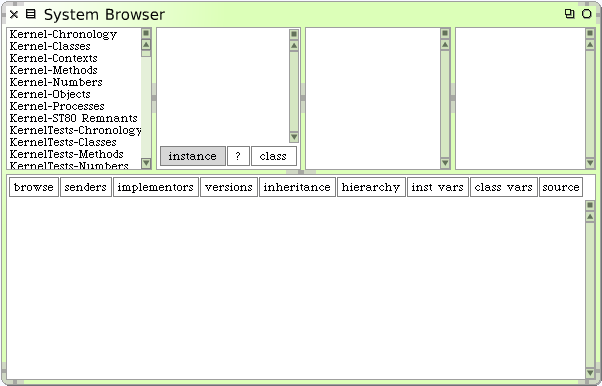
\includegraphics[width=\textwidth]{SystemBrowser0} }
	 {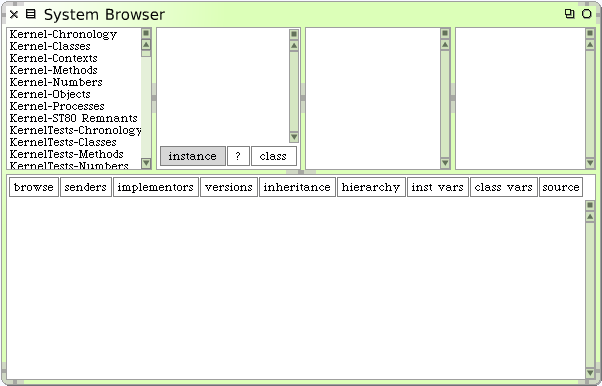
\includegraphics[scale=.7]{SystemBrowser0} }
   \caption{Le navigateur de classes: System Browser.}
   \label{fig:SystemBrowser0}
\end{figure}

Les quatre petits panneaux en haut du Browser repr\'esentent la vue
hi\'erarchique des m\'ethodes dans le syst\`eme de la m\^eme
mani\`ere que le \textit{File Viewer} de \ind{NeXTstep} et le
\textit{Finder} de Mac OS X fournissent une vue en colonnes 
des fichiers du disque.

Le premier panneau de gauche liste les \emph{cat\'egories} de classes;
s\'electionnez-en une (disons \scat{Kernel-Objects}) et alors le
panneau imm\'ediatemment \`a droite affichera toutes les classes incluses
dans cette cat\'egorie.
\on{I adopted the spelling of NeXTstep recommended by wikipedia}

\begin{figure}[htbp]
   \centering
   \ifluluelse
	   {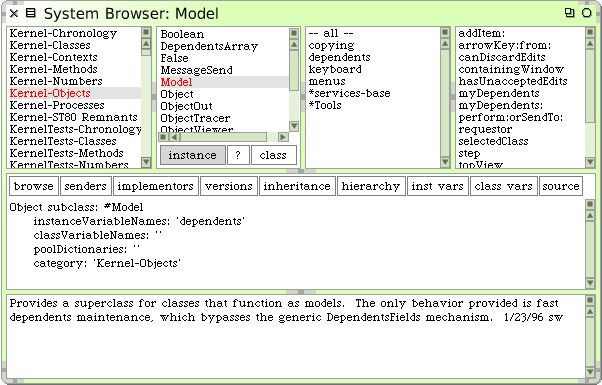
\includegraphics[width=\textwidth]{SystemBrowser1} }
	   {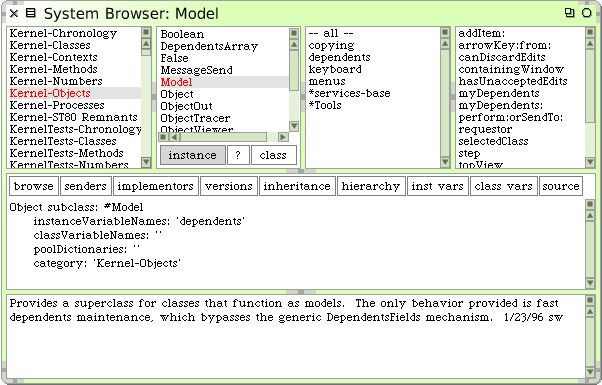
\includegraphics[scale=.7]{SystemBrowser1} }
   \caption{Le System Browser avec la classe \ct{Model} s\'electionn\'ee.
   \label{fig:SystemBrowserModel}}
\end{figure}

De m\^eme, si vous s\'electionnez une des classes de ce second panneau,
disons, \menu{Model} (voir  \figref{SystemBrowserModel}), le troisi\`eme
panneau vous affichera tous les \emph{protocoles} d\'efinis pour cette
classe ainsi qu'un protocole virtuel \prot{-{}-all-{}-} (d\'esignant l'ensemble des cat\'egories). Ce dernier est s\'electionn\'e par d\'efaut. 
Les protocoles sont une fa\c{c}on de cat\'egoriser les m\'ethodes;
ils rendent la recherche des m\'ethodes plus facile et d\'etaillent
le comportement d'une classe en le d\'ecoupant en petites divisions 
coh\'erentes.
% they make it easier to find and think about the behaviour of a class by breaking it up into smaller, conceptually coherent pieces.  
Le quatri\`eme panneau montre les noms de toutes les m\'ethodes d\'efinies dans le protocole s\'electionn\'e.
Si vous s\'electionnez enfin un nom de m\'ethode, le code source de la 
m\'ethode correspondante appara\^{\i}t dans le grand panneau inf\'erieur
du navigateur. L\`a, vous pouvez voir, \'editer et sauvegarder la version \'edit\'ee.
Si vous s\'electionnez la classe
\menu{Model}, le protocole \protind{dependents} et la m\'ethode \menu{myDependents}, le navigateur devrait ressembler \`a \figref{SystemBrowserMyDependents}.
\protindex{all}
\cmindex{Model}{myDependents}

\begin{figure}[htbp]
   \centering
   \ifluluelse
	   {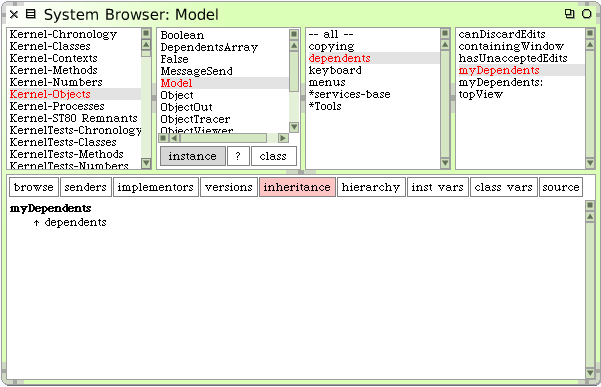
\includegraphics[width=\textwidth]{SystemBrowserMyDependents}}
	   {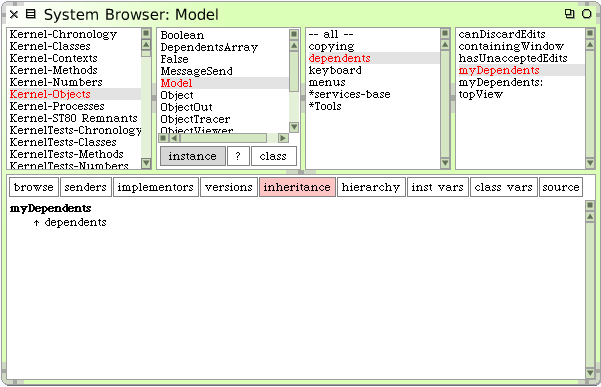
\includegraphics[scale=.7]{SystemBrowserMyDependents}}
   \caption{Le System Browser affichant la m\'ethode \ct{myDependents} de la classe \ct{Model}.
   \label{fig:SystemBrowserMyDependents}}
\end{figure}

Contrairement aux r\'epertoires du \emph{Finder} de Mac OS X, les quatre panneaux sup\'erieurs ne sont aucunement \'egaux.
L\`a o\`u les classes et les m\'ethodes font partie du langage \st,
les cat\'egories syst\`eme et les protocoles de message ne sont
que des convenances introduites par le navigateur pour limiter la quantit\'e d'information que chaque panneau pourrait pr\'esenter.
Par exemple, s'il n'y avait pas de protocoles, le navigateur devrait afficher
la liste de toutes les m\'ethodes dans la classe choisie; pour la plupart des classes, cette liste sera trop importante pour \^etre parcourue ais\'ement.
\index{Mac OS X Finder}

De ce fait, la fa\c{c}on dont vous cr\'eez une nouvelle cat\'egorie ou
un nouveau protocole est diff\'erent de la mani\`ere avec laquelle
vous cr\'eez une nouvelle classe ou une nouvelle m\'ethode. 
Pour cr\'eer une nouvelle cat\'egorie, s\'electionnez 
 \menu{new category} via le menu contextuel acc\'ed\'e avec le bouton \ind{jaune}
% martial: yellow button | bouton central
 dans le panneau des cat\'egories; pour cr\'eer un nouveau protocole, 
s\'electionnez \menu{new protocol} via le menu acc\'ed\'e avec
le m\^eme bouton dans le panneau des protocoles.
Entrez le nom de la nouvelle entit\'e (cat\'egorie ou protocole) dans
la zone de saisie, et voil\`a! 
% dialog
Une cat\'egorie ou un protocole, \c{c}a n'est qu'un nom et son contenu.
\index{cat\'egorie!cr\'eation}

\begin{figure}[htbp]
   \centering
   \ifluluelse
	   {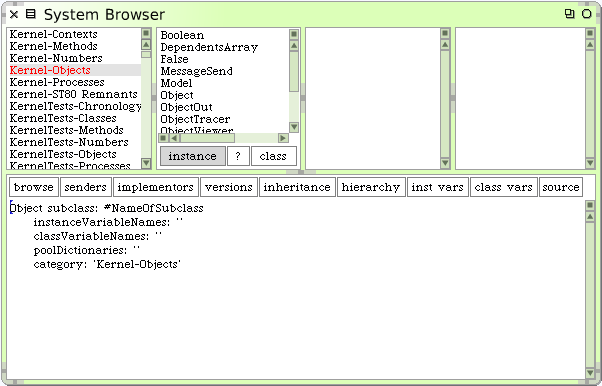
\includegraphics[width=\textwidth]{SystemBrowserClassCreation}}
	   {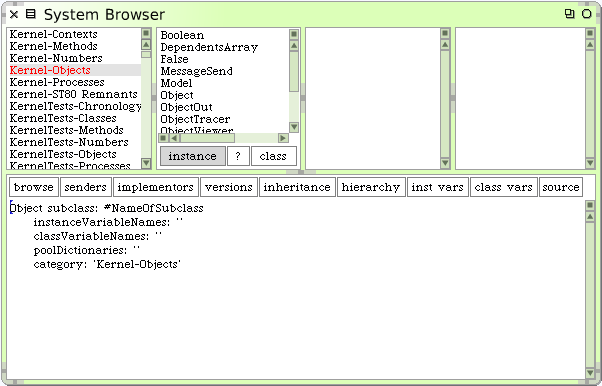
\includegraphics[scale=.7]{SystemBrowserClassCreation}}
   \caption{Le System Browser montrant le patron de cr\'eation de classe.
   \label{fig:SystemBrowserClassCreation}}
\end{figure}

\`A l'oppos\'e, cr\'eer une classe ou une m\'ethode nouvelle n\'ecessite 
l'\'ecriture de code \st.
Si vous d\'es\'electionnez la classe actuellement s\'electionn\'ee de mani\`ere \`a ce qu'aucune classe ne soit s\'electionn\'ee, le panneau principal 
affichera un patron de cr\'eation de classe
(voir \figref{SystemBrowserClassCreation}).
Vous cr\'eez une nouvelle classe en \'editant ce patron ou \emph{template}. Pour se faire, remplacez \ct{Object} par le nom de la classe existante
que vous voulez d\'eriver, puis remplacez \ct{NameOfSubclass} par le nom
que vous avez choisi pour votre nouvelle classe (sous-classe de la premi\`ere) et enfin, remplissez la liste des noms de variables d'instance si vous en connaissez.  
La cat\'egorie pour la nouvelle classe est par d\'efaut la cat\'egorie actuellement s\'electionn\'ee mais vous pouvez changer celle-ci aussi si vous le d\'esirez.
Si vous avez d\'ej\`a la classe \`a d\'eriver s\'electionn\'ee dans 
le Browser, vous pouvez obtenir le m\^eme patron avec une initialisation
quelque peu diff\'erente en utilisant le menu du bouton jaune
% yellow
dans le panneau des classes et en s\'electionnant 
 \menu{more \ldots \go subclass template}.
Vous pouvez aussi \'editer simplement la d\'efinition de la classe existante en changeant le nom de la classe en quelque chose d'autre.
Dans tous les cas, \`a chaque fois que vous acceptez la nouvelle d\'efinition, la nouvelle classe 
(celle dont le nom est pr\'ec\'ed\'e par \ct{#}) est cr\'e\'ee (ainsi que sa m\'eta-classe associ\'ee).  
Cr\'eer une classe cr\'ee aussi une variable globale r\'ef\'eren\c{c}ant
la classe. En fait, l'existence de celle-ci vous permet de vous 
r\'ef\'erer \`a toutes les classes existantes en utilisant leur nom.
\index{classe!cr\'eation}
\index{system browser!d\'efinition d'une classe}
\index{navigateur de classe!d\'efinition d'une classe}

Voyez-vous pourquoi le nom d'une nouvelle classe doit appara\^{\i}tre
comme un \clsind{Symbol} (\ie pr\'efix\'e avec \ct{#}) dans le
patron de cr\'eation de classe, mais qu'apr\`es la cr\'eation
de classe, le code peut s'y r\'ef\'erer en utilisant
son nom comme identifiant (\ie sans le \ct{#})?

Le processus de cr\'eation d'une nouvelle m\'ethode
est similaire. Premi\`erement s\'electionnez la classe dans laquelle vous
voulez que la m\'ethode apparaisse, puis s\'electionnez un protocole.
Le navigateur affichera un patron de cr\'eation de m\'ethode que
vous pouvez remplir et \'editer, comme montr\'e par
\figref{SystemBrowserMethodTemplate}.
\index{m\'ethode!cr\'eation}
\index{System Browser!d\'efinition d'une m\'ethode}
\index{navigateur de classe!d\'efinition d'une m\'ethode}


\begin{figure}[htbp]
   \centering
   \ifluluelse
	   {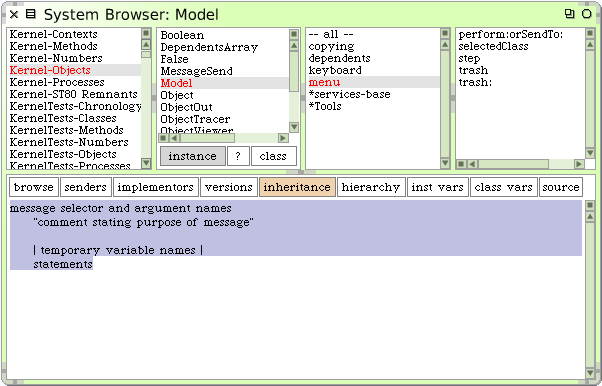
\includegraphics [width=\textwidth]{SystemBrowserMethodTemplate}}
	   {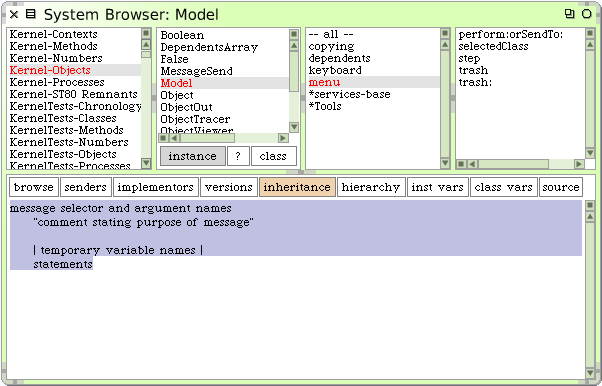
\includegraphics[scale=.7]{SystemBrowserMethodTemplate}}
   \caption{Le System Browser montrant le patron de cr\'eation de m\'ethode.
   \label{fig:SystemBrowserMethodTemplate}}
\end{figure}

%---------------------------------------------------------
\subsection{La barre de boutons}
\label{sec:ButtonBar}

Le System Browser fournit plusieurs outils pour l'exploration et 
l'analyse de code. 
% rene rewording
L'acc\`es le plus courant \`a ces outils s'effectue via la 
% Ces outils sont acc\'ed\'es le plus commun\'ement via la 
\subind{System Browser}{barre de boutons} horizontale au milieu
de la fen\^etre du navigateur. Les boutons sont lab\'elis\'es 
\button{browse}, \button{senders}, \button{implementors}\ldots{}\ %
\figref{SystemBrowserMethodTemplate} montre la liste compl\`ete.

\subsubsection{Naviguer dans le code}
\label{sec:browsing}

Le bouton \button{browse} ouvre une nouvelle fen\^etre de navigateur sur
la classe ou la m\'ethode s\'electionn\'ee. Il est souvent utile d'avoir
plusieurs navigateurs ouverts au m\^eme moment. Quand vous
\'ecrivez du code, vous aurez presque toujours besoin d'au moins deux
fen\^etres: une pour la m\'ethode que vous \'editez et une pour naviguer
dans le reste du syst\`eme pour y voir ce dont vous aurez besoin pour la
m\'ethode \'edit\'ee dans la premi\`ere. Vous pouvez tout aussi bien
ouvrir un navigateur sur une classe en s\'electionnant son nom et en utilisant le raccourci-clavier \short{b} \ind{raccourci-clavier}.
\index{System Browser!bouton browse}
\index{raccourci-clavier!browse it}

\dothis{Essayez ceci: dans un espace de travail ou Workspace, saisissez le nom d'une classe (par exemple, \ct{ScaleMorph}), s\'electionnez-le et pressez \short{b}. Cette astuce est souvent utile; elle marche depuis n'importe quelle fen\^etre de texte.}

\subsubsection{Senders et implementors d'un message}
\label{sec:sendersImplementors}

\index{System Browser!bouton senders}
Le bouton \button{senders} vous renvoie \`a une liste de toutes les m\'ethodes
pouvant utitliser la m\'ethode s\'electionn\'ee. En prenant le navigateur ouvert sur \ct{ScaleMorph}, cliquez sur la m\'ethode \mthind{ScaleMorph}{checkExtent:} dans le panneau des m\'ethodes dans le coin sup\'erieur droit du navigateur;
le corps
 de \ct{checkExtent:} affich\'e dans sa partie inf\'erieure.
Si vous appuyez maintenant sur le bouton \button{senders}, 
un menu appara\^{\i}tra avec \ct{checkExtent:} comme premier \'element de
la pile, suivi de tous les messages que \ct{checkExtent:} envoie (voir \figref{SendersOfCheckEvent}). 
S\'electionner un message dans ce menu ouvrira un navigateur avec la liste de toutes les m\'ethodes dans l'image qui envoie le message choisi.

\begin{figure}[htbp]
	\begin{center}
   \ifluluelse
		{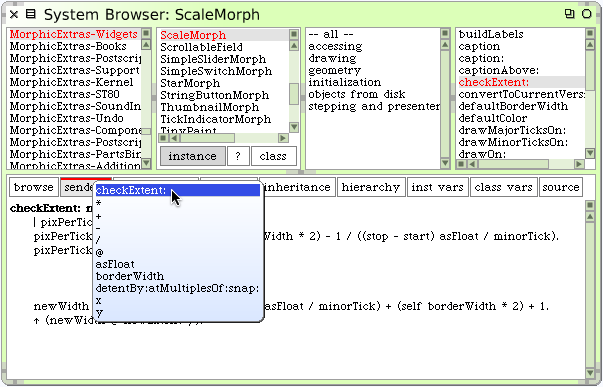
\includegraphics[width=\textwidth]{SendersOfCheckEvent}}
		{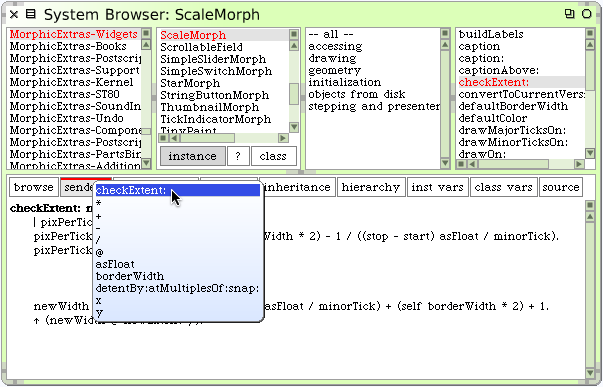
\includegraphics[scale=0.7]{SendersOfCheckEvent}}
	\end{center}
	\caption{Un navigateur de classes ouvert sur la classe \ct{ScaleMorph}. Notez la barre horizontale de boutons en son centre; nous appuyons ici sur le bouton \button{senders}.
	\label{fig:SendersOfCheckEvent}}
\end{figure}

\index{System Browser!bouton implementors}
Le bouton \button{implementors} fonctionne de la m\^eme mani\`ere mais,
au lieu de renvoyer une liste de senders d'un message (ou m\'ethodes-envoyeuses), il sort toutes les
classes qui impl\'ementent une m\'ethode avec le m\^eme s\'electeur.
Pour le voir, s\'electionnez \lct{drawOn:} dans le panneau des m\'ethodes
puis affichez le navigateur ``implementors of drawOn:'', 
soit en utilisant le bouton \button{implementors}, soit via le bouton 
\ind{jaune}, soit encore en tapant simplement \short{m} (pour {i\textbf{m}ple\textbf{m}entors}) avec la m\'ethode \menu{drawOn:} s\'electionn\'ee dans le panneau des m\'ethodes. 
Vous devriez avoir une fen\^etre \`a ascenseur montrant une liste des 96
classes impl\'ementant une m\'ethode \ct{drawOn:}.
Il n'y a rien de surprenant \`a ce qu'autant de classes impl\'ementent cette
m\'ethode: \ct{drawOn:} est le message compris par tout objet apte \`a se
dessiner lui-m\^eme sur l'\'ecran.
Essayez de naviguer dans la liste des senders du message \ct{drawOn:}; nous nous trouvons face \`a 63 m\'ethodes \'emettrices. Vous pouvez aussi ouvrir
un navigateur d'implementors chaque fois que vous s\'electionnez un message
(en incluant les arguments s'il s'agit d'un message \`a mots-cl\'es) puis
que vous appuyez sur \short{m}.

%The \menu{senders} button lists \emph{all} the methods that send the chosen message: not all of these message sends will necessarily be able to cause the execution of any particular method with the same selector.
%Indeed, much of the power of object-oriented programming comes from the fact that every message send is potentially \emph{polymorphic}, that is, it can work equally well on objects of any class.  Sometimes it is easy to figure out which method will be executed as result of a particular message send, and sometimes it is impossible; the senders and implementors tools don't try.
% APB: commented-out because the same thought is expressed below.

Si vous regardez l'envoi de \ct{drawOn:} dans \ct{AtomMorph>>>drawOn:}, vous
verrez que c'est un \subind{super}{envoi} de super. Ainsi nous
savons que la m\'ethode ex\'ecut\'ee sera dans la super-classe de \ct{AtomMorph}. Quelle est cette classe? Cliquez sur le bouton \button{hierarchy} (pour hi\'erarchie) et vous saurez qu'il s'agit de \ct{EllipseMorph}.
\index{System Browser!bouton hierarchy}

\begin{figure}[htbp]
	\begin{center}
   \ifluluelse
		{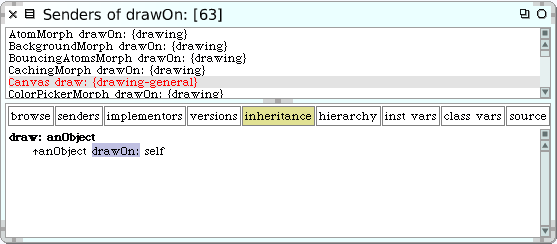
\includegraphics[width=\textwidth]{CanvasDraw}}
		{\includegraphics[scale=0.7]{CanvasDraw}}
	\end{center}
	\caption{Le navigateur Senders Browser montrant que la m\'ethode \ct{Canvas>>>>draw} envoie le message \ct{drawOn:} \`a son argument.	\label{fig:CanvasDraw}}
\end{figure}

Maintenant observons le cinqui\`eme \emph{sender} de la liste, \ct{Canvas>>>>draw}, comme le montre \figref{CanvasDraw}.
Vous pouvez voir que cette m\'ethode envoie \ct{drawOn:} \`a n'importe quel objet pass\'e en argument; ce peut \^etre une instance de n'importe quelle classe.
L'analyse du flux de donn\'ees peut nous aider \`a mettre la main sur la classe du receveur de certains messages, mais de mani\`ere g\'en\'erale, il n'a pas de moyen simple pour que le navigateur sache quelle m\'ethode sera ex\'ecut\'ee \`a l'envoi d'un message.
%Dataflow analysis can help figure out the class of the receiver of some messages, but in general, there is no simple way for the browser to know which message-sends might cause which methods to be executed.

C'est pourquoi, le navigateur de ``senders'' (\ie le Browser des m\'ethodes \'emettrices) nous montre exactement ce que son nom sugg\'ere: tous les envois d'un message ayant le s\'electeur choisi.
N'importe comment, le bouton \button{senders} devient grandement indispensable
quand vous avez besoin de comprendre le \emph{r\^ole} d'une m\'ethode: il vous permet de naviguer rapidement \`a travers les exemples d'usage.
%The \button{senders} button is nevertheless extremely useful when you need to understand how you can \emph{use} a method: it lets you navigate quickly through example uses.  
Puisque toutes les m\'ethodes avec un m\^eme s\'electeur devraient \^etre utilis\'ee de la m\^eme mani\`ere, toutes les utilisations d'un message donn\'e devrait \^etre semblable.
\index{System Browser!bouton senders}

\subsubsection{Les versions d'une m\'ethode}
\label{sec:versions}

Quand vous sauvegardez une nouvelle \subind{m\'ethode}{version} d'une m\'ethode,
l'ancienne version n'est pas perdue. \sq garde toutes les versions pass\'ees et vous permet de comparer les diff\'erentes versions entre elles et de revenir (en anglais, ``revert'') \`a une ancienne version.
\begin{figure}[btp]
   \centering
   \ifluluelse
	   {\includegraphics[width=\textwidth]{VersionsOfMouseUp} }
	   {\includegraphics[scale=0.7]{VersionsOfMouseUp} }
   \caption{Le \ind{Versions Browser} montre plusieurs versions de la m\'ethode \ct{SBECell>>>mouseUp:}.}
   \label{fig:mouseUpVersions}
\end{figure}
Le bouton \button{versions} donne acc\`es aux modifications successives
effectu\'ees sur la m\'ethode s\'electionn\'ee.
Dans \figref{mouseUpVersions} nous pouvons voir les versions de la m\'ethode \ct{mouseUp:} qu'un des auteurs a cr\'e\'ee lors de l'\'ecriture du jeu de \emph{Quinto} d\'ecrit dans \charef{firstApp}.
\index{System Browser!bouton versions}

Le panneau sup\'erieur affiche une ligne pour chaque version de la m\'ethode
incluant les initiales du programmeur qui l'a \'ecrite, la date et l'heure de
sauvegarde, les noms de la classe et de la m\'ethode et le protocole dans 
lequel elle est d\'efinie.
La version courante (active) est au sommet de la liste; quelque soit la version
s\'electionn\'ee affich\'ee dans le panneau inf\'erieur.
Si le bouton (checkbox) \menu{diffs} est s\'electionn\'e, 
comme c'est le cas dans \figref{mouseUpVersions}, 
les diff\'erences entre la version s\'electionn\'ee et celle qui la pr\'ec\`ede
imm\'ediatemment sont affich\'ees.
Les boutons offrent aussi l'affichage des diff\'erences entre la m\'ethode s\'electionn\'ee et la version courante et la possibilit\'e de revenir \`a la version choisie.  
Le bouton \menu{prettyDiffs} est utile s'il y a eu changement dans la mise en
pages: il affiche en mode \emph{pretty-print} (affichage \'el\'egant) 
\`a la fois les versions ant\'erieures et choisies de fa\c{c}on \`a
ce que les diff\'erences li\'ees au formatage ne soient pas prises en compte.

Le \ind{Versions Browser} existe pour que vous ne vous inqui\'etez jamais
de la pr\'eservation de code que vous pensiez ne plus avoir besoin: effacez-le simplement. Si vous vous rendez compte que vous en avez \emph{vraiment} besoin, 
vous pouvez toujours revenir \`a l'ancienne version ou copier le morceau de 
code utile de la version ant\'erieure pour le coller dans une autre m\'ethode.

Ayez pour habitude d'utiliser les versions; ``commenter'' le code qui n'est plus utile n'est pas une bonne pratique car \c{c}a rend le code courant plus
difficile \`a lire. Les Smalltalkiens~\footnote{En anglais, nous les appelons
 \emph{Smalltalkers}.} accorde une extr\^eme importance \`a la lisibilit\'e du code.

\hint{Qu'en est-il du cas 
o\`u vous d\'ecidez de revenir \`a une m\'ethode que vous
avez enti\`erement effac\'ee?  
Vous pouvez trouver l'effacement dans un \changeset
dans lequel vous pouvez demander \`a visiter les versions via le menu du
\ind{bouton jaune}. Le navigateur de \changeset est d\'ecrit dans
\secref{env:changeSet}}

\subsubsection{Les surcharges de m\'ethodes}
\label{sec:overriding}

Le bouton \button{inheritance} ouvre un navigateur sp\'ecialis\'e affichant
toutes les m\'ethodes surcharg\'ees par la m\'ethode affich\'ee.
Pour voir son fonctionnement, affichez la m\'ethode
\cmind{ScaleMorph}{defaultColor} et cliquez sur \button{inheritance}.
La d\'efinition de cette m\'ethode surcharge 
\mbox{\cmind{RectangleMorph}{defaultColor},} elle-m\^eme surchargeant
\cmind{Morph}{defaultColor}, comme montr\'e dans \figref{inheritanceOverriding}.
La couleur du bouton \button{inheritance} d\'epend 
de comment s'op\`ere la \subind{m\'ethode}{surcharge}. 
Les couleurs sont expliqu\'ees dans le ballon d'aide ou \emph{help balloon}:
\index{System Browser!bouton inheritance}

\newcommand{\colourTag}[1]{\item[{\mdseries \itshape #1}]}

\begin{description}[noitemsep, leftmargin=*, labelindent=6em, labelwidth=4em, labelsep=*]
	\colourTag{rose:} la m\'ethode affich\'ee surcharge une autre m\'ethode mais ne l'utilise pas;
	\colourTag{vert:} la m\'ethode affich\'ee surcharge une autre m\'ethode et l'utilise via \super;
	\colourTag{or:} la m\'ethode affich\'ee est elle-m\^eme surchag\'ee dans une sous-classe;
	\colourTag{saumon:} la m\'ethode affich\'ee surcharge une autre m\'ethode et est elle-m\^eme surcharg\'ee;
	%\colourTag{violet:} 
	\colourTag{mauve:} la m\'ethode affich\'ee surcharge, est surcharg\'ee et \'emet un envoi sur \ct{super}.
\end{description}

\begin{figure}[tbp]
	\begin{center}
   \ifluluelse
		{\includegraphics[width=\textwidth]{inheritanceOverriding}}
		{\includegraphics[scale=0.7]{inheritanceOverriding}}
	\end{center}
	\caption{\ct{ScaleMorph>>>defaultColor} et les m\'ethodes qu'il surcharge dans l'ordre hi\'erarchique d'h\'eritage. 
	Le bouton \button{inheritance} est de couleur or parce que la m\'ethode affich\'ee est surcharg\'ee dans une sous-classe.}
	\label{fig:inheritanceOverriding}
\end{figure}

Notez qu'il y a deux versions de ce navigateur. Si vous utilisez la version du
System Browser bas\'ee sur la librairie applicative (ou framework) \ind{OmniBrowser}, le bouton \button{inheritance} ne change pas de couleur et Inheritance Browser a une apparence diff\'erente.  
Il propose aussi plus d'informations en n'affichant pas seulement les m\'ethodes de la cha\^{\i}ne d'h\'eritage mais aussi les m\'ethodes apparent\'ees (ou fr\`eres~\footnote{En anglais, siblings.}) comme le montre \figref{OBinheritanceBrowser}.

\begin{figure}[btp]
	\begin{center}
   \ifluluelse
		{\includegraphics[width=\textwidth]{OBInheritanceOverriding}}
		{\includegraphics[scale=0.7]{OBInheritanceOverriding}}
	\end{center}
	\caption{\ct{ScaleMorph>>>defaultColor} et les m\'ethodes qu'il surcharge, comme nous pouvons le voir avec le nouveau Inheritance Browser bas\'e sur OmniBrowser. Les m\'ethodes apparent\'ees des m\'ethodes s\'electionn\'ees sont montr\'ees dans des listes.}
	\label{fig:OBinheritanceBrowser}
\end{figure}


\subsubsection{Le navigateur hi\'erarchique}
\label{sec:hierarchy}

Le bouton \button{hierarchy} ouvre un navigateur hi\'erarchique ou
\ind{Hierarchy Browser} sur la classe actuelle; ce navigateur peut aussi \^etre ouvert en utilisant \menu{browse hierarchy} dans le menu du
panneau de classe.
Le Hierarchy Browser se pr\'esente comme le System Browser \`a cette exception
pr\`es qu'il affiche une simple liste de classes indent\'ees pour repr\'esenter
l'h\'eritage l\`a o\`u le navigateur de classes classique affiche les cat\'egories et les classes dans chaque cat\'egorie.
La cat\'egorie de la classe s\'electionn\'ee appara\^{\i}t en annotation
dans un panneau sup\'erieur horizontal.
Le navigateur hi\'erarchique est destin\'e \`a faciliter la navigation au travers de la hi\'erarchie d'h\'eritage mais, au lieu de montrer toutes
les classes du syst\`eme, il affiche seulement les super-classes ou
sous-classes de la classe initiale. 
Dans \figref{hierarchyBrowser}, le navigateur hi\'erarchique nous
informe que \clsind{RectangleMorph} est la super-classe directe de 
\clsind{ScaleMorph}.
\index{System Browser!bouton hierarchy}

\begin{figure}[btp]
	\begin{center}
	\ifluluelse
		{\includegraphics[width=\textwidth]{hierarchyBrowser}}
		{\includegraphics[scale=0.7]{hierarchyBrowser}}
	\end{center}
	\caption{Un Hierarchy Browser ouvert sur \ct{ScaleMorph}.}
	\label{fig:hierarchyBrowser}
\end{figure}

\subsubsection{Trouver les r\'ef\'erences aux variables}
\label{sec:variables}

\index{System Browser!bouton inst vars}
\index{System Browser!bouton class vars}
Les boutons \button{inst vars} et \button{class vars} vous aident \`a savoir
dans quelles m\'ethodes sont utilis\'ees respectivement les variables d'instance
et les variables de classe; cette information est aussi disponible depuis 
\menu{inst var refs} et \menu{class var refs} du menu contextuel accessible via le 
\ind{bouton jaune} dans le panneau de la classe.
Le menu permet aussi d'afficher le jeu 
%subset 
des r\'ef\'erences aux variables d'instance qui affecte la variable choisie
par \menu{inst var defs}.
Une fois que vous avez cliqu\'e sur le bouton ou que vous avez choisi une
des propositions de menu, un menu flottant s'affichera, vous invitant ainsi
\`a s\'electionner une variable parmi toutes les variables d\'efinies et
h\'erit\'ees dans la classe courante.
La liste suit l'ordre d'h\'eritage; il peut d'ailleurs \^etre utile d'afficher
cette liste \`a chaque fois vous avez besoin de vous rem\'emorer le nom d'une
variable d'instance. Si vous cliquer en dehors de la liste, cette derni\`ere
dispara\^{\i}tra sans avoir affich\'e le navigateur de variable.

Signalons que nous pouvons acc\'eder \`a \menu{class vars},
gr\^ace au menu de panneau de classes accessible par le bouton jaune
de la souris, 
ouvrant donc un inspecteur affichant les variables de classe 
de la classe actuelle ainsi que \emph{leurs valeurs};
ou encore \`a
\menu{class refs (N)} affichant une liste de toutes les m\'ethodes
r\'ef\'eren\c{c}ant directement cette m\^eme classe.

\subsubsection{Le panneau source}
\label{sec:sources}

\index{System Browser!bouton source}
Le bouton \button{source} affiche un menu que nous pourrions appeler
%``what to show'' menu, 
``ce qui est \`a voir''; il nous permet de choisir ce que le navigateur
affiche dans le panneau inf\'erieur ou panneau source.
Parmi les propositions, nous avons l'affichage du code \menu{source}, 
du code source en mode \menu{prettyPrint} (affichage \'el\'egant), 
du code compil\'e ou \menu{byteCodes} ou encore du code source
d\'ecompil\'e depuis les \emph{bytes codes} via \menu{decompile}.
Le label du bouton change pour afficher le mode choisi. Il y a d'autres
options; si vous promenez la souris sur ces options, vous verrez
appara\^{\i}tre un ballon d'aide (ou \emph{help balloon}). Essayez-en
quelques-uns. 
\index{m\'ethode!pretty-print}
\index{m\'ethode!decompile}
\index{m\'ethode!byte code}

Remarquez que le choix de \menu{prettyPrint} dans ce menu n'est \emph{absolument pas} le m\^eme que le travail en mode \emph{pretty-print} d'une m\'ethode
avant sa sauvegarde.
Le menu contr\^ole seulement l'affichage du navigateur et n'a aucun effet sur
le code enregistr\'e dans le syst\`eme.
Vous pouvez le v\'erifier en ouvrant deux navigateurs et en s\'electionnant
\menu{prettyPrint} pour l'un et \menu{source} pour l'autre.
Pointer les deux navigateurs sur la m\^eme m\'ethode et en choisissant
\menu{byteCodes} dans l'un et \menu{decompile} dans l'autre est vraiment
une bonne mani\`ere d'en apprendre plus sur le jeu d'instructions cod\'ees
(dit aussi \emph{byte-cod\'ees}) de la machine virtuelle \sq.

\subsubsection{La refactorisation}
% ou r\'eusinage

\index{System Browser!bouton refactor}

Avez-vous not\'e la petit bouton \button{R} au bout de la barre de 
boutons?~\footnote{Ceci dit, vous n'observerez pas ce bouton sans
que les paquetages AST et RefactoringBrowser ne soit install\'e. Ces
paquetages sont accessibles sur SqueakSource ou dans une image \emph{Squeak-dev}.}
Ce bouton tr\`es discret donne acc\`es \`a une des techniques
les plus importantes et les plus puissantes de l'environnement de
Smalltalk.
En cliquant sur \button{R}, vous obtenez une hi\'erarchie de menus
pour refactoriser (\cad r\'eusiner~\footnote{\emph{Refactoring} en anglais.}) votre code.
Il existe d'autres fa\c{c}ons d'obtenir l'outil de refactorisation. Par
exemple, via le menu accessible par le \ind{bouton jaune} dans les
panneaux de classes, de m\'ethodes et de code.
\`A l'origine, cette fonction \'etait disponible uniquement
par un navigateur sp\'ecifique nomm\'e Refactoring Browser, mais
elle peut d\'esormais \^etre accessible depuis n'importe quel navigateur.

%---------------------------------------------------------
\subsection{Les menus du navigateur}

De nombreuses fonctions compl\'ementaires sont disponibles dans les menus du
System Browser accessibles par le bouton jaune. Ces menus sont contextuels, 
autrement dit, chaque panneau a son propre menu.
M\^eme si les \'elements du menu ont le m\^eme nom, leur \emph{signification}
d\'epend du contexte. Par exemple, le panneau de cat\'egories, le
panneau de classes, le panneau de protocoles et enfin, celui des messages
ont tous \menu{file out} dans leurs menus respectifs. Cependant, chaque 
\menu{file out} fait une chose diff\'erente: dans le panneau des cat\'egories,
il enregistre enti\`erement dans un fichier la cat\'egorie s\'electionn\'ee; dans le celui des classes, des protocoles ou des messages, il exporte respectivement la classe enti\`ere, le protocole entier ou la m\'ethode affich\'ee.
Bien qu'apparemment \'evident, ce peut \^etre une source de confusion pour
les d\'ebutants. 
\index{fichier!filing in}
\index{fichier!importation}
\index{fichier!filing out}
\index{fichier!exportation}

L'option probablement la plus utile du menu est \menu{find class\ldots (f)} 
dans le panneau de cat\'egories. 
Elle permet de trouver une classe.  
% ajout
Bien que les cat\'egories soient utiles pour arranger le code que nous 
sommes en train de d\'evelopper, la plupart d'entre nous ne connaissent pas
la cat\'egorisation de tout le syst\`eme, et c'est beaucoup plus rapide
en tapant \short{f} suivi par les premiers caract\`eres du nom d'une 
classe que de deviner dans quelle cat\'egorie elle peut bien \^etre.
\menu{recent classes\ldots (r)} vous aide aussi \`a retrouver rapidement
une classe parmi celles que vous avez visit\'ees r\'ecemment, m\^eme si vous
avez oubli\'e son nom.
\index{classe!trouver}
\index{classe!r\'ecente}

Dans le panneau de classes, le menu propose \menu{find method} (pour ``trouver
une m\'ethode'') et
\menu{find method wildcard\ldots} qui s'av\`erent utiles si vous souhaitez
naviguer dans une m\'ethode particuli\`ere. Cependant, 
\`a moins que la liste des m\'ethodes soient tr\`es longues, il est souvent
plus efficace de naviguer dans le protocole \prot{-{}-all-{}-} 
(qui d'ailleurs est le choix par d\'efaut), placer la souris dans le
panneau des m\'ethodes et taper la premi\`ere lettre du nom de la m\'ethode
que vous cherchez.
Ceci va faire glisser l'ascenseur du panneau jusqu'\`a ce que la m\'ethode souhait\'ee soit visible.
\index{m\'ethode!trouver}
\protindex{all}

\dothis{Essayez les deux techniques de navigation pour \cmind{OrderedCollection}{removeAt:}}

Il y a beaucoup d'autres options dans les menus.  Passer quelques
minutes \`a tester les possibilit\'es du navigateur est v\'eritablement payant.  

\dothis{Comparez le r\'esultat de \menu{Browse Protocol}, \menu{Browse Hierarchy},  et \menu{Show Hierarchy} dans le menu contextuel du panneau de classes.}

%---------------------------------------------------------
\subsection{Les autres navigateurs de classes}
\label{sec:otherBrowsers}

Au d\'ebut de cette section nous avons mentionn\'e un autre navigateur:
le \emphind{Package Pane Browser}. 
Il peut \^etre ouvert via le menu World: \menu{World \go open\ldots \go package pane browser}.
Il se pr\'esente comme le navigateur de classes sauf qu'il conna\^{\i}t
les conventions de nommage des cat\'egories-syst\`eme.
Vous aurez not\'e que les noms des cat\'egories sont d\'ecompos\'es en deux
parties.
Par exemple, la classe \ct{ScaleMorph} appartient \`a la cat\'egorie
\scat{Morphic-Widgets}.
\label{sec:package-names}
Le Package Browser suppose que la partie pr\'ec\'edant le trait d'union
(soit \ct{Morphic}) est le nom du ``paquetage'' ou ``package''. 
Il ajoute une cinqui\`eme
colonne permettant de naviguer dans les cat\'egories de chaque paquetage particulier. Cependant, si vous ne choisissez aucun paquetage, toutes les cat\'egories
seront disponibles 
(avec leur nom entier)
% ajout
comme avec un navigateur ordinaire \`a quatre panneaux.

Malheureusement, le sens donn\'e au terme \ind{paquetage} a chang\'e depuis
le d\'eveloppement du Package Pane Browser. ``Package'' a aujourd'hui
une d\'efinition plus pr\'ecise en accord avec l'outil de gestion
de paquetages \emph{Monticello}. Nous aborderons cet outil dans la
prochaine section.  Il n'y a pour l'instant aucun outil pour naviguer
dans les paquetages tels qu'ils sont arrang\'es dans \ind{Monticello}, cependant
une telle application est en cours de d\'eveloppement.
\seeindex{package}{paquetage}

La communaut\'e \sq est en train de d\'evelopper toute une famille de nouveaux
navigateurs reposant sur une nouvelle librairie tr\`es adaptable nomm\'ee
\emphind{OmniBrowser}.  L'impl\'ementation de OmniBrowser vaut d'\^etre 
\'etudi\'ee au moins comme un bon exemple de \emph{conception} orient\'ee
objet. \ab{and I'd like to add a chapter on it somewhere, perhaps starting with parts of the excellent document written by Niklaus Haldimann on the classbox browser}
Du reste, la plupart des outils bas\'es sur OmniBrowser ressemblent beaucoup
\`a ceux que nous avons d\'ecrits.
L'am\'elioration principale que vous remarquerez dans l'Omni System Browser 
est l'ajout de \emph{protocoles virtuels} ou \emph{virtual protocols}.
%\lr{"Virtual Protocols" are a non-default extension to OB (p. 140)}
Aux protocoles traditionnellement d\'efinis par le programmeur s'ajoutent
un certain nombre de protocoles virtuels d\'efinis pour chaque classe 
par des syst\`emes de r\`egles. 
% definitional rules
Par exemple, le protocole \prot{-{}-supersend-{}-} inclus toutes
les m\'ethodes qui envoie \super, alors que le protocole
 \prot{-{}-required-{}-} liste tous les messages qui sont \'emis
par les m\'ethodes dans la classe courante ou ses super-classes 
mais qui n'y sont pas d\'efinies.
\protindex{supersend}
\protindex{required}

\on{Is this related to abstract methods or not?  It is not clear.}

\ab{You are right, it's not clear.  The definition of abstract method that we have given is a method that has \ct{self subclassResponsibility} as a body.
By this definition, the two things are different.  I happen to think that the definition that we used for required method is better, and should be adopted for abstract method, \ie an abstract method is one that is either required, or has a marker method \ct{self subclassResponsibility} or \ct{self explicitRequirment}.}

\on{So, what should we say? As it stands, without comment it is confusing. Everyone will ask: uh ... is this different from an abstract method?}

%---------------------------------------------------------
\subsection{Naviguer par programme}
%Browsing programatically}

La classe \glbind{SystemNavigation} offre de nombreuses m\'ethodes utiles
pour naviguer dans le syst\`eme.
Beaucoup de fonctionnalit\'es offertes par le navigateur classique
sont programm\'ees par
\ct{SystemNavigation}.
\index{navigation par programme}

\dothis{
Ouvrez un espace de travail Workspace et ex\'ecutez le code suivant pour naviguer dans la liste des senders du message 
\ct{checkExtent:} en utilisant \menu{do it}:}

\begin{code}{}
SystemNavigation default browseAllCallsOn: #checkExtent: .
\end{code}
Pour restreindre le champ de la recherche \`a une classe sp\'ecifique:
\begin{code}{}
SystemNavigation default browseAllCallsOn: #drawOn: from: ScaleMorph .
\end{code}
Les outils de d\'eveloppement sont compl\'etement accessibles depuis un
programme car \emph{ceux-ci sont aussi des objets}. Vous pouvez d\`es lors
d\'evelopper vos propres outils ou adapter ceux qui existent d\'ej\`a
selon vos besoins.

L'\'equivalent programmatique du bouton \button{implementors} est:
\begin{code}{}
SystemNavigation default browseAllImplementorsOf: #checkExtent: .
\end{code}

Pour en apprendre plus sur ce qui est disponible, explorez la classe
\ct{SystemNavigation} avec le navigateur.

Des exemples suppl\'ementaires peuvent \^etre trouv\'es dans
 \charef{faq}.

%\lr{Maybe mention how to change the default browser? SystemBrowser askForDefault (p. 141)}

%---------------------------------------------------------
\subsection{R\'esum\'e}

Comme vous avez pu le voir, il y a plusieurs fa\c{c}ons de naviguer
dans le code \st.
Vous pouvez \^etre quelque peu d\'esorient\'e de prime abord, mais
vous retomberez toujours sur vos pieds en revenant sur le 
traditionnel System Browser.
%You may find this confusing at first, in which case you can always fall back to the traditional system browser.
De toute fa\c{c}on, nous constatons habituellement qu'une fois que les
d\'ebutants ont acquis plus d'exp\'erience avec \sq, la disponibilit\'e
de plusieurs navigateurs diff\'erents devient une des plus
importantes fonctionnalit\'es propos\'ees, car elle offre beaucoup de
mani\`eres d'appr\'ehender la compr\'ehension et l'organisation de votre
code.
Comprendre le code est l'une des plus grandes difficult\'es du d\'eveloppement
logiciel \`a grande \'echelle.
% section browser (end)

%=========================================================
\section{Monticello}

Nous vous avons donn\'e un aper\c{c}u de \ind{Monticello}, l'outil de gestion
de paquetages de Squeak dans \secref{Monticello}.  
Cependant Monticello a beaucoup plus de fonctions que celles dont nous allons
discuter ici.
Comme Monticello g\`ere des \emph{paquetages} dits \emph{Packages}, nous allons expliquer ce qu'est
un \ind{paquetage} avant d'aborder Monticello proprement dit.

%---------------------------------------------------------
\subsection{Les paquetages: une cat\'egorisation d\'eclarative du code de Squeak}

Le syst\`eme du paquetage (ou packaging) est une fa\c{c}on simple et l\'eg\`ere
d'organiser le code source de Smalltalk.
Il est influenc\'e par la convention de nommage employ\'ee depuis longtemps et dont nous avons parl\'ee plus haut (dans \secref{package-names}); ce syst\`eme enrichit cette convention de mani\`ere cons\'equente.

Prenons l'exemple suivant en guise d'explication.
Supposons que nous sommes en train de d\'evelopper une librairie pour
nous faciliter l'utilisation d'une base de donn\'ees relationnelles depuis
Squeak. Vous avez d\'ecid\'e d'appeler votre librairie ou \emph{framework}
\ct{SqueakLink} et avez cr\'e\'e une s\'erie de cat\'egories-syst\`emes
contenant toutes les classes que vous avez \'ecrites, \eg

\vspace{1ex}
\noindent
La cat\'egorie \ct{'SqueakLink-Connections'} contient \ct{OracleConnection MySQLConnection PostgresConnection}\\
La cat\'egorie \ct{'SqueakLink-Model'} contient \ct{DBTable DBRow DBQuery}

\vspace{1ex}
\noindent
et ainsi de suite. Cependant, tout le code ne r\'esidera pas dans ces classes.
Par exemple, vous pouvez aussi avoir une s\'erie de m\'ethodes pour 
convertir des objets dans un format sympathique pour notre format SQL~\footnote{Nous dirions que ce format est SQL-friendly.}:

\begin{code}{}
Object>>>asSQL
String>>>asSQL
Date>>>asSQL
\end{code}

\noindent
Ces m\'ethodes appartiennent au m\^eme paquetage que les classes
dans les cat\'egories \ct{SqueakLink-Connections} et \ct{SqueakLink-Model}.
Mais la classe \ct{Object} n'appartient clairement pas \`a notre paquetage!
Ainsi vous avez besoin de trouver un moyen pour associer certaines
\emph{m\'ethodes} \`a un paquetage m\^eme si le reste de la classe est dans
un autre. 
\index{paquetage!extension}
\seeindex{extension de paquetage}{paquetage, extension}
\seeindex{extension de package}{paquetage, extension}

Pour ce faire, nous pla\c{c}ons ces m\'ethodes (de \ct{Object}, \ct{String}, \ct{Date} \etc) dans un protocole nomm\'e \prot{*squeaklink} (remarquez l'ast\'erisque en d\'ebut de nom et l'utilisation des minuscules). L'association des
cat\'egories en \scat{SqueakLink-...} et des protocoles \prot{*squeaklink} 
forme un paquetage nomm\'e \ct{SqueakLink}.
Pr\'ecisement, les r\`egles de formation d'un paquetage s'\'enoncent comme suit.

Un paquetage appel\'e \ct{Foo} contient:

\begin{enumerate}		\label{sec:packageRules}
	\item{} toutes les d\'efinitions de classe des classes pr\'esentes dans
la cat\'egorie \scat{Foo} ou toutes cat\'egories avec un nom commen\c{c}ant par
\scat{Foo-};
	\item{} \label{env:extensions} toutes les d\'efinitions de m\'ethodes
dans n'importe quelle classe dont le protocole se nomme \prot{*foo} ou n'importe
quel nom commen\c{c}ant par \prot{*foo-} (durant la comparaison
de ces noms, la casse des lettres est parfaitement ignor\'ee) et;
	\item{} toutes les m\'ethodes dans les classes pr\'esentes dans
\scat{Foo} ou toutes cat\'egories avec un nom commen\c{c}ant par \scat{Foo-}, \emph{exception} faite des m\'ethodes dont le nom des protocoles d\'ebute par 
\prot{*}.
\end{enumerate}

\noindent
Une cons\'equence de ces r\`egles est que chaque d\'efinition de classe et chaque m\'ethode appartiennent exactement \`a un paquetage. 
L'\emph{exception} de la derni\`ere r\`egle est justifi\'ee parce que
ces m\'ethodes doivent appartenir \`a d'autres paquetages.
La raison pour laquelle la casse~\footnote{La hauteur minuscule ou majuscule d'une lettre.} est ignor\'ee dans la r\`egle 
\ref{env:extensions} 
% rene rewording
% est que, par convention, les noms de protocole sont tous en
% minuscules (et peuvent inclure des  
% espaces), alors que les noms de cat\'egorie utilise une \'ecriture
% en chameau c'est-\`a-dire les 
% mots composants ces noms sont en capitales et forment les noms sans espaces comme
% dans CamelCase (nom anglais de cette technique de formatage de nom).
est que, conventionnellement les noms de protocoles sont tous en minuscules (et peuvent inclure des espaces); alors que les noms de cat\'egories utilisent un format d\'ecriture en forme chameau comme par exemple AlanKay, LargePositiveInteger ou CamelCase (d'ailleurs CamelCase est le nom anglais de ce type de format de noms).
\index{\`ecriture en chameau}
\seeindex{CamelCase}{\'ecriture en chameau}
%martial: au-dessus, dans la correction de rene, je n'ai mis
%LargePositiveInteger a la place de SmallTalk parce que ce n'est pas
%(plus) la convention d'ecriture

La classe \ct{PackageInfo} impl\'emente ces r\`egles et vous pouvez mieux les appr\'ehender en exp\'erimentant cette classe.

\dothis{Essayez ceci dans votre image qui devrait contenir \ct{PackageInfo}
et \ct{RefactoringBrowser.}}
Le code du Refactoring Browser code utilise ces conventions de nommage de
paquetages avec \lct{Refactoring\-Engine} comme nom de paquetage. 
Dans le Workspace, cr\'eez un mod\`ele de paquetage avec:
\index{refactorisation}
\seeindex{refactoring}{refactorisation}


\begin{code}{}
refactory := PackageInfo named: 'RefactoringEngine'.
\end{code}

Il est possible maintenant de faire une introspection de ce paquetage.
Par exemple, \ct{refactory classes} nous retourne la longue liste
des classes qui font le Refactoring Engine et le Refactoring Browser.  
L'expression \ct{refactory coreMethods}
nous renvoie une liste de \mbox{\ct{MethodReference}{s}} ou r\'ef\'erences de m\'ethodes
pour toutes les m\'ethodes de ces classes.
La requ\^ete \ct{refactory extensionMethods} est peut-\^etre une des plus
int\'eressantes: elle retourne la liste de toutes les m\'ethodes contenues
dans le paquetage \ct{RefactoringEngine} qui ne sont pas dans une classe de \lct{Refactoring\-Engine}. 
Cette expression inclut, par exemple, \ct{ClassDescription>>>chooseThisClassInstVarThenDo:} et \ct{SharedPool class>>>keys}.

Les paquetages sont des ajouts \`a \sq relativement r\'ecents
mais, puisque les conventions de nommage de paquetage sont bas\'ees
sur celles d\'ej\`a existantes, il est possible d'utiliser
\ct{PackageInfo} pour analyser du code plus ancien qui n'a pas 
\'et\'e explicitement adapt\'e pour pouvoir y r\'epondre.

\dothis{\'Evaluez \ct{(PackageInfo named: 'Collections') externalSubclasses}; cette expression r\'epond une liste de toutes les sous-classes de \ct{Collection}
qui ne sont \emph{pas} dans le paquetage \ct{Collections}.}

Vous pouvez envoyer \ct{fileOut} \`a une instance de \ct{PackageInfo} 
pour obtenir un \changeset du paquetage entier.
Pour un versionage plus sophistiqu\'e des paquetages, nous utilisons 
Monticello.
\index{fichier!filing out}

%---------------------------------------------------------
\subsection{Monticello basique}

\ind{Monticello} est nomm\'e ainsi d'apr\`es la vill\'egiature 
de Thomas Jefferson, troisi\`eme pr\'esident des \'Etats-Unis d'Am\'erique
et auteur de la statue pour les libert\'es religieuses (Religious Freedom) en
Virginie. Le nom signifie ``petite montagne'' en italien, en ainsi, il est
toujours prononc\'e avec un ``c'' italien, \ie avec le son \emph{tch} comme
dans ``quetsche'':
Monn-ti-tchel-lo.
%Mont-y'-che-llo.
~\footnote{Note du traducteur: c'est aussi une commune de Haute-Corse.}

\begin{figure}[btp]
	\begin{center}
	\ifluluelse
		{\includegraphics[width=\textwidth]{freshMonticello}}
		{\includegraphics[scale=0.7]{freshMonticello}}
	\end{center}
	\caption{Le navigateur Monticello.}
	\label{fig:freshMonticello}
\end{figure}

Quand vous ouvrez le navigateur Monticello, vous voyez deux panneaux
de listes et une ligne de boutons, comme sur \figref{freshMonticello}.

La colonne de gauche liste tous les paquetages qui ont \'et\'e charg\'es
dans l'image actuelle; la version courante du paquetage est
pr\'esent\'ee entre parenth\`eses \`a la suite de son nom.

Celle de droite liste tous les d\'ep\^ots (ou \emph{repository}) de code
source que Monticello conna\^{\i}t g\'en\'eralement pour les avoir utilis\'es
pour charger le code. Si vous s\'electionnez un paquetage dans le panneau de 
gauche, celui de droite est filtr\'e pour ne montrer que les d\'ep\^ots
qui contiennent des versions du paquetage choisi.

Un des d\'ep\^ots est un r\'epertoire nomm\'e \emph{package-cache} qui
est un sous-r\'epertoire du r\'epertoire courant o\`u vous avez
votre image.
Quand vous chargez du code depuis un d\'ep\^ot distant (ou remote repository)
ou quand vous \'ecrivez du code, une copie est effectu\'ee aussi dans ce
r\'epertoire de cache. Il peut \^etre utile si le r\'eseau n'est pas 
disponible et que vous avez besoin d'acc\'eder \`a un paquetage. De plus,
si vous avez directement re\c{c}u un fichier Monticello (.mcz), par exemple, 
en attache dans un courriel, la fa\c{c}on la plus convenable d'y acc\'eder
depuis \sq est de le placer dans le r\'epertoire package-cache.
\index{package!cache}

Pour ajouter un nouveau d\'ep\^ot \`a la liste, cliquez sur le bouton 
\button{+Repository} et choisissez le type de d\'ep\^ot dans le menu
flottant. Disons que nous voulons ajouter un d\'ep\^ot HTTP.

\dothis{Ouvrez Monticello, cliquez sur \button{+Repository} et choisissez \menu{HTTP}.
\'Editez la zone de texte \`a lire:}
%\ab{How does one continue the $\backslash$dothis to include the code?}
%\on{Don't.  Just close the \dothis{} and follow with the code.}
\needlines{4}
\begin{code}{}
MCHttpRepository
	location: 'http://squeaksource.com/SqueakByExample'
	user: ''
	password: ''
\end{code}

\begin{figure}[btp]
	\begin{center}
	\ifluluelse
		{\includegraphics[width=\textwidth]{SqueakSource-SBE}}
		{\includegraphics[scale=0.7]{SqueakSource-SBE}}
	\end{center}
	\caption{Un navigateur de d\'ep\^ot ou Repository Browser.}
	\label{fig:SqueakSource:SBE}
\end{figure}
\noindent

Ensuite cliquez sur \button{Open} pour ouvrir un navigateur de d\'ep\^ot ou
Repository Browser. Vous devriez voir quelque chose comme
 \figref{SqueakSource:SBE}.  
Sur la gauche, nous voyons une liste de tous les paquetages pr\'esents dans le
d\'ep\^ot; si vous en s\'electionnez un, la colonne de droite affichera
toutes les versions du paquetage choisi dans ce d\'ep\^ot.

Si vous choisissez une des versions, vous pourrez naviguer dans son contenu (sans le charger dans votre image) via le bouton \button{Browse}, le charger
par le bouton \button{Load} ou encore inspecter les modifications
via \button{Changes} qui seront faites \`a votre image en chargeant la version
s\'electionn\'ee. Vous pouvez aussi une copie gr\^ace au bouton \button{Copy}
d'une version d'un paquetage que vous pourriez ensuite \'ecrire dans un
autre d\'ep\^ot.

Comme vous pouvez le voir, les noms des versions contiennent le nom du paquetage, les initiales de l'auteur de la version et un num\'ero de version.
Le nom d'une version est aussi le nom du fichier dans le d\'ep\^ot. Ne
changez jamais ces noms; le d\'eroulement correct des op\'erations
effectu\'ees dans Monticello d\'epend d'eux!
Les fichiers de version de Monticello sont simplement des archives compress\'ees
 et, si vous \^etes curieux vous pouvez les d\'ecompresser avec un outil 
de d\'ecompression ou \emph{d\'ezippeur}, mais la meilleur fa\c{c}on 
d'explorer leur contenu consiste \`a faire appel \`a Monticello lui-m\^eme.

Pour cr\'eer un paquetage avec Monticello, vous n'avez que deux choses \`a faire:
\'ecrire du code et le mentionner \`a Monticello.

\dothis{Cr\'eez une cat\'egorie appel\'ee \scat{SBE-Monticello}, et mettez-y
une paire de classes, comme vu sur \figref{MCnewcategory}. 
Cr\'eez une m\'ethode dans une classe existante, et mettez-la dans le 
m\^eme paquetage que vos classes en utilisant les r\`egles de la page~\pageref{sec:packageRules}\,---\,voir \figref{MCnewmethod}.}

\begin{figure}[btp]
	\begin{center}
	\ifluluelse
		{\includegraphics[width=\textwidth]{MCnewcategory}}
		{\includegraphics[scale=0.7]{MCnewcategory}}
	\end{center}
	\caption{Deux classes dans le paquetage (ou package) ``SBE''.}
	\label{fig:MCnewcategory}
\end{figure}

\begin{figure}[btp]
	\begin{center}
	\ifluluelse
		{\includegraphics[width=\textwidth]{MCnewmethod}}
		{\includegraphics[scale=0.7]{MCnewmethod}}
	\end{center}
	\caption{Une extension de m\'ethode qui sera aussi incluse dans le paquetage (ou package) ``SBE''.}
	\label{fig:MCnewmethod}
\end{figure}

Pour mentionner \`a Monticello l'existence de votre paquetage, 
cliquez sur le bouton \button{+Package} et tapez le nom du paquetage,
dans notre cas ``SBE''.
Monticello ajoutera \ct{SBE} \`a sa liste de paquetages;
l'entr\'ee du paquetage sera marqu\'ee avec une ast\'erisque pour
montrer que la version pr\'esente dans votre image n'a pas
\'et\'e encore \'ecrite dans le d\'ep\^ot.

Initialement, le seul d\'ep\^ot associ\'e \`a ce paquetage sera votre
\emph{package cache} comme nous pouvons le voir sur \figref{MC+SBE}.
C'est parfait: vous pouvez toujours sauvegarder le code en l'\'ecrivant
dans ce r\'epertoire local de cache.
Maintenant, cliquez sur \button{Save} et vous serez invit\'e \`a
fournir des informations ou \emph{log message} pour la version de ce 
paquetage, comme le montre \figref{SBE-apb}; 
quand vous acceptez le message entr\'e, Monticello sauvegardera votre paquetage
et l'ast\'erisque d\'ecorant le nom du paquetage de la colonne de gauche
de Monticello dispara\^{\i}tra avec le changement du num\'ero de version.

Si vous faites ensuite une modification dans votre paquetage,---\,disons
en ajoutant une m\'ethode \`a une des classes\,---\,l'ast\'erisque r\'eappara\^itra pour signaler que vous avez des changements non-sauvegard\'es.
Si vous ouvrez un Repository Browser sur le package cache, vous
pouvez choisir une version sauv\'ee et utiliser le bouton \button{Changes}
ou d'autres boutons.
Vous pouvez aussi bien s\^ur sauvegarder la nouvelle version dans
ce d\'ep\^ot; une fois que vous rafra\^{\i}chissez la vue
du d\'ep\^ot via le bouton \button{Refresh}, vous devriez voir
la m\^eme chose que sur
\figref{package-cache-browser}.
\index{paquetage!package cache}
\seeindex{package!cache}{paquetage!package cache}
\seeindex{Monticello!package cache}{paquetage!package cache}

\begin{figure}[tbp]
	\begin{center}
		\includegraphics[width=\textwidth]{MC+SBE}
		% \on{Sorry Andrew, this one is too wide!}
		% \includegraphics[scale=0.7]{MC+SBE}
	\end{center}
	\caption{Le paquetage SBE pas encore sauvegard\'e dans Monticello.}
	\label{fig:MC+SBE}
\end{figure}

\begin{figure}[tbp]
	\begin{center}
	\ifluluelse
		{\includegraphics[width=\textwidth]{SBE-apb}}
		{\includegraphics[scale=0.7]{SBE-apb}}
	\end{center}
	\caption{Fournir un \emph{log message} pour une version d'un paquetage.}
	\label{fig:SBE-apb}
\end{figure}

\begin{figure}[tbp]
	\begin{center}
	\ifluluelse
		{\includegraphics[width=\textwidth]{package-cache-browser}}
		{\includegraphics[scale=0.7]{package-cache-browser}}
	\end{center}
	\caption{Deux versions de notre paquetage sont maintenant le d\'ep\^ot \emph{package cache}.}
	\label{fig:package-cache-browser}
\end{figure}

Pour sauvegarder notre nouveau paquetage dans un autre
d\'ep\^ot (autre que package cache), vous
avez besoin de vous assurer tout d'abord que Monticello conna\^{\i}t
ce d\'ep\^ot en l'ajoutant si n\'ecessaire.
Alors vous pouvez utiliser le bouton \button{Copy} dans le 
Repository Browser de package-cache et choisir le d\'ep\^ot vers lequel
le paquetage doit \^etre copi\'e.
Vous pouvez aussi associer le d\'ep\^ot d\'esir\'e avec le paquetage
en utilisant \menu{add to package\ldots} 
dans le menu contextuel du r\'epertoire acc\'ed\'e par le \ind{bouton jaune}, comme
nous pouvons le voir dans \figref{associateRepository}.
Une fois que le paquetage est li\'e \`a un d\'ep\^ot, vous pouvez sauvegarder
toute nouvelle version en s\'electionnant le d\'ep\^ot et le paquetage
dans le Monticello Browser puis en cliquant sur la bouton 
 \button{Save}.  
Bien entendu, vous devez avoir une permission d'\'ecrire dans un d\'ep\^ot.
Le d\'ep\^ot \ct{SqueakByExample} sur \emphind{SqueakSource} est
lisible pour tout le monde mais n'est pas inscriptible; ainsi, si vous
essayez d'y sauvegarder quelque chose, vous aurez un message d'erreur.
Cependant, vous pouvez cr\'eer votre propre d\'ep\^ot sur 
\emph{SqueakSource} en utilisant l'interface web de \url{http://www.squeaksource.com} et en l'utilisant pour sauvegarder votre travail.
Ceci est particuli\`erement utile pour partager votre code avec vos amis ou
si vous utilisez plusieurs ordinateurs.

\begin{figure}[tbp]
	\begin{center}
		\includegraphics[width=\textwidth]{MCaddToPackage}
	\end{center}
	\caption{Ajouter un d\'ep\^ot \`a l'ensemble des d\'ep\^ots li\'es
au paquetage.}
	\label{fig:associateRepository}
\end{figure}

Si vous essayez de sauvegarder dans un r\'epertoire dans lequel vous n'avez
pas les droits en \'ecriture, une version sera de toute fa\c{c}on \'ecrite
dans le package-cache.
Donc vous pourrez corriger en \'editant les informations du d\'ep\^ot
(par le menu accessible par le \ind{bouton jaune} de Monticello Browser) ou
en choisissant un d\'ep\^ot diff\'erent puis, en le copiant
depuis le navigateur ouvert sur package-cache avec le bouton \button{Copy}.

\on{I have commented out the Advanced Monticello section for now, as it will surely not be ready for the first release.}
\begin{comment}
%---------------------------------------------------------
\subsection{Advanced Monticello} % TO DO! <=======

Monticello apporte des fonctions relativement sophistiqu\'ees
pour la gestion des versions.
\ab{I've no idea what these things are.}
\damien{Moved from FirstApp where it was too complicated: A good trick
 is to always develop in the same folder. This way you get a copy of
 all the code that you publish on squeaksource on your local
 machine. You can then backup and browse at will.
}
\subsubsection{Les scripts}

\subsubsection{Le Backporting} C'est-\`a-dire la mise \`a jour vers des versions ant\'erieures.

\subsubsection{Les diff\'erences}

\subsubsection{L'adoption d'un code anc\^etre}

\subsubsection{La gestion des d\'ependances}

\subsubsection{Les paquetages imbriqu\'es}

Une des fonctions les plus importantes pour un outil de gestion de versions est
la possibilit\'e offerte \`a l'utilisateur de construire un paquetage \`a partir de plus petits.
Par exemple, un paquetage complexe comme une application d\'estin\'ee 
\`a la refactorisation peut \^etre fabriqu\'ee par des \'elements tels qu'un moteur 
de \emph{Refactoring}, une interface graphique (GUI) et l'interface de services;
cette derni\`ere rendant les autres outils accessibles.
Chacune de ses composantes va dans son propre paquetage. Mais, il est
plus convenable que l'utilisateur acc\`ede \`a l'ensemble via un
unique paquetage.

Comment accomplire cela avec Monticello?
\ab{How indeed?  I hope that someone can write this section, because I haven't a clue, but would really like to know.}
\end{comment}

%=========================================================
\section{L'inspecteur Inspector et l'explorateur Explorer}
\label{sec:inspector} % (fold)

Une des caract\'eristiques de \st qui le rend diff\'erent de nombreux 
environnements de programmation est qu'il vous offre une fen\^etre 
sur une monde d'objets vivants et non pas sur un monde de codes statiques.
Chacun de ces objets peut \^etre examin\'e par le programmeur et m\^eme
chang\'e\,---\,bien qu'un certain soin doit \^etre apport\'e lorsqu'il s'agit
de modifier des objets bas niveau qui soutiennent le syst\`eme.
De toute fa\c{c}on, exp\'erimentez \`a votre guise, mais sauvegardez votre
image avant!

%---------------------------------------------------------
\subsection{Inspector}

\dothis{Pour illustrer ce que vous pouvez faire avec l'\ind{inspecteur} ou \ind{Inspector}, tapez \ct{TimeStamp now} dans un espace de travail puis
choisissez \menu{inspect it} 
via le menu contextuel acc\'ed\'e par le \ind{bouton jaune}.} 
(Il n'est pas n\'ecessaire de s\'electionner le texte avant d'utiliser le menu;
si aucun texte n'est s\'electionn\'e, les op\'erations du menu fonctionnent
sur la ligne enti\`ere.
Vous pouvez aussi entrer \short{i} pour \menu{\textbf{i}nspect it}.)
\clsindex{TimeStamp}
\index{raccourci clavier!inspect it}

\begin{figure}[btp]
	\begin{center}
		\includegraphics[scale=0.7]{inspectTimeNow1}
	\end{center}
	\caption{Inspecter \ct{TimeStamp now}.}
	\label{fig:inspectTimeNow1}
\end{figure}

Une fen\^etre comme celle de \figref{inspectTimeNow1} appara\^{\i}tra.
Cet inspecteur peut \^etre vu comme une fen\^etre sur les \'etats internes
d'un objet particulier\,---\,dans ce cas, l'instance particuli\`ere
de
 \mbox{\ct{TimeStamp}} 
% the \mbox is here because without it, the listings macros puts a space between TimeStamp 
% and the following word, and that space happens to come out at the start of a line.
qui a \'et\'e cr\'e\'ee en \'evaluant l'expression 
\ct{TimeStamp now}.
La barre de titre de la fen\^etre affiche la \emph{classe} de l'objet
en cours d'inspection.
Si vous s\'electionnez \menu{self} dans la colonne sup\'erieur de gauche,
le panneau de droite affichera la description de l'objet en cha\^{\i}ne de caract\`eres ou \emph{printstring} de l'objet.
Si vous s\'electionnez \menu{all inst vars} dans le panneau de gauche,
celui de droite vous pr\'esentera une liste de 
toutes les variables d'instance de l'objet accompagn\'ees de leur
description printstring.
Les \'elements \`a suivre dans la liste de cette colonne de gauche
repr\'esentent les variables d'instance; une par une, elles peuvent ainsi
\^etre facilement examin\'ees et m\^eme modifi\'ees dans le panneau de droite.


Le panneau horizontal inf\'erieur de l'Inspector est un petit espace de
travail ou Workspace.
C'est utile car dans cette fen\^etre, la pseudo-variable \ct{self} est
li\'ee
%bound
\`a tout objet en cours d'inspection.
Ainsi, si vous inspectez via \menu{inspect it} l'expression:
\begin{code}{}
self - TimeStamp today
\end{code}
dans ce panneau-espace de travail, le r\'esultat sera un objet 
\clsind{Duration} qui repr\'esente l'intervalle temporel entre 
%midnight today and the instant at which you evaluated  \ct{TimeStamp now} and created the \ct{TimeStamp} object that you are inspecting.
la date d'aujourd'hui (en anglais, today, le nom du message envoy\'e) \`a
minuit et le moment o\`u vous avez \'evalu\'e \ct{TimeStamp now}
et ainsi cr\'e\'e l'objet \ct{TimeStamp} que vous inspectez.
Vous pouvez aussi essayer d'evaluer \ct{TimeStamp now - self}; 
ce qui vous donnera le temps que vous avez mis \`a lire la section de ce livre!

En plus de \ct{self}, toutes les variables d'instance de l'objet sont
visibles dans le panneau-espace de travail; d\`es lors vous pouvez
les utiliser dans des expressions ou m\^eme les affecter.
Par exemple, si vous \'evaluez \ct{jdn  := jdn - 1} dans ce panneau,
vous verrez que la valeur de la variable d'instance \ct{jdn} 
changera r\'eellement et que la valeur de \ct{TimeStamp now - self} 
sera augment\'ee d'un jour.

Vous pouvez changer les variables d'instance directement en les s\'electionnant,
puis en rempla\c{c}ant l'ancienne valeur dans la colonne de droite
par une expression \sq et en acceptant cette derni\`ere.
\sq \'evaluera l'expression et assignera le r\'esultat \`a la variable
d'instance.

\begin{figure}[tbp]
\begin{minipage}{0.48\textwidth}
	\begin{center}
	\ifluluelse
		{\includegraphics[width=\textwidth]{exploreTimeStampNow}}
		{\includegraphics[scale=0.7]{exploreTimeStampNow}}
	\end{center}
	\caption{Explorer \ct{TimeStamp now}.}
	\label{fig:exploreTimeStampNow}
\end{minipage}
\hfill
\begin{minipage}{0.48\textwidth}
	\begin{center}
	\ifluluelse
		{\includegraphics[width=\textwidth]{exploreTimeStampNow2}}
		{\includegraphics[scale=0.7]{exploreTimeStampNow2}}
	\end{center}
	\caption{Explorer les variables d'instance.}
	\label{fig:exploreTimeStampNow2}
\end{minipage}
\end{figure}

Il y a des variantes sp\'ecifiques de l'inspecteur pour les dictionnaires sous-classes de Dictionaries, pour les collections ordonn\'ees sous-classes de OrderedCollections, pour les CompiledMethods (objet des m\'ethodes compil\'ees)
et pour quelques autres classes facilitant ainsi l'examen du contenu de
ces objets sp\'eciaux.

%---------------------------------------------------------
\subsection{Object Explorer}

L'\emph{Object Explorer} ou \ind{explorateur} d'objet est conceptuellement parlant semblable \`a l'inspecteur mais pr\'esente ses informations de mani\`ere diff\'erente.
Pour voir la diff\'erence, nous allons \emph{explorer} le m\^eme objet
que nous venons juste d'inspecter.

\dothis{S\'electionnez \menu{self} dans le panneau gauche de notre
inspecteur et choisissez \menu{explore (I)} dans le menu contextuel
obtenu via le \ind{bouton jaune}.}
La fen\^etre \ind{Explorer} appara\^{\i}t alors comme sur
 \figref{exploreTimeStampNow}.
Si vous cliquez sur le petit triangle \`a gauche de \ct{root} (racine, en anglais), la vue changera comme dans \figref{exploreTimeStampNow2} qui
nous montre les variables d'instance de l'objet que nous explorons.
Cliquez sur le triangle proche d'\ct{offset} et vous verrez
\emph{ses} variables d'instance.
L'explorateur est v\'eritablement un outil puissant lorsque vous avez besoin
d'explorer une structure hi\'erarchique complexe\,---\,d'o\`u son nom.
\index{raccourci clavier!explore it}

Le panneau Workspace de l'Object Explorer fonctionne de fa\c{c}on
 l\'eg\`erement diff\'erente de celui de l'Inspector.
\ct{self} n'est pas li\'e \`a l'objet racine root mais plut\^ot
\`a l'objet actuellement s\'electionn\'e; les variables d'instance de
l'objet s\'electionn\'e sont aussi \`a port\'ee~\footnote{En anglais, vous
entendrez souvent le terme ``scope'' pour d\'esigner la port\'ee des
variables d'instance.}.
\lr{Maybe explain what "self" refers too in the inspector (always the object) and explorer (the selected item) (p. 154)}

Pour comprendre l'importance de l'explorateur, employons-le pour
explorer une structure profonde imbriquant beaucoup d'objets.

\dothis{Ouvrez un navigateur et cliquez deux fois avec le bouton droit
de la souris ou \ind{bouton bleu} sur la colonne des m\'ethodes
de mani\`ere \`a afficher le \emph{halo} morphique sur
le morph \ct{PluggableListMorph} qui est utilis\'e pour repr\'esenter
la liste des messages.
Cliquez avec le bouton gauche ou \ind{bouton rouge} sur l'ic\^one
\emph{debug} \debugHandle{} et s\'electionnez dans le menu flottant
\menu{explore morph}.  
Ceci ouvrira un Explorer sur l'objet \clsind{PluggableListMorph} qui
repr\'esente la liste de m\'ethodes du navigateur \`a l'\'ecran.
Ouvrez l'objet root (en cliquant sur son triangle), ouvrez ses sous-morphs
\ct{submorphs} et continuez d'explorer la structure des objets sur lesquels
reposent ce morph comme nous pouvons le voir sur
\figref{explorePluggableListMorph}.}
\index{bouton rouge}

\begin{figure}[tbp]
	\begin{center}
		\includegraphics[scale=0.7]{explorePluggableListMorph}
	\end{center}
	\caption{Explorer une \ct{PluggableListMorph}.}
	\label{fig:explorePluggableListMorph}
\end{figure}

%=========================================================
\section{Debugger, le d\'ebogueur}
\label{sec:debugger} % (fold)

Le \ind{d\'ebogueur} \ind{Debugger} est sous conteste l'outil le plus
puissant dans la suite d'outils de \sq. 
%is arguably the most powerful tool in the Squeak tool suite.
Il est non seulement employ\'e pour d\'eboguer c'est-à-dire pour corriger les erreurs
%ajout
mais aussi pour \'ecrire du code nouveau.
Pour d\'emontrer la richesse du Debugger, commen\c{c}ons par
\'ecrire un \emph{bug}!

\dothis{Via le navigateur, ajouter la m\'ethode suivante dans la classe \ct{String}:}

\needspace{10ex}
\begin{method}[buggy]{Une m\'ethode bogu\'ee}
suffix
	"disons que je suis un nom de fichier et que je fournis mon suffixe, la partie suivant le dernier point"
	| dot dotPosition |
	dot := FileDirectory dot.
	dotPosition := (self size to: 1 by: -1) detect: [ :i | (self at: i) = dot ].
	^ self copyFrom: dotPosition to: self size 
\end{method}

Bien s\^ur, nous sommes certain qu'une m\'ethode si triviale fonctionnera.
Ainsi plut\^ot que d'\'ecrire un test \emph{SUnit} 
%ajout
(que nous verrons dans \charef{SUnit}),
nous entrons simplement \ct{'readme.txt' suffix} dans un Workspace
et nous en imprimons l'ex\'ecution via \menu{print it (p)}.
Quelle surprise! Au lieu d'obtenir la r\'eponse attendu \ct{'txt'}, 
une notification \clsind{PreDebugWindow} s'ouvre comme sur
\figref{PreDebugWindow}.

\begin{figure}[btp]
	\begin{center}
	\ifluluelse
		{\includegraphics[width=\textwidth]{PreDebugWindow}}
		{\includegraphics[scale=0.7]{PreDebugWindow}}
	\end{center}
	\caption{Un \ct{PreDebugWindow} nous alarme de la pr\'esence d'un bug.}
	\label{fig:PreDebugWindow}
\end{figure}

Le \ct{PreDebugWindow} nous indique dans sa barre de titre
qu'une erreur s'est produite et nous affiche une trace de la pile d'ex\'ecution
ou \emphind{stack trace} des messages qui ont conduit \`a l'erreur.
En d\'emarrant depuis la base de la trace
%ajout
(en haut de la liste),
 \ct{UndefinedObject>>>DoIt} repr\'esente le code qui vient d'\^etre compil\'e
et lanc\'e quand nous avons s\'electionn\'e \ct{'readme.txt' suffix} 
dans notre espace de travail et que nous avons
demand\'e \`a \sq de l'imprimer sur cet espace par \menu{print it}.
Ce code envoya, bien s\^ur, le message \ct{suffix} \`a
l'objet \clsind{ByteString} (\ct{'readme.txt'}).
S'en suit l'ex\'ecution de la m\'ethode \ct{suffix} h\'erit\'ee de la
classe \ct{String};
toutes ces informations sont encod\'ees dans la ligne suivante de la trace,
\ct{ByteString(String)>>>suffix}.
En visitant la pile, nous pouvons voir que \ct{suffix} envoie
\`a son tour \ct{detect:}\ldots et \ct{detect:ifNone} \'emet \ct{errorNotFound}.
\clsindex{UndefinedObject}

\begin{figure}[btp]
	\begin{center}
	\ifluluelse
		{\includegraphics[width=\textwidth]{debuggerDetectIfNone}}
		{\includegraphics[scale=0.7]{debuggerDetectIfNone}}
	\end{center}
	\caption{Le d\'ebogueur.}
	\label{fig:debuggerDetectIfNone}
\end{figure}

Pour trouver \emph{pourquoi} le point (dot) n'a pas \'et\'e trouv\'e,
nous avons besoin du d\'ebogueur lui-m\^eme; d\`es lors, il suffit de
cliquer sur le bouton \button{Debug}.

\dothis{Vous pouvez aussi ouvrir Debugger en cliquant \`a l'aide du
%ajout
\ind{bouton rouge}
sur n'importe quelle ligne du \emph{stack trace}. 
Si vous faites ainsi, le d\'ebogueur s'ouvrira sur la m\'ethode correspondante.}

Le d\'ebogueur est visible sur \figref{debuggerDetectIfNone}; 
il semble intimidant au d\'ebut, mais il est assez facile \`a utiliser.
La barre de titre et le panneau sup\'erieur sont tr\`es similaires
\`a ceux que nous avons vu dans le notificateur \lct{PreDebugWindow}.
Cependant, le Debugger combine la trace de la pile avec un navigateur de
m\'ethode, ainsi quand vous s\'electionnez une ligne dans le \emph{stack
trace}, la m\'ethode correspondante s'affiche dans le panneau inf\'erieur.
Vous devez absolument comprendre que l'ex\'ecution qui a caus\'ee l'erreur
est toujours dans l'image mais dans un \'etat suspendu.
Chaque ligne de la trace repr\'esente une tranche de la pile
d'ex\'ecution qui contient toutes les informations n\'ecessaires
pour poursuivre l'ex\'ecution. Ceci comprend tous les objets impliqu\'es
dans le calcul, avec leurs variables d'instance et toutes les variables
temporaires des m\'ethodes ex\'ecut\'ees.

Dans \figref{debuggerDetectIfNone} nous avons s\'electionn\'e
la m\'ethode \ct{detect:ifNone:} dans le panneau sup\'erieur.
Le corps de la m\'ethode est affich\'e dans le panneau central;
%le surlignage?
la s\'election bleue entourant le message \ct{value} nous montre
que la m\'ethode actuelle a envoy\'e le message \ct{value} et
attend une r\'eponse.

Les quatre panneaux inf\'erieurs du d\'ebogueur sont v\'eritablement deux
mini-inspecteurs (sans panneaux-espace de travail).
L'inspecteur sur le pan gauche affiche l'objet actuel,
c'est-à-dire l'objet nomm\'e \self dans le panneau central.
En s\'electionnant diff\'erentes lignes de la pile, l'identit\'e de \self
peut changer ainsi que le contenu de
l'inspecteur du \self{}.
Si vous cliquez sur \self dans le panneau inf\'erieur gauche, vous verrez
que \self est un intervalle \ct{(10 to: 1 by -1)}, ce \`a quoi nous devions
nous attendre.
Les panneaux Workspace ne sont pas n\'ecessaires dans les mini-inspecteurs
de Debugger car toutes les variables sont aussi \`a port\'ee dans
le panneau de m\'ethode; vous pouvez entrer et \'evaluer \`a loisir 
n'importe quelle expression.
Vous pouvez toujours annuler vos changements en utilisant 
\menu{cancel (l)} dans le menu ou en tapant \short{\textit{l}}. 
% apb: that lower-case-L is in italics so that it doesn't look like a 1 or a |
\index{raccourci clavier!cancel}

L'inspecteur de droite affiche les variables temporaires du contexte courant.
Dans \figref{debuggerDetectIfNone},
\ct{value} a \'et\'e envoy\'e au param\`etre \ct{exceptionBlock}.

\dothis{Pour voir la valeur actuelle de ce param\`etre, cliquez sur \ct{exceptionBlock} dans cet inspecteur de contexte.
Cela vous informera que \ct{exceptionBlock} est \ct{[self errorNotFound: ...]}.
Il n'y a donc rien de surprenant \`a voir le message d'erreur correspondant.}

Du coup, si vous voulez ouvrir un inspecteur complet sur une des variables
affich\'ees dans les mini-inspecteurs, vous n'avez qu'\`a double-cliquer
sur le nom de la variable ou alors s\'electionner de nom de la variable et 
demander 
 \menu{inspect (i)} ou \menu{explore (I)}
depuis le menu contextuel au bouton jaune:
utile si vous voulez suivre 
%erreur a signaler au SBE original: if you want to want to watch..
le changement d'une variable lorsque vous ex\'ecutez un autre code.
\index{raccourci clavier!inspect it}
\index{raccourci clavier!explore it}

En revenant sur le panneau de m\'ethode, nous voyons que nous
nous attendions \`a trouver \ct{dot} dans la cha\^{\i}ne de caract\`ere
\ct{'readme.txt'} \`a l'ant\'ep\'enulti\`eme (soit l'avant-avant-derni\`ere) 
ligne de la m\'ethode et que l'ex\'ecution n'aurait jamais du atteindre
la derni\`ere ligne.
\sq ne nous permet pas de lancer une ex\'ecution en arri\`ere mais
il ne permet de relancer une m\'ethode, ce qui marche parfaitement dans
notre code qui ne mute pas les objets mais qui en cr\'ee de nouveaux.

\dothis{Cliquez sur le bouton \button{Restart} et vous verrez que le \emph{locus} de l'ex\'ecution retournera dans l'\'etat premier de la m\'ethode courante.
La s\'election bleue englobe maintenant le message suivant \`a envoyer: {\ct{do:}} (voir \figref{RestartDetectIfNone}).}

\begin{figure}[btp]
	\begin{center}
	\ifluluelse
		{\includegraphics[width=\textwidth]{RestartDetectIfNone}}
		{\includegraphics[scale=0.7]{RestartDetectIfNone}}
	\end{center}
	\caption{Debugger apr\`es avoir relanc\'e la m\'ethode \ct{detect: ifNone:}.}
	\label{fig:RestartDetectIfNone}
\end{figure}

Les boutons \button{Into} et \button{Over} offrent deux fa\c{c}ons diff\'erentes de parcourir l'ex\'ecution pas-\`a-pas.
Si vous cliquez sur le bouton \button{Over}, \sq ex\'ecutera sauf erreur
l'envoi de message actuel (dans notre cas \ct{do:}) d'un pas (en anglais, \emph{step}).
Ainsi \button{Over} nous am\`enera sur 
%to the next message-send in the current method,
le prochain message \`a envoyer dans la m\'ethode courante. Ici nous
passons \`a \ct{value}: c'est exactement l'endroit o\`u nous avons d\'emarr\'e
et \c{c}a ne nous aide pas beaucoup.
En fait, nous avons besoin de trouver pourquoi \ct{do:} ne trouve pas
le caract\`ere que nous cherchons.

\dothis{Cliquez sur le bouton \button{Over} puis cliquez sur le bouton \button{Restart} pour obtenir la situation vue dans \figref{RestartDetectIfNone}.}

\dothis{Cliquez sur le bouton \button{Into}; \sq ira dans la m\'ethode correspondante au message surlign\'e par la s\'election bleue; dans ce cas, \ct{Collection>>>do:}.}

Cependant, ceci ne nous aide pas plus: nous pouvons \^etre confiant dans le fait
que la m\'ethode \ct{Collection>>>do:} n'est pas erron\'ee. 
Le bug est plut\^ot dans \emph{ce que} nous demandons \`a \sq de faire.
%\emph{what}
\button{Through} est le bouton appropri\'e \`a ce cas: nous
voulons ignorer les d\'etails de \ct{do:} lui-m\^eme et se focaliser sur
l'ex\'ecution du bloc argument. 

\dothis{Cliquez sur le bouton \button{Through} plusieurs fois. 
S\'electionnez \ct{each} dans le mini-inspecteur de contexte (en bas \`a droite).
%in the context window as you do so.
Vous remarquez que \ct{each} d\'ecompte depuis \ct{10} au fur et \`a mesure de
l'ex\'ecution de la m\'ethode \ct{do:}.}

Quand \ct{each} est \ct{7}, nous nous attendons \`a ce que le bloc \ct{ifTrue:} soit ex\'ecut\'e, mais ce n'est pas le cas.
Pour voir ce qui ne marche pas, allez \emph{dans} l'ex\'ecution de 
\ct{value:} par le bouton \button{Into} 
comme illustr\'e par \figref{steppingIntoValue}.

\begin{figure}[btp]
	\begin{center}
	\ifluluelse
		{\includegraphics[width=\textwidth]{steppingIntoValue}}
		{\includegraphics[scale=0.7]{steppingIntoValue}}
	\end{center}
	\caption{Debugger apr\`es un \emph{pas} dans la m\'ethode \ct{do:} plusieurs fois gr\^ace au bouton \button{Through}.}
	\label{fig:steppingIntoValue}
\end{figure}

Apr\`es avoir cliqu\'e sur le bouton \button{Into}, 
nous nous trouvons dans la position illustr\'ee par \figref{dotIsAString}.
Tout d'abord, il semble que nous soyons \emph{revenus} \`a la m\'ethode 
\ct{suffix} mais c'est parce que nous ex\'ecutons d\'esormais le bloc
que \ct{suffix} fourni en argument \`a \ct{detect:}.
%It looks at first that we have gone \emph{back} to the \ct{suffix} method, but this is because we are now executing the block that \ct{suffix} provided as argument to \ct{detect:}.  
Si vous s\'electionnez \ct{i} dans le mini-inspecteur contextuel, 
vous pouvez voir sa valeur actuelle, qui devrait \^etre \ct{7} 
si vous avez suivi jusqu'ici la proc\'edure.
Vous pouvez alors s\'electionner l'\'el\'ement correspondant de \self
dans l'inspecteur de \self.
%\self{}-inspector.
Dans \figref{dotIsAString}, vous pouvez voir que l'\'el\'ement
\ct{7} de la cha\^{\i}ne de caract\`eres est le caract\`ere 46: ce
n'est pas un caract\`ere-point.
Si vous s\'electionnez \ct{dot} dans l'inspecteur contextuel, 
vous verrez que sa valeur est \ct{'.'}.
Vous constatez maintenant qu'ils ne sont pas \'egaux: le septi\`eme caract\`ere
de \ct{'readme.txt'} est pourtant un objet \ct{Character} (donc un caract\`ere), alors que \ct{dot} est un \ct{String} (\ie une cha\^{\i}ne de caract\`eres).

\begin{figure}[btp]
	\begin{center}
	\ifluluelse
		{\includegraphics[width=\textwidth]{dotIsAString}}
		{\includegraphics[scale=0.7]{dotIsAString}}
	\end{center}
	\caption{Debugger montrant pourquoi \ct{'readme.txt' at: 7} n'est pas \'egal \`a \ct{dot}.}
	\label{fig:dotIsAString}
\end{figure}

Maintenant nous pouvons mettre le doigt sur le bug, la correction~\footnote{En anglais, nous parlons de \emph{bug fix}.} est \'evidente: nous devons convertir
\ct{dot} en un caract\`ere avant de recommencer la recherche.
%before starting to search for it.  

\begin{figure}[btp]
	\begin{center}
	\ifluluelse
		{\includegraphics[width=\textwidth]{revertDialog}}
		{\includegraphics[scale=0.7]{revertDialog}}
	\end{center}
	\caption{Changer la m\'ethode \ct{suffix} dans Debugger: demander la confirmation de la sortie du bloc interne. La bo\^{\i}te d'alerte nous dit: ``Je devrai revenir \`a la m\'ethode d'o\`u ce bloc est originaire. Est-ce bon?''. Elle propose les r\'eponses: \emph{yes} pour oui, \emph{no} pour non.}
%exit from an inner block
	\label{fig:revertDialog}
\end{figure}

\dothis{Changez le code directement dans le d\'ebogueur de 
fa\c{c}on \`a ce que l'affectation est la forme
\ct{dot := FileDirectory dot asCharacter} et \menu{accept}ez la
modification.}
Puisque nous sommes en train d'ex\'ecuter le code dans un bloc \`a l'int\'erieur d'un \lct{detect:}, plusieurs trames de la pile 
% stack frames
devront \^etre abandonn\'ees de mani\`ere \`a valider le changement.
\sq nous demande si c'est ce que nous voulons (voir \figref{revertDialog})
et, \`a condition de cliquer sur \menu{yes} (pour signifier que \emph{oui}), \sq sauvegardera
(et compilera) la nouvelle m\'ethode.

\dothis{Cliquez sur le bouton \button{Restart} et ensuite \button{Proceed}; Debugger dispara\^{\i}tra et l'\'evaluation de l'expression \ct{'readme.txt' suffix} sera compl\`ete et affichera la r\'eponse \ct{'.txt'}}

Est-ce pour autant une r\'eponse correcte?  Malheureusement nous ne pouvons
r\'epondre avec certitude.
%Unfortunately, we can't say for sure.  
Le suffixe devrait-il \^etre \ct{.txt} ou \ct{txt}?
Le commentaire dans la m\'ethode \ct{suffix} n'est pas tr\`es pr\'ecis.
% note de martial: commentaire traduit car en reference
La fa\c{c}on d'\'eviter ce type de probl\`eme est d'\'ecrire
un test \ind{SUnit} pour d\'efinir la r\'eponse.

\begin{method}[testSuffix]{Un simple test pour la m\'ethode \ct{suffix}}
testSuffixFound
	self assert: 'readme.txt' suffix = 'txt'
\end{method}

L'effort requis pour ce faire est \`a peine plus important que celui
qui consiste \`a lancer le m\^eme test dans un espace de travail;
l'avantage de \sunit est de sauvegarder ce test sous la forme d'une
documentation ex\'ecutable et de faciliter l'accessibilit\'e des usagers
de la m\'ethode.
% note de martial: j'ai retourne un peu le sens de la phrase: The effort required to do that was little more than to run the same test in the workspace, but using \sunit saves the test as executable documentation, and makes it easy for others to run.
En plus, si vous ajoutez \tmthref{testSuffix} \`a la classe
\ct{StringTest} et que vous lancez ce test avec \sunit, vous
pouvez tr\`es facilement revenir pour d\'eboguer l'actuelle erreur.
% very quickly get back to debugging the error.
\sunit ouvre Debugger sur l'assertion fautive mais l\`a vous
avez simplement besoin de descendre d'une ligne dans la liste-pile,
% you need only go back down the stack one frame,
red\'emarrez le test avec le bouton \button{Restart} et allez
dans la m\'ethode \ct{suffix} par le bouton \button{Into}. Vous
pouvez alors corriger l'erreur, comme nous l'avons fait dans
\figref{fixOffByOne}.
Il s'agit maintenant de cliquer sur le bouton \button{Run Failures} dans
le \sunit Test Runner et de se voir confirmer que le test passe (en anglais, \emph{pass}) normalement. Rapide, non?

Voici un meilleur test:

\begin{method}[testSuffix2]{Un meilleur test pour la m\'ethode \ct{suffix}}
testSuffixFound
	self assert: 'readme.txt' suffix = 'txt'.
	self assert: 'read.me.txt' suffix = 'txt'
\end{method}
\noindent
Pourquoi ce test est-il meilleur? Simplement parce que
nous informons le lecteur ce que la m\'ethode devrait faire 
s'il y a plus d'un point dans la cha\^{\i}ne de caract\`eres, instance de String.


\begin{figure}[btp]
	\begin{center}
		\includegraphics[width=\textwidth]{fixOffByOne}
	\end{center}
	\caption{Changer la m\'ethode \ct{suffix} dans Debugger: corriger l'erreur du plus-d'un-point apr\`es l'assertion fautive \sunit.}
	\label{fig:fixOffByOne}
\end{figure}

Il y a d'autres moyens d'obtenir une fen\^etre de d\'ebogueur en plus de ceux
qui consistent \`a capturer une erreur effective ou \`a faire une assertion
fautive (ou \emph{assertion failures}).
Si vous ex\'ecutez le code qui conduit \`a une boucle infinie, vous pouvez
l'interrompre et ouvrir un d\'ebogueur durant le calcul en tapant \short{.}%
% (that's a full stop or a period, depending  on where you learned English).
~\footnote{Sachez que vous pouvez ouvrir un d\'ebogueur d'urgence n'importe quand en tapant
\short{{\sc shift}.}}
Vous pouvez aussi \'editer simplement le code suspect en ins\'erant l'expression \ct{self halt}.
Ainsi, par exemple, nous pourrions \'editer la m\'ethode \ct{suffix} comme suit:
\index{processus!interruption}

\needspace{11ex}
\begin{method}[suffix]{Ins\'erer une pause par \ct{halt} dans la m\'ethode \ct{suffix}.}
suffix
	"disons que je suis un nom de fichier et que je fournis mon suffixe, la partie suivant le dernier point"
	| dot dotPosition |
	dot := FileDirectory dot asCharacter.
	dotPosition := (self size to: 1 by: -1) detect: [ :i | (self at: i) = dot ].
	self halt.
	^ self copyFrom: dotPosition to: self size 
\end{method}

Quand nous lan\c{c}ons cette m\'ethode, l'ex\'ecution de \ct{self halt} ouvre un \ind{notificateur} ou \emph{\ind{pre-debugger}} d'o\`u nous pouvons continuer 
%ajout
en cliquant sur \menu{proceed}
ou d\'eboguer et explorer l'\'etat des variables, parcourir pas-\`a-pas la pile d'ex\'ecution et \'editer le code.

C'est tout pour le d\'ebogueur mais nous n'en avons pas fini avec la m\'ethode \ct{suffix}.
Le bug initial aurait d\^u vous faire r\'ealiser que s'il n'y a pas de point dans la cha\^{\i}ne cible la m\'ethode \ct{suffix} l\`evera une erreur.
Ce n'est pas le comportement que nous voulons. Ajoutons ainsi un second test
pour signaler ce qu'il pourrait arriver dans ce cas.  

\begin{method}[testNoSuffix]{Un second test pour la m\'ethode \ct{suffix}: la cible n'a pas de suffixe}
testSuffixNotFound
	self assert: 'readme' suffix = ''
\end{method}

\needlines{2}
\dothis{Ajoutez \tmthref{testNoSuffix} \`a la suite de tests dans la classe \clsind{StringTest} et observez l'erreur lev\'ee par le test.
Entrez dans Debugger en s\'electionnant le test erron\'e dans \sunit puis \'editez
le code de fa\c{c}on \`a passer normalement le test (donc sans erreur).
La m\'ethode la plus facile et la plus claire consiste \`a remplacer le message \ct{detect:} par \ct{detect: ifNone:}~\footnote{En anglais, \emph{if none} signifie ``s'il n'y a rien''.}  o\`u le second argument un bloc qui retourne tout simplement
une cha\^{\i}ne.}

\ab{When I wrote this I assumed that this chapter came after the one on Sunit; if we don't switch the order to make that true, this text needs to be adjusted or removed.}

Nous apprendrons plus sur SUnit dans \charef{SUnit}.

% section debugger (end)

%=========================================================
\section{Le navigateur de processus}
% Process Browser

\st est un syst\^eme multit\^ache: plusieurs processus l\'egers (aussi
connu sous le nom de \emph{threads}) tournent simultan\'ement dans
votre image.
%fonctionnent de fa\c{c}on concourrante dans votre image.
Dans l'avenir la machine virtuelle de \sq b\'en\'eficiera davantage
des multi-processeurs lorsqu'ils seront disponibles, mais le partage
d'acc\`es est actuellement programm\'e sur le principe de
 tranches temporelles (ou \emph{time-slice}).
%concurrency is implemented by time-slicing.

\begin{figure}[btp]
	\begin{center}
	\ifluluelse
		{\includegraphics[width=\textwidth]{processBrowser}}
		{\includegraphics[scale=0.7]{processBrowser}}
	\end{center}
	\caption{Le Process Browser.}
	\label{fig:processBrowser}
\end{figure}

Le Process \subind{processus}{Browser} ou navigateur de \subind{navigateur}{processus} 
est un cousin de Debugger qui vous permet d'observer les divers processus tournant
dans le syst\`eme \sq.
\Figref{processBrowser} nous en pr\'esente une capture d'\'ecran.
Le panneau sup\'erieur gauche liste tous les processus pr\'esents dans \sq, 
dans l'ordre de leur priorit\'e depuis le \emph{timer interrupt watcher} 
%?
(syst\`eme de surveillance d'interruption d'horloge) de priorit\'e
80 au \emph{idle process} ou processus inactif du syst\`eme de priorit\'e 10.
Bien s\^ur, sur un syst\`eme mono-processeur, le seul processus pouvant \^etre 
lanc\'e en phase de visualisation est le \emph{UI~\footnote{UI d\'esigne 
\emph{User Inteface}; en fran\c{c}ais, interface utilisateur.} process} 
ou processus graphique;
%when you look is the UI process; 
tous les autres processus seront en attente d'un quelconque \'evenement.
Par d\'efaut, l'affichage des processus est statique; il peut \^etre mis \`a jour
en utilisant le menu contextuel par le \ind{bouton jaune} de la souris voire,
\^etre bascul\'e dans un mode de rafra\^{\i}chissement automatique
via l'option \menu{turn on auto-update (a)} du m\^eme menu.

Si vous s\'electionnez un processus dans le panneau sup\'erieur gauche, le panneau de droite
affichera son \emph{stack trace} tout comme le fait le d\'ebogueur.
Si vous en s\'electionnez un, la m\'ethode correspondante est affich\'ee dans le panneau
inf\'erieur.
Le Process Browser n'est pas \'equip\'e de mini-inspecteurs pour 
\self et \lct{thisContext} mais des options du menu contextuel sur des 
tranches de la pile permettent des fonctions \'equivalentes.

\ab{I don't know what else to say about this; I've never used it.  Can someone add a scenario in which it is useful?}

\on{I guess we will come back to this when we get around to writing the chapter on concurrency!}

%=========================================================
\section{Trouver les m\'ethodes}
\label{sec:methodFinder} 

Il y a deux outils dans \sq pour vous aider \`a trouver des messages; 
chacun pouvant \^etre trouv\'e dans \toolsflapind.
Ils diff\`erent en termes d'interface et de fonctionnalit\'e.

Le \emph{Method Finder} (ou chercheur de m\'ethodes) a \'et\'e longuement d\'ecrit
dans \secref{quick:methodFinder}; vous pouvez l'utiliser pour trouver des m\'ethodes
par leur nom ou leur fonction.
Cependant, pour observer le corps d'une m\'ethode, le Method Finder ouvre 
un nouveau navigateur. Cela peut vite devenir p\'enible.
% overwhelming.

\begin{figure}[btp]
	\begin{center}
	\ifluluelse
		{\includegraphics[width=\textwidth]{methodNamesRandom}}
		{\includegraphics[scale=0.7]{methodNamesRandom}}
	\end{center}
	\caption{Le Method Names Browser montrant toutes les m\'ethodes contenant le sous-\'element de cha\^{\i}ne \ct{random} dans leur s\'electeur.}
	\label{fig:methodNamesRandom}
\end{figure}

\index{Message Names Browser}
\seeindex{navigateur de noms de messages}{Message Names Browser}

La fonctionnalit\'e de recherche du Message Names Browser ou navigateur de 
\emph{noms de messages} est plus limitante: vous entrez un morceau d'un s\'electeur de 
message dans la bo\^{\i}te de recherche et le navigateur liste toutes les m\'ethodes
contenant ce fragment dans leurs noms, comme nous pouvons le voir dans
\figref{methodNamesRandom}.
Cependant, c'est un navigateur complet:
%full-fledged browser:
si vous s\'electionnez un des noms dans la colonne de gauche, toutes les m\'ethodes
ayant ce nom seront list\'ees dans celle de droite et vous pourrez alors naviguer dans
le panneau inf\'erieur.
Le Message Names Browser a une barre de bouton, comme le navigateur classique,
pouvant \^etre utilis\'ee pour ouvrir d'autres navigateurs sur la m\'ethode choisie
ou sur sa classe.
% section methodFinder (end)

%=========================================================
\section{Change set et son gestionnaire Change Sorter}
% Change sets and the Change Sorter
\label{sec:env:changeSet} % (fold)

\`A chaque fois que vous travaillez dans \sq, tous les changements que vous effectuez
sur les m\'ethodes et les classes sont enregistr\'ees dans un
\ct{change set} (traduisible par ``ensemble des modifications'').
%note temporaire de martial: je dois changer sauf contre-ordre change set en \ct{change set} sans traduction
Ceci inclus la cr\'eation de nouvelles classes, le renommage de classes, le changement de
cat\'egories, l'ajout de m\'ethodes dans une classe existante\,---\,en bref, tout ce qui a un impact sur le syst\`eme.
Cependant, les ex\'ecutions arbitraires avec \emph{do it} ne sont pas
incluses; par exemple, si vous cr\'eez une nouvelle variable globale par affectation dans 
un espace de travail, la cr\'eation de variable ne sera pas dans un 
\subind{fichier}{change set}.
\index{Change Set Browser}
\seeindex{navigateur de change set}{Change Set Browser}

\begin{figure}[btp]
	\begin{center}
	\ifluluelse
		{\includegraphics [width=\textwidth]{changeSetBrowser}}
		{\includegraphics[scale=0.7]{changeSetBrowser}}
	\end{center}
	\caption{Le Change Set Browser.}
	\label{fig:changeSetBrowser}
\end{figure}

\`A n'importe quel moment, beaucoup de \changesets existent, mais un seul d'entre eux\,---\,\ct{ChangeSet current}\,---\,collecte les changements qui sont en cours dans l'image actuelle.
Vous pouvez voir quel \changeset est le \changeset actuel et vous pouvez examiner
tous les \changesets en utilisant le Change Set Browser disponible dans le menu
principal dans \menu{World\go{}open...\go{}simple change sorter} ou en glissant l'ic\^one
\menu{Change Set} de \toolsflapind.

\figref{changeSetBrowser} nous montre ce navigateur. La barre de titre affiche le \changeset actuel et ce \changeset est s\'electionn\'e quand le navigateur s'ouvre.

Les autres \changesets peuvent \^etre choisis dans la colonne sup\'erieure de gauche;
le menu contextuel accessible via le \ind{bouton jaune} vous permet de faire de
n'importe quel \changeset votre \changeset actuel ou de cr\'eer un nouveau \changeset.
La colonne sup\'erieure de droite liste toutes les classes 
(accompagn\'ees leurs cat\'egories) affect\'ees par le \changeset s\'electionn\'e.
S\'electionner une des classes affiche les noms de ses m\'ethodes qui sont aussi dans
le \changeset (\emph{pas} toutes les m\'ethodes de la classe) dans le panneau central
et s\'electionner un de ces noms de m\'ethodes affiche sa d\'efinition dans le panneau
inf\'erieur.
Remarquez que le navigateur ne montre \emph{pas} si la cr\'eation de la classe elle-m\^eme
fait partie du \changeset bien que cette information soit stock\'ee dans la structure
de l'objet qui est utilis\'e pour repr\'esenter le \changeset.

Le Change Set Browser vous permet d'effacer des classes et des m\'ethodes du \changeset
en utilisant le menu du bouton jaune sur les \'elements correspondants. 
Cependant, pour une \'edition plus \'elabor\'ee, vous devez utiliser un deuxi\`eme
programme, le \textit{Change Sorter} (ou trieuse de \changeset), disponible sous ce nom dans 
\toolsflap ou en passant par \menu{World\go{}open...\go{}dual change sorter}. Nous
pouvons le voir dans \figref{changeSorter}.

\begin{figure}[btp]
	\begin{center}
		\includegraphics[width=\linewidth]{changeSorter}
	\end{center}
	\caption{Le Change Sorter.}
	\label{fig:changeSorter}
\end{figure}

Le Change Sorter est essentiellement un double navigateur de \changeset c\^ote-\`a-c\^ote;
chaque c\^ot\'e affiche un \changeset, une classe ou une m\'ethode diff\'erente.
Cette impl\'ementation supporte les principales fonctions du Change Sorter telles que
la possibilit\'e de d\'eplacer ou copier les changements d'un \changeset \`a un autre,
comme nous pouvons le voir dans le menu contextuel accessible via le \ind{bouton jaune}
de la souris dans \figref{changeSorter}.
Nous pouvons aussi copier des m\'ethodes d'un pan \`a un autre.

Vous pouvez vous demander pourquoi vous devez accorder de l'importance \`a la composition
d'un \changeset: la r\'eponse est que les \changesets fournissent un m\'ecanisme simple
pour exporter du code depuis \sq vers le syst\`eme de fichiers d'o\`u il peut
\^etre import\'e dans une autre image \sq ou vers un autre \st que \sq{}.
L'exportation de \changeset est connu sous le nom ``filing-out'' et peut \^etre r\'ealis\'e
en utilisant le menu contextuel (bouton jaune) sur n'importe quel \changeset, classe ou
m\'ethode dans n'importe quel navigateur.
Des exportations (ou fileouts) r\'ep\'et\'ees cr\'eent une nouvelle version du fichier
mais les \changesets ne sont pas un outil de versionage (gestion de
versions) comme peut l'\^etre Monticello:
ils ne conservent pas les d\'ependances.
\index{fichier!filing-out}
\index{fichier!exportation}

Avant l'av\'enement de Monticello, les \changesets \'etaient la technique majeure d'\'echange de code entre les \sq{}eurs.
% [squeak-fr] \sq{}ers: squeakiens, squeakois, squeakais, squeakeux?
Ils ont l'avantage d'\^etre simple et relativement portable (le fichier d'exportation n'est qu'un fichier texte; 
\emph{nous ne vous recommandons pas} d'\'editer ce fichier avec un \'editeur de texte).
Il est assez facile aussi de cr\'eer un \changeset qui modifie
beaucoup de parties diff\'erentes du syst\`eme sans aucun rapport
entre elles\,---\,ce pour quoi Monticello n'est pas encore \'equip\'e.
%martial: ou 'ce pourquoi'; je crois que les deux marches
\ab{Or is it?}
\on{you mean something different than extensions to foreign packages using the *package protocol notation?}

Le principal inconv\'enient des \changesets par rapport aux paquetages \ind{Monticello}
est leur absence de notion de d\'ependances.
Une exportation de \changeset est un ensemble d'\emph{actions} transformant n'importe quelle
image dans laquelle elle est charg\'ee. Pour en charger avec succ\`es, l'image doit \^etre
dans un \'etat appropri\'e.
Par exemple, le \changeset pourrait contenir une action pour ajouter une m\'ethode \`a une
classe; ceci ne peut \^etre fait que si la classe est d\'ej\`a d\'efinie dans l'image.
De m\^eme, le \changeset pourrait renommer ou re-cat\'egoriser une classe, ce qui ne 
fonctionnerait \'evidemment que si la classe est pr\'esente dans l'image; les m\'ethodes
pourrait utiliser des variables d'instance d\'eclar\'ees lors de l'exportation mais
inexistante dans l'image dans laquelle elles sont import\'ees.
Le probl\`eme est que les \changesets ne contiennent pas explicitemment les conditions 
sous lesquelles ils peuvent \^etre charg\'es:
le fichier en cours de chargement marche \emph{au petit bonheur la chance} jusqu'\`a
ce qu'un message d'erreur \'enigmatique et un \emph{stack trace} surviennent
quand les choses tournent mal.
%the file in process just hopes for the best, usually resulting in a cryptic error message and a stack trace when things go wrong.
M\^eme si le fichier fonctionne, un \changeset peut annuler silencieusement 
un changement fait par un autre.

\`A l'inverse, les paquetages (dits aussi packages) de Monticello repr\'esentent le code d'une mani\`ere 
d\'eclarative: ils d\'ecrivent l'\'etat que l'image devrait avoir une fois le chargement
effectu\'e.
Ceci permet \`a Monticello de vous avertir des conflits (quand deux paquetages ont des
objectifs incompatibles)
%require contradictory final states
et vous permet de charger une s\'erie de paquetages dans un ordre de d\'ependances.

Malgr\'e de ces imperfections, les \changesets reste utiles; vous pouvez, en particulier, en trouver sur Internet pour en observer le contenu voire, les utiliser.
Maintenant que nous avons vu comment exporter des \changesets avec le Change Sorter,
nous allons voir comment les importer.
Cette \'etape requiert l'usage d'un autre outil, le File List Browser.
% section changeSet (end)

%=========================================================
\section{Le navigateur de fichiers File List Browser}

\begin{figure}[btp]
	\begin{center}
	\ifluluelse
		{\includegraphics[width=\textwidth]{fileList}}
		{\includegraphics[scale=0.7]{fileList}}
	\end{center}
	\caption{Le File List Browser.}
	\label{fig:fileList}
\end{figure}

Le navigateur de \subind{navigateur}{fichiers} ou \ind{File List Browser} est
en r\'ealit\'e un outil g\'en\'erique pour naviguer au travers d'un syst\`eme de fichiers
(et aussi sur des serveurs FTP) depuis \sq.
Vous pouvez l'ouvrir depuis le menu \menu{World\go{}open...\go{}file list} ou
en le glissant depuis \toolsflapind.
Ce que vous y voyez d\'epend bien s\^ur du contenu de votre syst\`eme de fichiers local
mais une vue typique du navigateur est illustr\'ee sur 
\figref{fileList}.
\seeindex{fichier!navigation}{File List Browser}

Quand vous ouvrez un navigateur de fichiers, il pointera tout d'abord le r\'epertoire
actuel, \ie celui depuis lequel vous avez d\'emarr\'e \sq. La barre de titre
montre le chemin de ce r\'epertoire.
Le panneau de gauche est utilis\'e pour naviguer dans le syst\`eme de fichiers de mani\`ere
conventionnelle.
% note de martial; j'ai enleve le terme: larger pane parce que ce n'est pas forcement le plus grand 

Quand un r\'epertoire est s\'electionn\'e, les fichiers qu'ils contiennent (mais pas les r\'epertoires) sont affich\'es sur la droite.
Cette liste de fichiers peut \^etre filtr\'ee en entrant dans la petite bo\^{\i}te
dans la zone sup\'erieure gauche de la fen\^etre un mod\`ele de filtrage ou 
\emph{pattern} dans le style Unix.
Initialement, ce \emph{pattern} est \ct{*}, ce qui est \'egal \`a l'ensemble des fichiers, mais vous pouvez entrer une cha\^{\i}ne de caract\`eres diff\'erente et l'accepter pour changer ce filtre. 
%ajout/sans les parentheses
Notez qu'un \ct{*} est implicitement joint ou pr\'e-joint au \emph{pattern}
que vous entrez.
L'ordre de tri des fichiers peut \^etre modifi\'e via les boutons \button{name} (par nom), \button{date} (par date) et \button{size} (par taille).
Le reste des boutons d\'epend du nom du fichier s\'electionn\'e dans le navigateur.
Dans \figref{fileList}, le nom des fichiers ont le suffixe \ct{.cs}, donc le navigateur
suppose qu'il s'agit de \changeset et ajoute les boutons \button{install} (pour
\textit{l'importer} dans un nouveau \changeset dont le nom est d\'eriv\'e
de celui du fichier), \button{changes} (pour naviguer dans le changement du fichier),
\button{code} (pour l'examiner) et \button{filein} (pour charger
le code dans le \changeset \emph{actuel}).
Vous pourriez penser que le bouton \button{conflicts} vous informerait 
des modifications du \changeset pouvant \^etre source de conflits dans le code existant
dans l'image mais \c{c}a n'est pas le cas.
\ab{Does anyone know what it does do?  I've never found it useful.}
\on{I tried it and found that it complained about linefeeds.}
En r\'ealit\'e, il v\'erifie juste d'\'eventuels probl\`emes dans le fichier (tel que
la pr\'esence de saut de ligne ou \textit{linefeeds})
pouvant indiquer qu'il ne pourrait pas \^etre proprement charg\'e.

\begin{figure}[btp]
	\begin{center}
	\ifluluelse
		{\includegraphics[width=\textwidth]{fileContentsBrowser}}
		{\includegraphics[scale=0.7]{fileContentsBrowser}}
	\end{center}
	\caption{Le File Contents Browser.}
	\label{fig:fileContentsBrowser}
\end{figure}

Puisque le choix des boutons affich\'es d\'epend du \emph{nom} du fichier et
non de son contenu, parfois le bouton dont vous avez besoin pourrait ne pas \^etre
affich\'e.
N'importe comment, le jeu complet des options est toujours disponible gr\^ace
\`a l'option \menu{more\ldots} du menu contextuel accessible via le \ind{bouton jaune},
ainsi vous pouvez facilement contourner ce probl\`eme.

Le bouton \button{code} est certainement le plus utile pour travailler avec les \changesets;
il ouvre un navigateur sur le contenu du fichier. Un exemple est pr\'esent\'e dans
\figref{fileContentsBrowser}.
Le File Contents Browser est proche d'un navigateur classique \`a l'exception
des cat\'egories; seuls les classes, les protocoles et les m\'ethodes sont pr\'esent\'es.
Pour chaque classe, ce navigateur pr\'ecise si la classe existe d\'ej\`a dans
le syst\`eme ou non et si elle est d\'efinie dans le fichier (mais \emph{pas} si
les d\'efinitions sont identiques).
Il affichera les m\'ethodes de chaque classe
% note: doublon de 'the' a signaler dans l'original
ainsi que les diff\'erences entre la version actuelle et celle dans le fichier; ce que
nous montre \figref{fileContentsBrowser}.
Les options du menu contextuel de chacun des quatre panneaux sup\'erieurs vous
permettra de charger (en anglais, \emph{file in}) le \changeset complet, la classe, 
le protocole ou la m\'ethode correspondante.

%=========================================================
\section{En Smalltalk, pas de perte de codes}
%you can't lose code
\label{sec:cantLoseCode} % (fold)

Squeak peut parfois planter: en tant que syst\`eme exp\'erimental, \sq vous permet
de changer n'importe quoi dont les \'elements vitaux qui font que \sq fonctionne!
%It is quite possible to crash \sq

\dothis{Pour \emph{crasher} malicieusement \sq, \'evaluez \ct{Object become: nil}.}

La bonne nouvelle est que vous ne perdez jamais votre travail, m\^eme si votre 
image plante et revient dans l'\'etat de la derni\`ere version sauvegard\'ee il y 
a de cela peut \^etre des heures.
La raison en est que tout code ex\'ecut\'e est sauvegard\'e dans le fichier
\emph{.changes}.
Tout ceci inclut les expressions que vous \'evaluez dans un espace de travail Workspace,
tout comme le code que vous ajoutez \`a une classe en la programmant.
\index{fichier!changes} %voir QuickTour.tex

Ainsi, voici les instructions sur comment rappeler ce code.
Il n'est pas utile de lire ce qui suit tant que vous n'en avez pas besoin.
Cependant, quand vous en aurez besoin, vous saurez o\`u le trouver.

Dans le pire des cas, vous pouvez toujours utiliser un \'editeur de texte
sur le fichier \emph{.changes}, mais quand celui-ci p\`ese plusieurs m\'ega-octets,
cette technique pourrait s'av\'erer lente et peu recommandable.
\sq vous offre de meilleurs fa\c{c}ons 
%ajout
de vous en sortir.

%---------------------------------------------------------
\subsection{La p\^eche au code}
%\subsection{Comment ramener du code}

Red\'emarrez \sq depuis la sauvegarde (ou \emph{snapshot}) la plus r\'ecente et
s\'electionnez \menu{World\go{}help\go{}useful expressions}. 
Ceci vous ouvrira un Workspace plein d'expressions utiles. Les trois premi\`eres,

\begin{code}{}
Smalltalk recover: 10000.
ChangeList browseRecentLog.
ChangeList browseRecent: 2000.
\end{code}

\noindent
sont les plus utiles pour le recouvrement de donn\'ees.

Si vous ex\'ecutez \ct{ChangeList browseRecentLog}, vous aurez l'opportunit\'e
de d\'ecider jusqu'o\`u vous souhaitez revenir dans l'historique.
Normalement, naviguer dans les changements depuis la derni\`ere sauvegarde
est suffisant (et vous pouvez obtenir le m\^eme effet en \'editant 
\ct{ChangeList browseRecent: 2000} en t\^atonnant sur le chiffre empirique
\ct{2000}).

Une fois que vous avez le navigateur des modifications r\'ecentes nomm\'e
\emph{Recent Changes Browser} vous affichant les changements, disons, depuis votre
derni\`ere sauvegarde, vous aurez une liste de tout ce que vous avez effectu\'e 
dans \sq durant tout ce temps.
Vous pouvez effacer des articles de cette liste en utilisant le menu accessible
par le {bouton jaune} de la souris. Quand vous \^etes satisfait, vous
pouvez charger (c'est-à-dire faire un \emph{file-in}) ce qui a \'et\'e laiss\'e
et ainsi incorporer les modifications dans un nouveau \changeset.

Une chose utile \`a faire dans le \emph{Recent Changes} Browser est
d'effacer les \'evaluations \emph{do it} via \menu{remove doIts}. 
Habituellement vous ne voudriez pas charger (c'est-à-dire re-ex\'ecuter) ses expressions.
Cependant, il existe une exception.
Cr\'eer une classe appara\^{\i}t comme un \menu{doIt}.
\emph{Avant de charger les m\'ethodes d'une classe, la classe doit exister.}
Donc, si vous avez cr\'eer des nouvelles classes, chargez \emph{en premier lieu} 
les \emph{doIts} cr\'eateur de classes, ensuite utilisez \menu{remove doIts} 
%ajout
(pour ne pas charger les expressions d'un espace de travail)
et enfin charger les m\'ethodes.
%\lr{Maybe mention that class renames are not logged and completely screw up the change-set mechanism. (p. 174)}

Quand j'en ai fini avec le recouvrement (en anglais, \emph{recover}), 
j'aime exporter (par \emph{file-out}) mon nouveau \changeset, quitter \sq
sans sauvegarder l'image, red\'emarrer et m'assurer que mon nouveau fichier
se charge parfaitement.
% section cantLoseCode (end)

%=========================================================
\section{R\'esum\'e du chapitre}

Pour d\'evelopper efficacement avec \sq, il est
important d'investir quelques efforts dans l'apprentissage des outils
disponibles dans l'environnement.

\begin{itemize}
  \item Le \emph{System Browser} standard est votre principale interface pour naviguer dans les cat\'egories de classes, les classes, les protocoles et les m\'ethodes existants et pour en d\'efinir de nouveaux.
Ce navigateur de classe offre plusieurs boutons pour acc\'eder directement aux \emph{senders} ou aux \emph{implementors} de message, aux versions d'une m\'ethode, 
\etc.
  \item Plusieurs navigateurs de classes diff\'erents existent
(tel que OmniBrowser et le Refactoring Browser), et plusieurs sont sp\'ecialis\'es (comme le Hierarchy Browser) pour fournir diff\'erentes vues sur les classes et les m\'ethodes.
  \item Depuis n'importe quel outil, vous pouvez s\'electionner en surlignant le nom d'une classe ou celui d'une m\'ethode pour obtenir imm\'ediatemment
un navigateur en utilisant le raccourci-clavier \short{b}.
  \item Vous pouvez aussi naviguer dans le syst\`eme \st de mani\`ere
programmatique en envoyant des messages \`a \ct{SystemNavigation default}.
  \item \emph{Monticello} est un outil d'import-export, de versionage
    (organisation et maintien de versions, en anglais, \emph{versioning}) et de partage de \emph{paquetages} de classes et de m\'ethodes nomm\'es aussi \emph{packages}.
  Un paquetage Monticello comprend une cat\'egorie-syst\`eme, des sous-cat\'egories et des protocoles de m\'ethodes associ\'es dans d'autres cat\'egories. 
  \item L'\emph{Inspector} et l'\emph{Explorer} sont deux outils utiles
pour explorer et interagir avec les objets vivants dans votre image.
Vous pouvez m\^eme inspecter des outils en cliquant via le bouton bleu 
(bouton de droite) de la souris pour afficher leur \emph{halo}
et en s\'electionnant l'ic\^one
% blue-clicking  
\emph{debug}
%handle
\debugHandle .
  \item Le \emph{Debugger} ou d\'ebogueur est un outil qui non seulement vous permet
d'inspecter la pile d'ex\'ecution (\emph{runtime stack}) de votre
programme lorsque qu'une erreur est signal\'ee, mais aussi, 
vous assure une interaction avec tous les objets de votre application,
incluant le code source. Souvent, vous pouvez modifier votre 
code source depuis le Debugger et continuer l'ex\'ecution.
Ce d\'ebogueur est particuli\`erement efficace comme outil pour
le d\'eveloppement orient\'e test (ou, en anglais, \emph{test-first development}) en tandem
avec 
SUnit (\charef{SUnit}).
  \item Le \emph{Process Browser} ou navigateur de processus vous permet de piloter (monitoring), chercher (querying) et interagir avec les processus courants lanc\'es dans votre image.
  \item Le \emph{Method Finder} et le \emph{Message Names Browser} sont 
deux outils destin\'es \`a la localisation de m\'ethodes. Le
premier excelle lorsque vous n'\^etes pas s\^ur du nom mais que vous
connaissez le comportement.
% note perso de martial: (attendu) 
Le second dispose d'une interface de navigation plus avanc\'ee pour le cas o\`u
vous savez au moins une partie du nom.
  \item Les \changesets sont des journaux de bord (ou log) automatiquement g\'en\'er\'es pour tous les changements du code source dans l'image.
Bien que rendus obsol\`etes par la pr\'esence de Monticello comme
moyen de stockage et d'\'echange des versions de votre code source,
ils sont toujours utiles, en particulier pour r\'eparer des erreurs
catastrophiques aussi rares soient-elles.
  \item Le \emph{File List Browser} est un programme pour parcourir le
syst\`eme de fichiers. Il vous permet aussi d'ins\'erer du code
source depuis le syst\`eme de fichiers via \menu{fileIn}.
  \item Dans le cas o\`u votre image plante~\footnote{Nous parlons de \emph{crash}, en anglais.} avant que
vous l'ayez sauvegard\'ee ou que vous ayez enregistr\'e le code source
avec Monticello, vous pouvez toujours retrouver vos modifications les
plus r\'ecentes en utilisant un \emph{Change List Browser}. 
Vous pouvez alors s\'electionner les changements ou \emph{changes} (en anglais) que vous voulez reprndre et les charger dans la copie la plus r\'ecente de votre image.
\end{itemize}

%=================================================================
\ifx\wholebook\relax\else\end{document}\fi
%=================================================================

%=========================================================
%---------------------------------------------------------
